
\documentclass[preprint,12pt]{revtex4}


\usepackage{epsfig}
\usepackage{amsmath,amssymb,bm}
\usepackage{hyperref}


%\journal{...}


\newcommand{\ba}{\mbox{\boldmath $a$}}
\newcommand{\bp}{\mbox{\boldmath $p$}}
\newcommand{\bq}{\mbox{\boldmath $q$}}
\newcommand{\br}{\mbox{\boldmath $r$}}
\newcommand{\bs}{\mbox{\boldmath $s$}}
\newcommand{\bk}{\mbox{\boldmath $k$}}
\newcommand{\bl}{\mbox{\boldmath $l$}}
\newcommand{\bb}{\mbox{\boldmath $b$}}
\newcommand{\be}{\mbox{\boldmath $e$}}
\newcommand{\bE}{\mbox{\boldmath $E$}}
\def\Pom{{\bf I\!P}}
\def\Reg{{\bf I\!R}}
\newcommand{\aem}{{\alpha_{\mathrm{em}}}}
\newcommand{\ket}[1]{| {#1} \rangle}
\newcommand{\bra}[1]{\langle {#1} |}
\newcommand{\ave}[1]{\langle {#1} \rangle}
\def\lsim{\mathrel{\rlap{\lower4pt\hbox{\hskip1pt$\sim$}}
    \raise1pt\hbox{$<$}}}         %less than or approx. symbol
\def\gsim{\mathrel{\rlap{\lower4pt\hbox{\hskip1pt$\sim$}}
    \raise1pt\hbox{$>$}}}         %greater than or approx. symbol
    
\newcommand*{\TeV}{\ensuremath{\text{Te\kern -0.1em V}}}
\newcommand*{\GeV}{\ensuremath{\text{Ge\kern -0.1em V}}}
\newcommand*{\MeV}{\ensuremath{\text{Me\kern -0.1em V}}}
\newcommand*{\keV}{\ensuremath{\text{ke\kern -0.1em V}}}
\newcommand*{\eV}{\ensuremath{\text{e\kern -0.1em V}}}



\begin{document}

%\begin{frontmatter}
\title{Probing photonic content of the proton using photon-induced dilepton production in $p+\textrm{Pb}$ collisions at the LHC}


\author{M. Dyndal}
\address{DESY}
\author{A. Glazov}
\address{DESY}
\author{M. Luszczak}
\address{...}
\author{R. Sadykov}
\address{...}



\begin{abstract}
We propose a new experimental method to validate  photon parton distribution function (PDF) inside the proton at LHC energies.
It is based on the measurement of dilepton production from the $\gamma p\rightarrow\ell^+\ell^-+X$ reaction in proton--lead collisions. These experimental conditions guarantee relatively clean environment, both in terms of reconstruction of the final state and in terms of possible background.
We firstly calculate the cross sections for this process with collinear photon PDFs, where we identify correct choice of the scale, in analogy to deep inelastic scattering kinematics.
We then include the virtuality of probed photon in the calculations, based on modern parameterizations of deep inelastic structure functions.
Finally, we find that significant rates of this process are accessible by LHC experiments with existing datasets.
\end{abstract}


%%\keywords{QED, Equivalent Photon Approximation, LHC}

%\end{frontmatter}

\maketitle


%%%%%%%%%%%%%%%%%%%%%%%%%%%%%%%%%%
%%%%%%%%%%%%%%%%%%%%%%%%%%%%%%%%%%
\section{Introduction}
%%%%%%%%%%%%%%%%%%%%%%%%%%%%%%%%%%

%A significant fraction of proton--proton ($pp$) collisions at the LHC involves quasi-real photon interactions.
Precise calculations of various electroweak reactions in $pp$ collisions at the LHC need to account for, on top of the higher-order corrections, the effects of photon-induced processes.
The relevant examples are the production of lepton pairs~\cite{Aad:2014qja, Aad:2016zzw,Accomando:2016tah, Luszczak:2015aoa, Harland-Lang:2016apc} or pairs of electroweak bosons~\cite{Luszczak:2014mta, Denner:2015fca, Dyndal:2015hrp, Ababekri:2016kkj, Biedermann:2016guo, Biedermann:2016yvs, Yong:2016njr, Luszczak:2018ntp}.


Recently, a precise photon distribution inside the proton has been evaluated in Ref.~\cite{Manohar:2016nzj}.
This approach provides a model-independent determination of the photon PDF (embedded in so-called LUXqed distribution)
and  it is based on proton structure function and elastic form factor fits in electron--proton scattering.

Up to date, there are no experimentally clean processes identified that would allow to either strongly constrain or verify the calculations.
For example, the extraction of photon PDF from isolated photon production in deep inelastic scattering (DIS)~\cite{Schmidt:2015zda} 
or from inclusive $pp\rightarrow\ell^+\ell^-+X$ reaction~\cite{Ball:2013hta, Aad:2016zzw, Giuli:2017oii} is limited due to large QCD background.
On contrary, the elastic part of the photon PDF is verified via exclusive $\gamma\gamma\rightarrow\ell^+\ell^-$ process, measured in $pp$ collisions by ATLAS~\cite{Aad:2015bwa,Aaboud:2017oiq}, CMS~\cite{Chatrchyan:2011ci,Chatrchyan:2012tv} and recently by CMS+TOTEM~\cite{Cms:2018het} collaborations.


We therefore propose a new experimental method to constrain photonic content of the proton.
Thanks to the large fluxes of quasi-real photons from the lead ion (Pb) at the LHC, the photon-induced dilepton production in $p+\textrm{Pb}$ collision configuration (where Pb serves as a source of elastic photons) is a very clean way to probe photon PDF inside a proton. 
This process is shown schematically in Fig.~\ref{fig:diagrams}, where by analogy to DIS, two leading-order diagrams can be identified.
Since the photon flux from the ion scales with $Z^2$ and QCD-induced cross-sections scale approximately with $A$,
the amount of QCD background is greatly reduced comparing to $pp$ case.

\begin{figure}[h!]
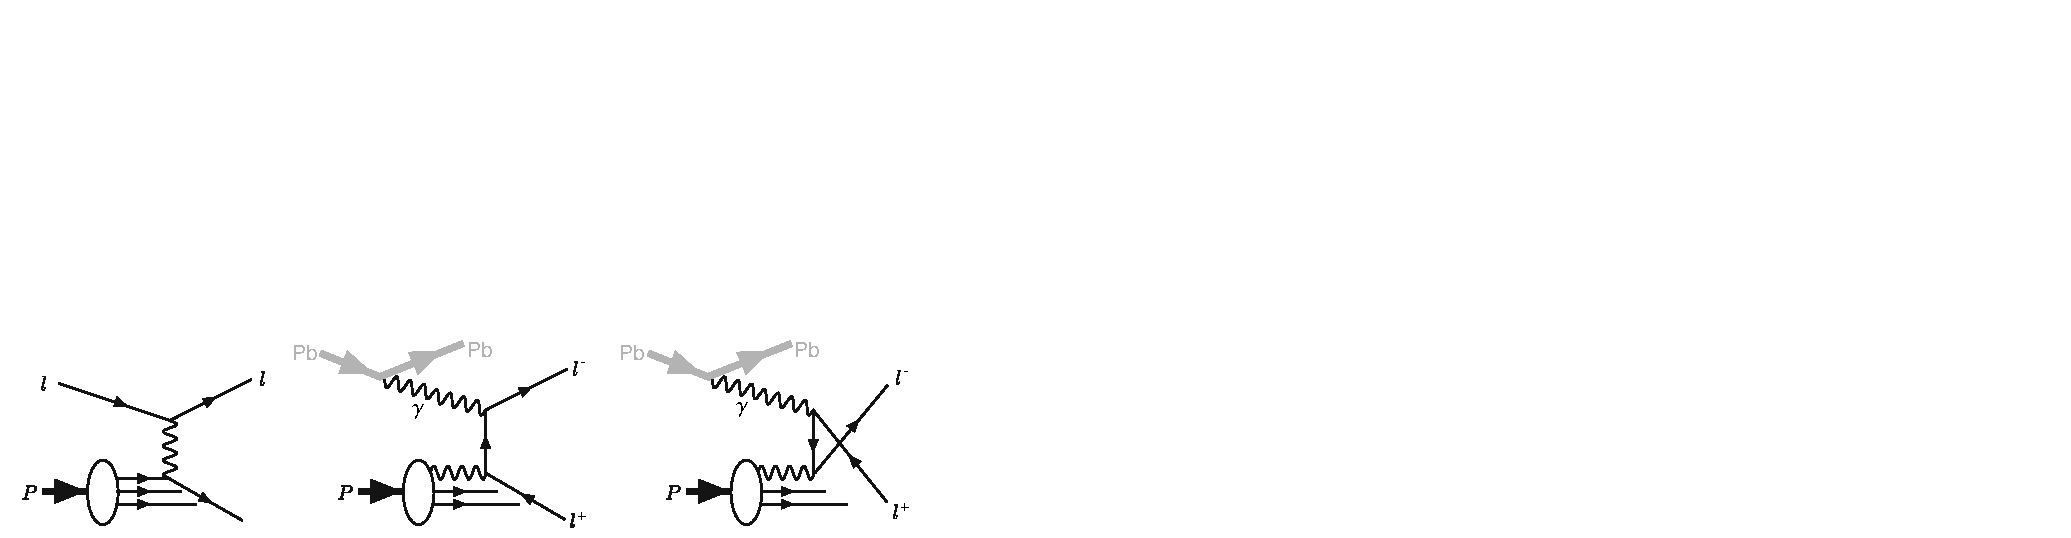
\includegraphics[width=1.\textwidth]{figures/dis_to_photon_v2.pdf}
 \put(-400,-3){{\footnotesize(a)}}
 \put(-246,-3){{\footnotesize(b)}}
\put(-90,-3){{\footnotesize(c)}}
\caption{Schematic graphs for deep inelastic scattering, $\ell^{\pm} p\rightarrow \ell^{\pm} +X$ (a) and photon-induced dilepton prodcution, $\gamma p\rightarrow \ell^+\ell^- + X$, in $p+\textrm{Pb}$ collisions for $t$-channel (b) and $u$-channel (c) lepton exchange.}
\label{fig:diagrams}
\end{figure}

Moreover, as this process does not involve the exchange of color with the photon-emitting nucleus, no significant particle production is expected in the rapidity region between the dilepton system and the nucleus. 
The photon-emitting nucleus is also expected to produce no neutrons because the photons couple to the entire nucleus. 
Thus a combination of requirements on rapidity gap and zero neutrons in the same direction provide straightforward criteria to identify these events experimentally. 




%%%%%%%%%%%%%%%%%%%%%%%%%%%%%%%%%%
\section{Formalism}
%%%%%%%%%%%%%%%%%%%%%%%%%%%%%%%%%%

%-------------------------------------
\subsection{Elastic photon fluxes}
%-------------------------------------
%In this work we are only interested in the elastic vertices on the nucleus side.

To get the distribution of the elastic photons from the proton, one can express the equivalent photon flux through
the electric and magnetic form factors $G_E(Q^2)$ and $G_M(Q^2)$ of the proton.
%%
%\begin{eqnarray}
%W^{\rm el}_T(M_X^2,Q^2) = \delta(M_X^2 - m_p^2) \, Q^2 G^2_M(Q^2) \, , \, W^{\rm el}_L(M_X^2, Q^2) = \delta(M_X^2 - m_p^2) 4m_p^2 G^2_E(Q^2) \, . 
%\end{eqnarray}
%%
This contribution is obtained as
%%
\begin{eqnarray}
  \gamma^{p}_{el}(x,Q^2) = \frac{\alpha_{\rm{em}}}{\pi}
\Big[ \Big( 1- {x \over 2} \Big)^2 \, {4 m_p^2 G_E^2(Q^2) + Q^2 G_M^2(Q^2) \over 4m_p^2 + Q^2} + {x^2 \over 4} G_M^2(Q^2) \Big]~,
\label{proton_el_flux}
\end{eqnarray}
%%
where $x$ is the momentum fraction of the proton taken by the photon, $Q^2$ is the photon virtuality, $\alpha_{\rm{em}}$ is the electromagnetic structure constant and $m_p$ is the proton mass.

To express the elastic photon flux for the nucleus, we follow Ref.~\cite{Budnev:1974de} and replace 
%%%
\begin{eqnarray}
 {4 m_p^2 G_E^2(Q^2) + Q^2 G_M^2(Q^2) \over 4m_p^2 + Q^2} \longrightarrow Z^2 F_{\rm em}^2(Q^2)~,
 \end{eqnarray}
%%%
where $F_{\rm em}(Q^2)$ is the electromagnetic formfactor of the nucleus and $Z$ is its charge.
We also neglect the magnetic formfactor of the ion in the following (it even rigorously vanishes for spinless nuclei).

For the Pb nucleus, we use the formfactor parameterization from the STARlight MC generator~\cite{Klein:2016yzr}:
%%
\begin{eqnarray}
 F_{\rm em}(Q^2) = {3 \over (QR_A)^3}\Big[ \sin(QR_A) - QR_A \cos(QR_A) \Big] { 1 \over 1 + a^2 Q^2}~,
\end{eqnarray}
%%%
where $R_A = 1.1 A^{1/3}$ fm, $a = 0.7$ fm and $Q = \sqrt{Q^2}$.
%%%

%Therefore we obtain the elastic flux
%\begin{eqnarray}
%{\cal{F}}^{{\rm{el}}}_{\gamma^* \leftarrow A} (z,\bq) = {Z^2 \alpha_{\rm{em}}\over \pi}  \, (1-z) \, 
%\Big( {\bq^2 \over \bq^2 + z (M_X^2 - m_A^2) + z^2 m_A^2  }\Big)^2 \, F^2_{\rm em}(Q^2)
%\, . \nonumber \\
%\end{eqnarray}
%%%
%For $^{208}Pb$ the charge is $Z=82$.

%----------------------------------------
\subsection{Inelastic vertices}
%----------------------------------------

We also consider the inelastic processes with breakup of a proton. 
Then the hadronic tensor is expressed in terms of the electromagnetic currents as:
%%
\begin{eqnarray}
 W^{\rm{in}}_{\mu \nu}(M_X^2,Q^2) = \overline{\sum_X} (2 \pi)^3 \, \delta^{(4)} (p_X - p_A - q) \, \bra{p} J_\mu \ket{X}\bra{X} J_\nu^\dagger \ket{p} \, d\Phi_X \, ,
\label{eq:Wmunu}
\end{eqnarray}
and its elements can be measured in inclusive electron scattering 
off the target. We wish to express it in terms of the virtual photoabsorption cross section
of transverse and longitudinal photons. To this end we introduce the covariant vectors tensors
%%
\begin{eqnarray}
e_\mu^{(0)} = \sqrt{Q^2 \over  X} \Big( p_{A\mu} - { (p_A \cdot q ) \over q^2} q_\mu \Big) \, , \, 
X = (p_A \cdot q)^2 + m_A^2 Q^2 \, , \, e^{(0)}\cdot e^{(0)} = + 1 \, ,
\end{eqnarray}
%%
and
%%
\begin{eqnarray}
\delta^\perp_{\mu \nu}(p_A,q) = g_{\mu \nu} - {q_\mu q_\nu \over q^2} - e^{(0)}_\mu e^{(0)}_\nu \, .
\end{eqnarray}
%%
Here $\delta^\perp_{\mu\nu}$ projects on photons carrying helicity $\pm 1$ in the $\gamma^* p$-cms frame,
and $e_\mu^{(0)}$ plays the role of the polarization vector of the longitudinal photon.
Notice that $q\cdot e^{0} = q^\mu \delta^\perp_{\mu \nu} = 0$, so that the hadronic tensor has the convenient
gauge invariant decomposition
%%
\begin{eqnarray}
  W^{\rm{in}}_{\mu \nu}(M_X^2,Q^2) = - \delta^\perp_{\mu \nu} (p_A,q) \, W^{\rm{in}}_T(M_X^2, Q^2) + e^{(0)}_\mu e^{(0)}_\nu \, W^{\rm{in}}_L(M_X^2, Q^2) \, .
\end{eqnarray}
The virtual photoabsorption cross sections are defined as
%%
\begin{eqnarray}
 \sigma_T(\gamma^* p) &=& {4 \pi \aem \over 4 \sqrt{X}} \, \Big(- {\delta^\perp_{\mu\nu} \over 2} \Big)  2\pi W^{\rm{in}}_{\mu \nu}(M_X^2,Q^2) \nonumber \\
 \sigma_L(\gamma^* p) &=& {4 \pi \aem \over 4 \sqrt{X}} \, e^{0}_\mu e^{0}_\nu \, 2 \pi W^{\rm{in}}_{\mu \nu}(M_X^2,Q^2) \, .
\end{eqnarray}
%%
It is customary to introduce dimensionless structure function $F_i(x_{\rm Bj},Q^2), i = T,L$ as
%%
\begin{eqnarray}
 \sigma_{T,L}(\gamma^* p) = {4 \pi^2 \aem \over Q^2} \, {1 \over \sqrt{1 + {4 x^2_{\rm Bj} m_A^2 \over Q^2}} } \, F_{T,L}(x_{\rm Bj},Q^2) \, ,
\end{eqnarray}
where
%%
\begin{eqnarray}
 x_{\rm Bj} = { Q^2 \over Q^2 + M_X^2 - m_A^2} \, .
\end{eqnarray}
%%
Then, our structure functions $W_{T,L}$ are expressed through the more conventional $F_{T,L}$ as
%%
\begin{eqnarray}
 W^{\rm{in}}_{T,L}(M_X^2,Q^2) = {1 \over x_{\rm Bj}} \, F_{T,L}(x_{\rm Bj},Q^2) \, . 
\end{eqnarray}
%%
In the literature one often finds rather $F_1(x_{\rm Bj}, Q^2), F_2(x_{\rm Bj},Q^2)$
structure functions, which are related to $F_{T,L}$ through
%%
\begin{eqnarray}
 F_T(x_{\rm Bj},Q^2) &=& 2x_{\rm Bj}  F_1(x_{\rm Bj},Q^2) \, , \nonumber \\
F_2(x_{\rm Bj},Q^2)  &=& { F_T(x_{\rm Bj},Q^2) +F_L(x_{\rm Bj},Q^2)
  \over 1 + {4 x^2_{\rm Bj} m_A^2 \over Q^2}} \; .
\end{eqnarray}
%%
Now, performing the contraction with $p^\mu_B p^\nu_B$, we get
%%
\begin{eqnarray}
  {p_B^\mu p_B^\nu \over s^2} \, W^{\rm in}_{\mu \nu}(M_X^2,Q^2) = \Big( 1 - {z \over x_{\rm Bj}} + {z^2\over 4 x_{\rm Bj}^2} \Big) {F_2(x_{\rm Bj},Q^2) \over Q^2 + M_X^2 - m_p^2} 
+ {z^2 \over 4 x^2_{\rm Bj}} { 2 x_{\rm Bj} F_1(x_{\rm Bj},Q^2) \over Q^2 + M_X^2 - m_p^2} \, .
\end{eqnarray}
%%
In the deep inelastic region $F_2 \sim F_T + F_L$, and using $2x_{\rm Bj} F_1 \sim F_2$ in the second term, we can write more succinctly
%%
\begin{eqnarray}
  {p_B^\mu p_B^\nu \over s^2} \, W^{\rm in}_{\mu \nu}(M_X^2,Q^2) = Q^2 \cdot f_T \Big( {z \over x_{\rm Bj}} \Big) \,  x_{\rm Bj} F_2(x_{\rm Bj},Q^2) \, ,
\end{eqnarray}
%%
with 
%%
\begin{eqnarray}
 f_T(y) = 1 - y + y^2/2 = {1 \over 2} \Big[ 1 + (1-y)^2 \Big] \, .
\end{eqnarray}

%-----------------------------------------------------------
\subsection{Collinear-factorization approach}
%-----------------------------------------------------------

Production of lepton pairs at large transverse momenta is a hard process, to which
standard arguments for factorization apply, and collinear factorization should be an appropriate starting point to calculate e.g. rapidity or transverse momentum spectra of leptons.
In fact, the dominant contribution to large-invariant mass dilepton pairs is of course the well known Drell-Yan process, but nothing prevents us from also including photon as partons along with quarks and gluons.

Then the photon parton distribution, $\gamma(z,Q^2)$, of photons carrying a fraction $z$ of the proton's
light-cone momentum, obeys the DGLAP equation,
%%
\begin{eqnarray}
{d \gamma(z,Q^2) \over d \log Q^2} =&& {\alpha_{\rm{em}} \over 2 \pi} \int_x^1 {dy \over y} 
\Big \{ \sum_f e_f^2 P_{\gamma \leftarrow q}(y) 
\Big[ q_f \Big({z \over y}, Q^2 \Big) + \bar q_f\Big({z \over y},Q^2\Big) \Big] \nonumber \\
&&+ P_{\gamma \leftarrow \gamma}(y) \gamma\Big({z \over y},Q^2\Big) \Big \} \, .
\end{eqnarray}
%%
In the complete set of DGLAP equations this photon density is then again coupled to the quark and antiquark
distributions:
%%
\begin{eqnarray}
 {d q_f(z,Q^2 )\over d \log Q^2} =&& {d q_f(z,Q^2) \over d \log Q^2}\Big|_{\rm{QCD}} + {\aem \over 2 \pi} \int_x^1 {dy \over y} 
\delta P_{q \leftarrow q}^{\rm{QED}}(y) q_f\Big({z \over y}, Q^2\Big)
\nonumber \\
+&& {\aem \over 2 \pi} \int_x^1 {dy \over y}  P_{q \leftarrow \gamma}(y)
\gamma\Big({z \over y},Q^2\Big) \; . \nonumber \\
\end{eqnarray}
%%
Due to the smallness of $\alpha_{\rm{em}}$ one would expect that the effect of photons on the quark and antiquark densities
can be safely neglected, unless one is interested in high order perturbative corrections to the QCD splitting functions
themselves.

Accordingly, we find two different approaches to DGLAP photons in the literature.

A first one, by Gl\"uck et al. \cite{Gluck:2002fi} asserts, that 
we can neglect the photon density on the right hand side of the evolution equations.
Then, at sufficiently large virtuality $Q_0^2$, the photon parton density can
be calculated from the collinear splitting of quarks and antiquarks 
$q \to q \gamma, \bar q \to \bar q  \gamma$. 
%%
\begin{eqnarray}
 {d \gamma(z,Q^2)\over d \log Q^2} = {\aem \over 2 \pi} \sum_f  e_f^2 \int_z^1 {dx \over x}   P_{\gamma \leftarrow q}\Big({z \over x}\Big)
\Big[ q_f(x,Q^2) + \bar q_f(x,Q^2) \Big] \; .
\label{eq:Dortmund}
\end{eqnarray}
%%
This equation is easily integrated, and gives the photon parton density as
%%
\begin{eqnarray}
 \gamma(z,Q^2) &=& \sum_f { \aem e_f^2 \over 2 \pi} \int_{Q_0^2}^{Q^2} {d \mu^2 \over \mu^2} 
\int_z^1 {dx \over x}  P_{\gamma \leftarrow q}\Big({z \over x}\Big)
\Big[ q_f(x,\mu^2) + \bar q_f(x,\mu^2) \Big] + \gamma(z,Q_0^2) \nonumber \\
&=& {\aem \over 2 \pi} \int_{Q_0^2}^{Q^2} {d \mu^2 \over \mu^2} \int_z^1 {dx \over x}  
P_{\gamma \leftarrow q}\Big({z \over x}\Big) {F_2(x,\mu^2) \over x} 
+ \gamma(z,Q_0^2) \, .
\end{eqnarray}
%%
One is left to specify -- from some  model considerations -- the photon density at some low scale $\gamma(z,Q_0^2)$, but
one may hope that at very large $Q^2 \gg Q_0^2 \sim 1 \, {\rm GeV}^2$ the part predicted perturbatively 
from quark and antiquark distributions dominates.

In addition to the above contribution from DGLAP splitting, Gl\"uck et
al. also add the Weizs\"acker-Williams flux from the coherent emission 
$p \to p \gamma^*$ without proton breakup as found in \cite{Budnev:1974de}.
 
The Durham \cite{Martin:2004dh,Martin:2014nqa} and NNPDF 
\cite{Ball:2013hta} groups have given a more involved treatment, 
in which the photon distribution is fully incorporated into the coupled 
DGLAP evolution equation.
As usual with DGLAP evolution, the photon parton density at a starting scale 
$\gamma(z,Q_0^2)$ needs to be specified. While \cite{Martin:2004dh,Martin:2014nqa} present model approaches, in Ref.\cite{Ball:2013hta} an ambitious attempt to
obtain $\gamma(z,Q_0^2)$ from a fit to experimental data is found.
Preliminary work by the CTEQ collaboration \cite{Schmidt:2014aba} is
also based on QED corrected DGLAP equations,
and attempts to fit the photon distribution from the prompt photon
production $e p \to \gamma e X$ at HERA
where in part of the phase space the Compton subprocess $e \gamma \to e \gamma$ contributes.

It should be noted, that in the approach of
\cite{Martin:2004dh,Martin:2014nqa}, the input distribution $\gamma(z,Q_0^2)$ contains the coherent --or elastic-- contribution with an intact proton in the final state.
Notice that due to the proton form factors the integral over
virtualities in the elastic case quickly converges, and the elastic
contribution is basically independent of $Q_0^2$, as soon as $Q_0^2 \gsim 0.7 \, \rm{GeV}^2$.


In the collinear approach the photon-photon contribution
to inclusive cross section for dilepton production can be written as:
%
\begin{equation}
{d \sigma^{(i,j)} \over d y_1 d y_2 d^2 p_T} 
= {1 \over 16 \pi^2 (x_1 x_2 s)^2}\sum_{i,j} 
x_1 \gamma^{(i)}(x_1,\mu^2) 
x_2 \gamma^{(j)}(x_2,\mu^2)
\overline{ |{\cal M}_{\gamma \gamma \rightarrow l^+ l^-}|^2 }.
\label{collinear_factorization_formula}
\end{equation}
%
Here 
%
\begin{eqnarray}
 x_1 &=&  \sqrt{p_T^2 + m_l^2 \over s} 
\Big( \exp(y_1) + \exp(y_2) \Big) \; , \nonumber \\
 x_2 &=&  \sqrt{p_T^2 + m_l^2 \over s} 
\Big( \exp(-y_1) + \exp(-y_2) \Big) \; . 
\end{eqnarray}
%%
Above indices $i$ and $j$ denote $i,j = \rm{el, in}$, i.e. they
correspond to elastic or inelastic components similarly as for 
the $k_T$-factorization discussed in section below.
The factorization scale is chosen as $\mu^2 = m_T^2 = p_T^2 + m_l^2$ (Renat?)

%%%%%%%%%%%%%%%%%%%%%%%%%%%%%%%%%%
\section{Example experimental configuration and possible background sources}
%%%%%%%%%%%%%%%%%%%%%%%%%%%%%%%%%%
\label{sec:experiment}

We assume collision setup from recent $p+\textrm{Pb}$ run at the LHC, carried out at the centre-of-mass energy per nucleon pair $\sqrt{s_{N N}} = 8.16$~\TeV.
Since the energy per nucleon in the proton beam is larger than in the lead beam, the nucleon--nucleon centre-of-mass system has a rapidity in the laboratory frame of $y = 0.465$.

As an example of method's applicability, we will use the geometry of ATLAS~\cite{Aad:2008zzm} and CMS~\cite{Chatrchyan:2008aa} detectors in the following.
We consider only the dimuon channel, however the integrated results for $ee$ and $\mu\mu$ channels can be obtained by simply multiplying the dimuon cross-sections by a factor of two.


We start by applying a minimum transverse momentum requirement of 4~\GeV\ to both muons.
This requirement is imposed to ensure high lepton reconstruction and triggering efficiency.
% in the ATLAS and CMS experiments during LHC's $p+\textrm{Pb}$ runs~\cite{}.
Moreover, due to limited acceptance of the detectors, each muon is required to have a pseudorapidity ($\eta^{\ell}$) that satisfies $|\eta^{\ell}|<2.4$.
Our calculations are carried out for a minimum dilepton invariant mass of $m_{\ell^+\ell^-} = 10$~\GeV. 
Such a choice is due to removal of possible contamination from $\Upsilon(\rightarrow \ell^+\ell^-)$ photoproduction.
A summary of all selection requirements is presented in Table~\ref{tab:fidRegion}.

\begin{table}[t!]
  \begin{center}
    \begin{tabular}{|l|c|}
      \hline 
    Variable  & Requirement \\ \hline
    lepton transverse momentum, $p_{\textrm{T}}^{\ell}$ & $>4$~\GeV \\
    lepton pseudorapidity, $|\eta^\ell|$ & $<2.4$ \\
    dilepton invariant mass, $m_{\ell^+\ell^-}$ & $>10$~\GeV  \\
      \hline 
    \end{tabular}
  \end{center}
  \caption{Definition of the fiducial region used in the studies.}
  \label{tab:fidRegion}
\end{table}

% thinking of moving this part in the intruduction...
%As the signal process does not involve the exchange of color with the photon-emitting nucleus, no significant particle production is expected in the rapidity region between the dilepton system and the nucleus. 
%The photon-emitting nucleus is also expected to produce no neutrons because the photons couple to the entire nucleus. 
%Thus a combination of a rapidity gap and zero neutrons in the same direction provide straightforward criteria to identify these events experimentally. 

Possible background for this process can arise from inclusive lepton-pair production, e.g. from Drell--Yan process~\cite{Drell:1970wh,Aad:2015gta,Khachatryan:2015pzs,Alice:2016wka}.
This processes would lead to disintegration of the incoming ion, and zero-degree calorimeters (ZDC)~\cite{Dellacasa:1999ke,ATLAS:2007aa} can be used to veto very-forward-going neutral fragments which would allow this background 
to be reduced fully.
Another background can arise from diffractive interactions, hence possibly mimicking the signal topology.
However, since the Pb nucleus is a fragile object (with the nucleon binding energy of just 8 MeV) even the softest diffractive interaction will likely result in the emission of a few nucleons from the ion, detectable in the ZDC.

Another background category is the photon-induced process with a resolved photon, i.e. 
$\gamma p\rightarrow Z/\gamma^*+X$ reaction.
Here, the rapidity gap is expected to be smaller than in the signal process due to the additional particle production associated with the ``photon remnant''.
Any other residual contamination of this process can be controlled using a dedicated sample, with a dilepton invariant mass around the $Z$-boson mass.




%%%%%%%%%%%%%%%%%%%%%%%%%%%%%%%%%%
\section{Results with collinear photon-PDFs}
%%%%%%%%%%%%%%%%%%%%%%%%%%%%%%%%%%

We start with the calculation of the elastic contribution, $p+\textrm{Pb}\rightarrow p+\textrm{Pb}+ \ell^+\ell^-$.
In this case the photon flux becomes:
\begin{equation}
f_\gamma^{p}(x,\mu) = f_\gamma^{p}(x) 
\end{equation}
and the following parameterization is used~\cite{}:
\begin{equation}
f_\gamma^{p}(x) = \frac{\alpha}{\pi}
\left(
\frac{1-x+0.5x^2}{x}
\right)
\left(
\frac{A+3}{A-1}\log{A}-\frac{17}{6}-\frac{4}{3A}+\frac{1}{6A^2}
\right)~,
\end{equation}
where $A = 1+\frac{Q_0^2(1-x)}{x m_p^2}$ and $Q_0^2 = 0.71$~\GeV$^2$.

The results for the elastic case are cross-checked with the calculation from STARlight MC and a good agreement is found:
$\sigma_{fid}^{\textrm{el}} = 17.5$~nb, whereas $\sigma_{fid}^{\textrm{STARlight}} = 17.0$~nb.
Both calculations are also corrected by a factor $S^2=0.96$ which takes into account the requirement that there be no hadronic interactions between the proton and the ion. This is calculated using STARlight, where the hard-sphere proton--nucleus requirement~\cite{Klein:2016yzr} is used.

Next, for the inelastic case ($\gamma p\rightarrow \ell^+\ell^- + X$), several recent parameterizations of the photon parton distributions are studied: CT14qed~\cite{Schmidt:2015zda}, LUXqed17~\cite{Manohar:2017eqh} and NNPDF3.1luxQED~\cite{Bertone:2017bme}.
Comparison of several lepton kinematic distributions between different photon-PDFs are shown in Fig.~\ref{fig:elastic},\ref{fig:elastic_cut},\ref{fig:inc},\ref{fig:inc_cut}.

\begin{figure}[h!]
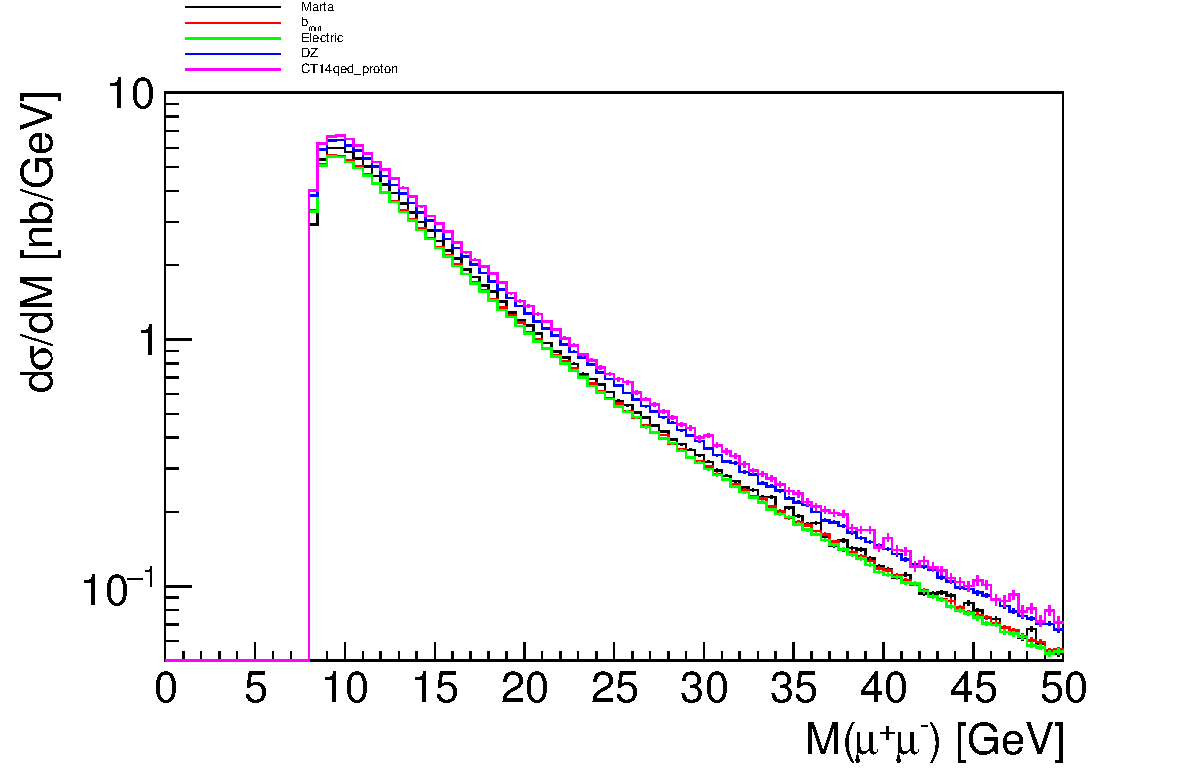
\includegraphics[width=0.4\textwidth]{figures/Mll_elastic.pdf}
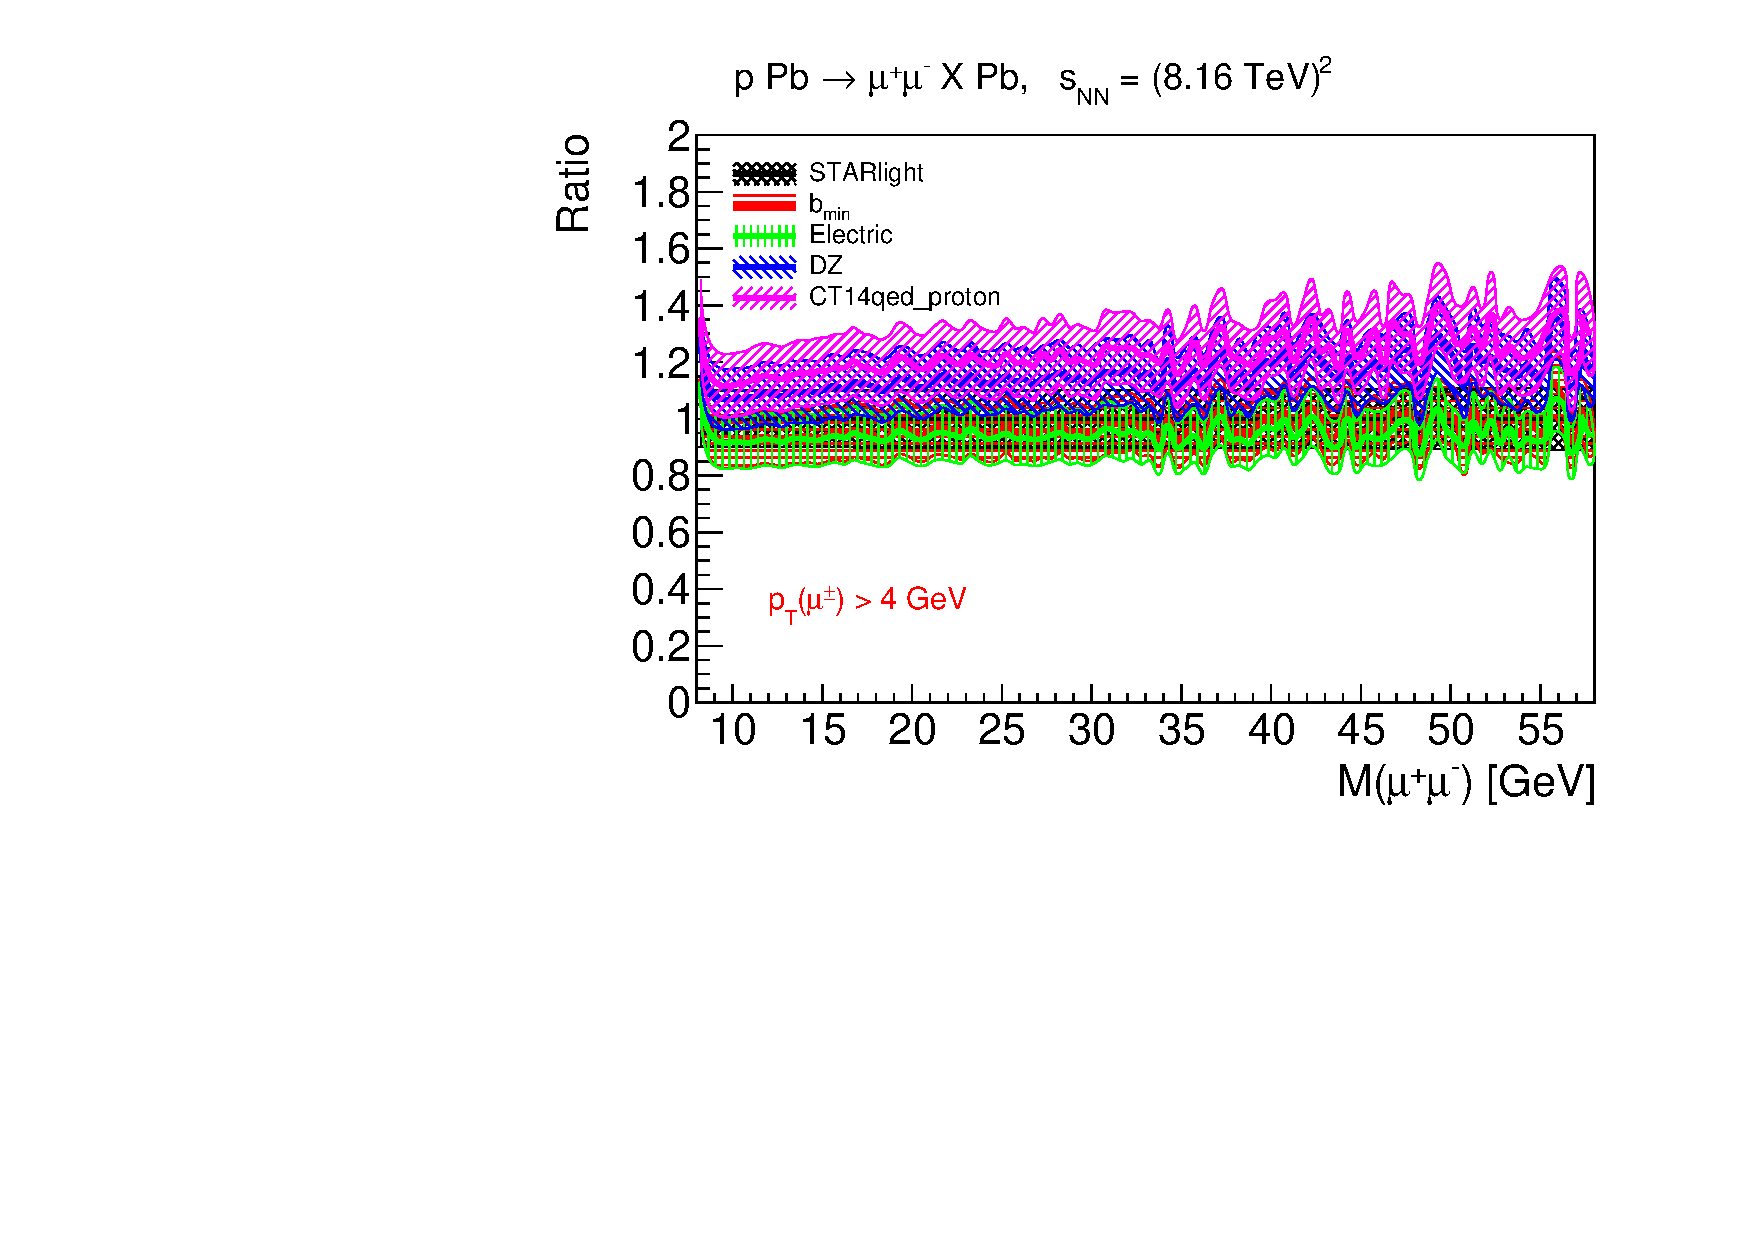
\includegraphics[width=0.4\textwidth]{figures/RatioMll_elastic.pdf}
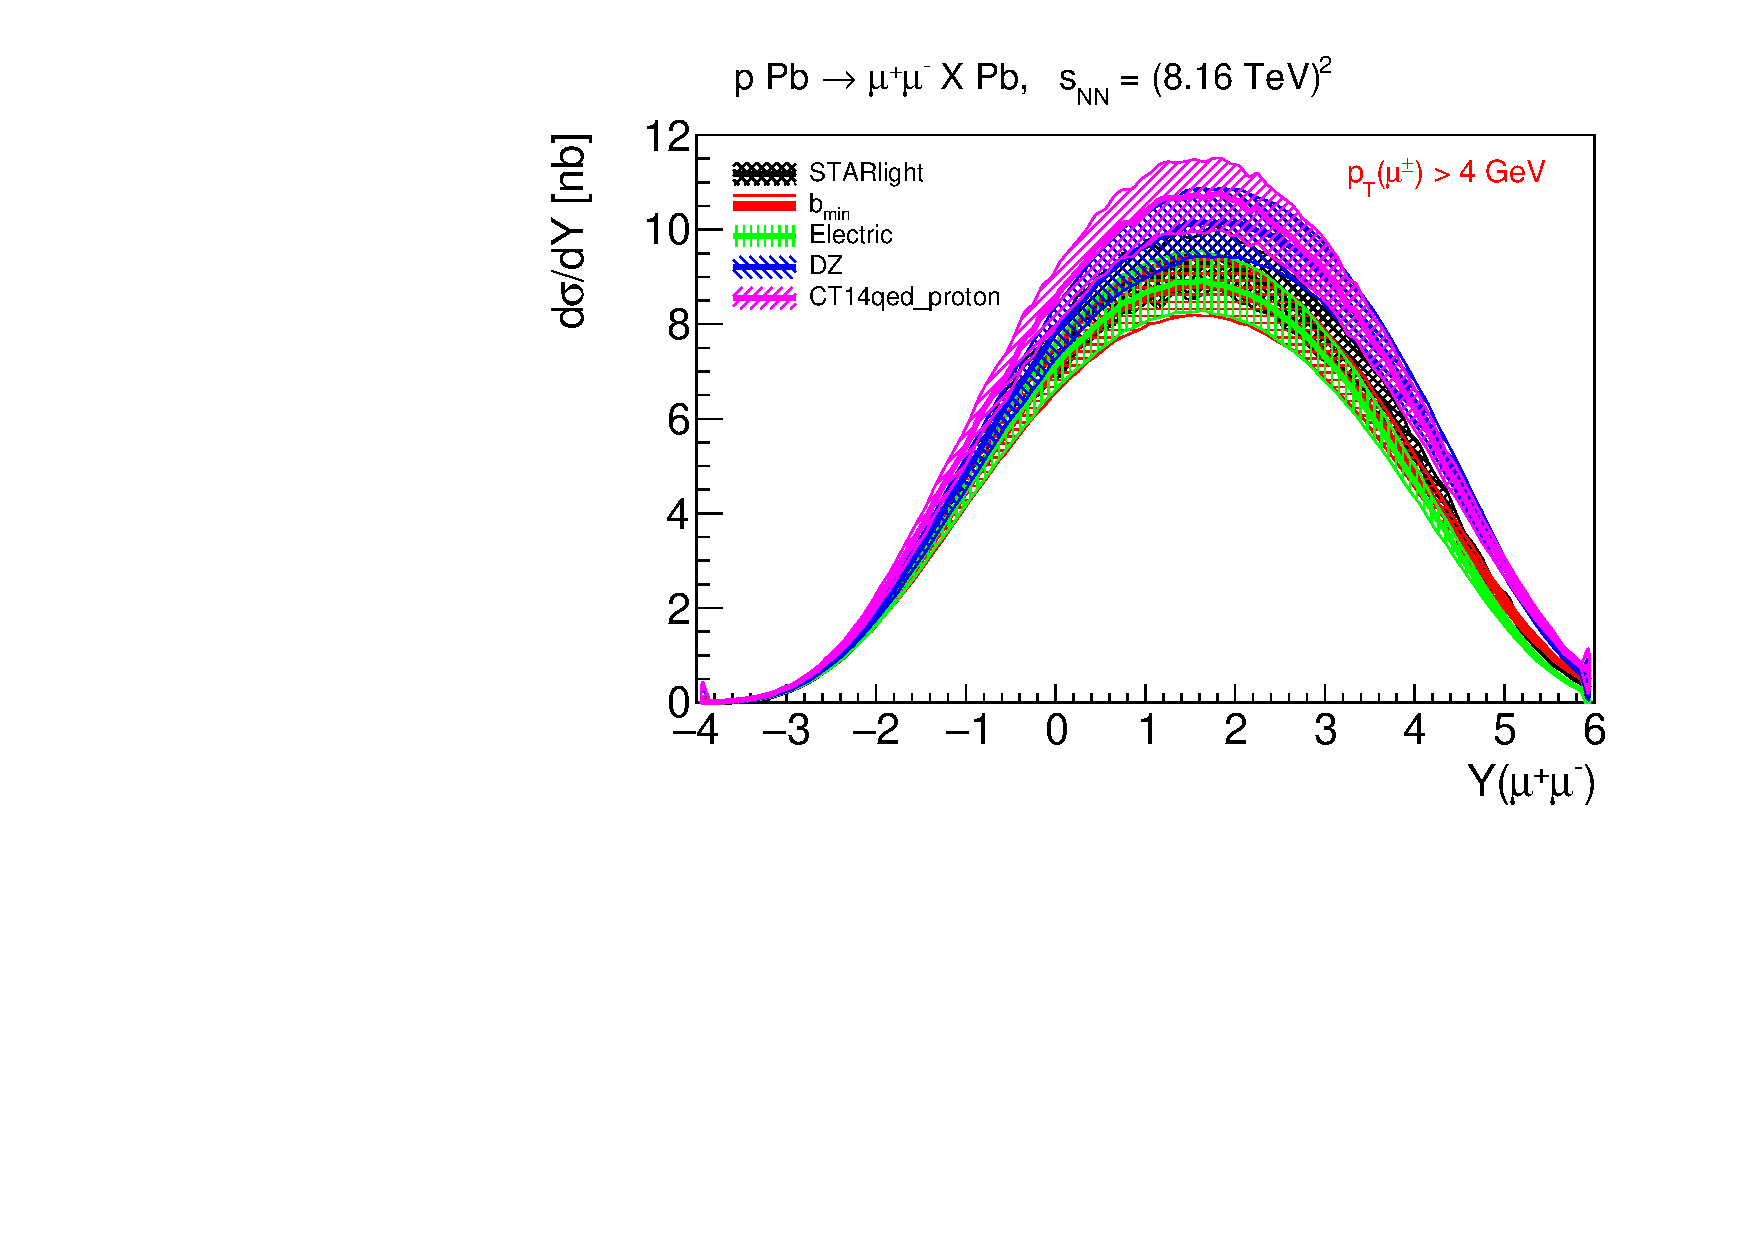
\includegraphics[width=0.4\textwidth]{figures/Yll_elastic.pdf}
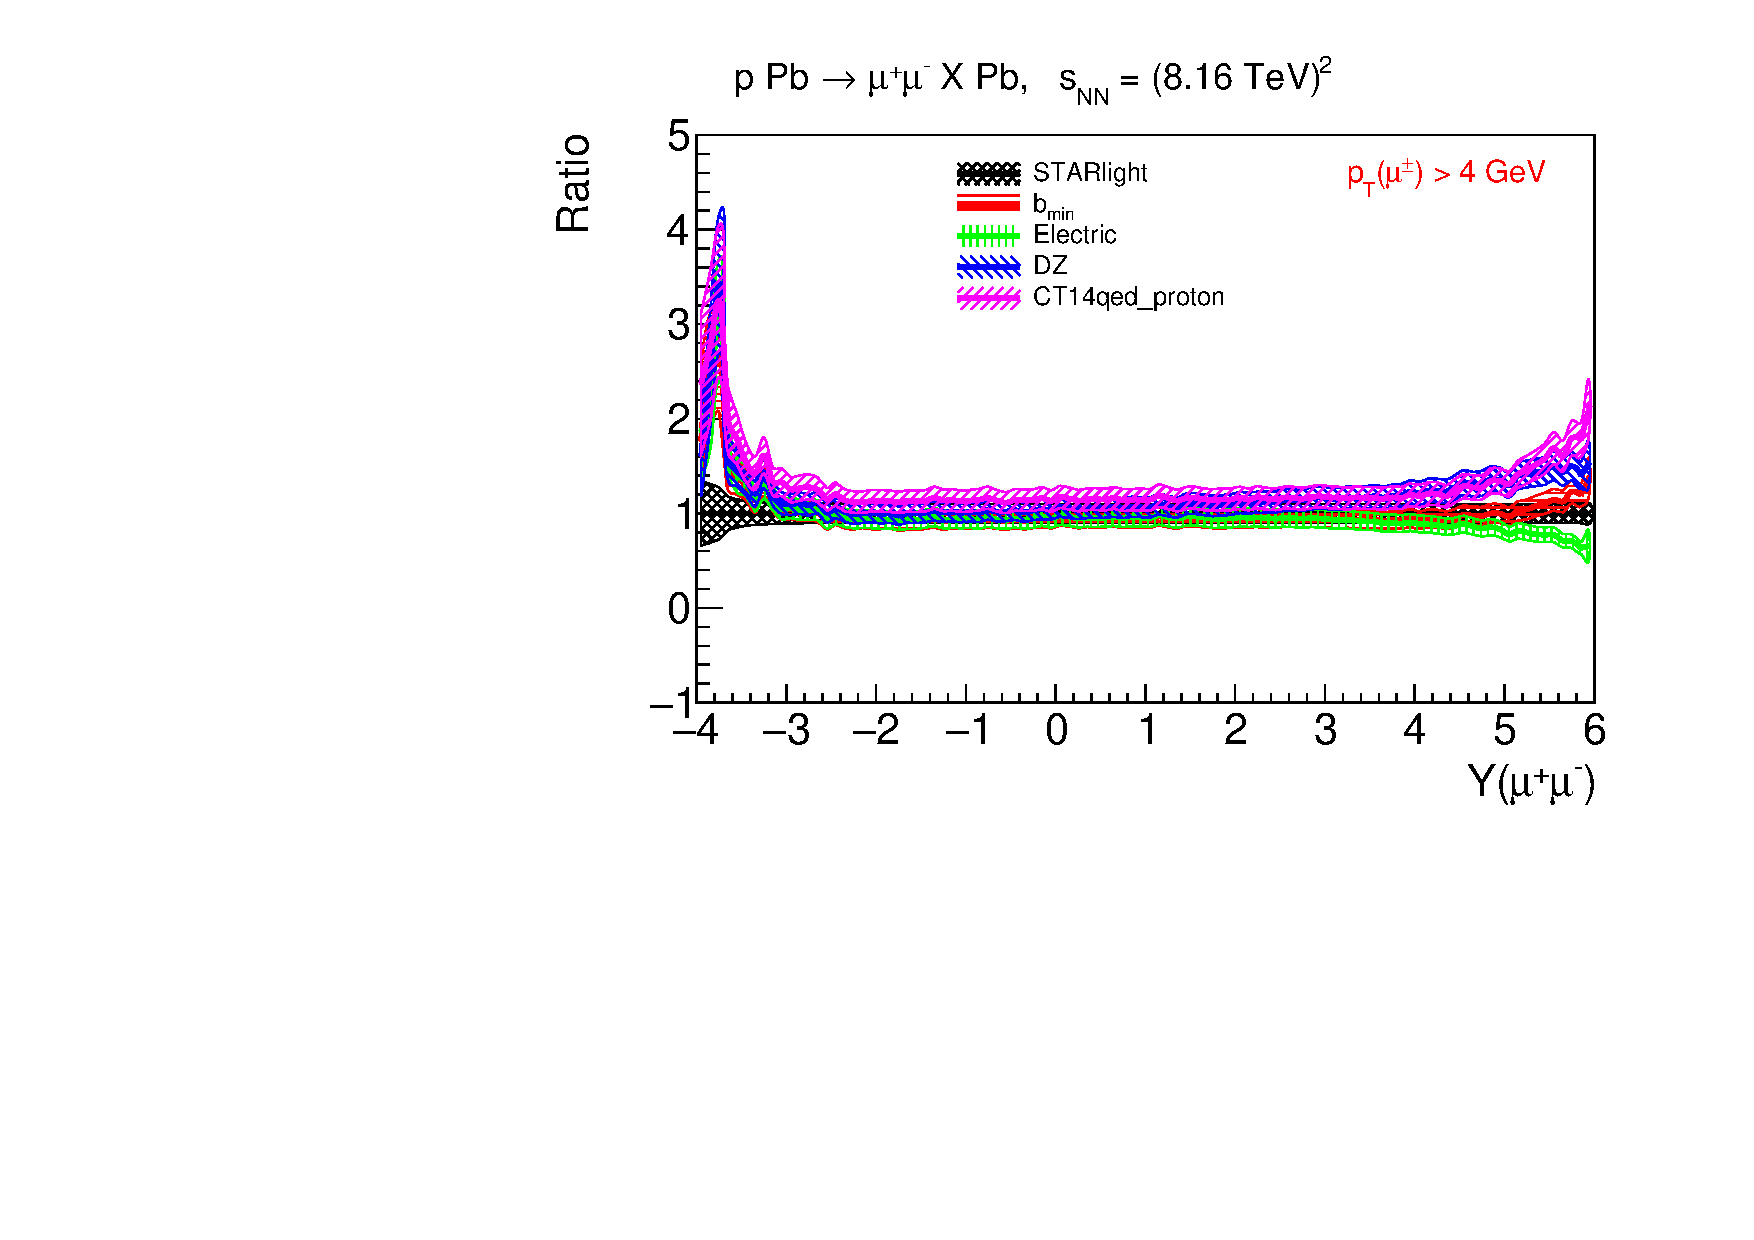
\includegraphics[width=0.4\textwidth]{figures/RatioYll_elastic.pdf}
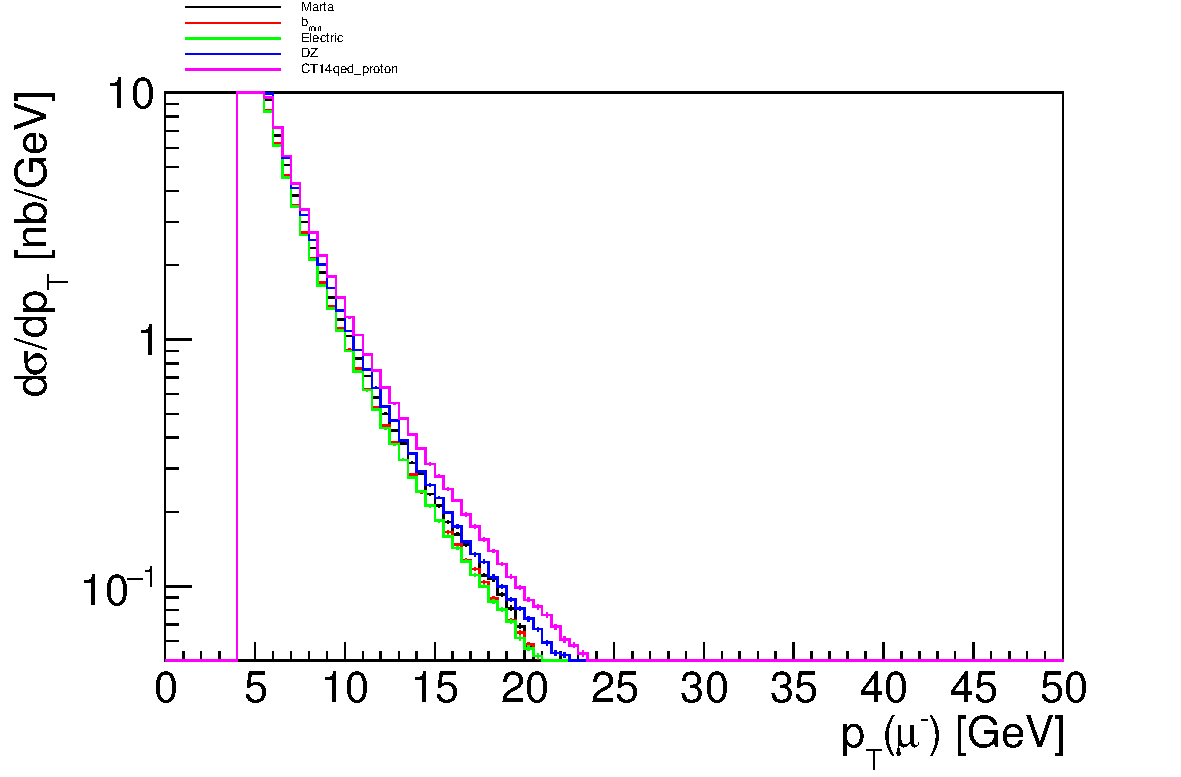
\includegraphics[width=0.4\textwidth]{figures/pTl_elastic.pdf}
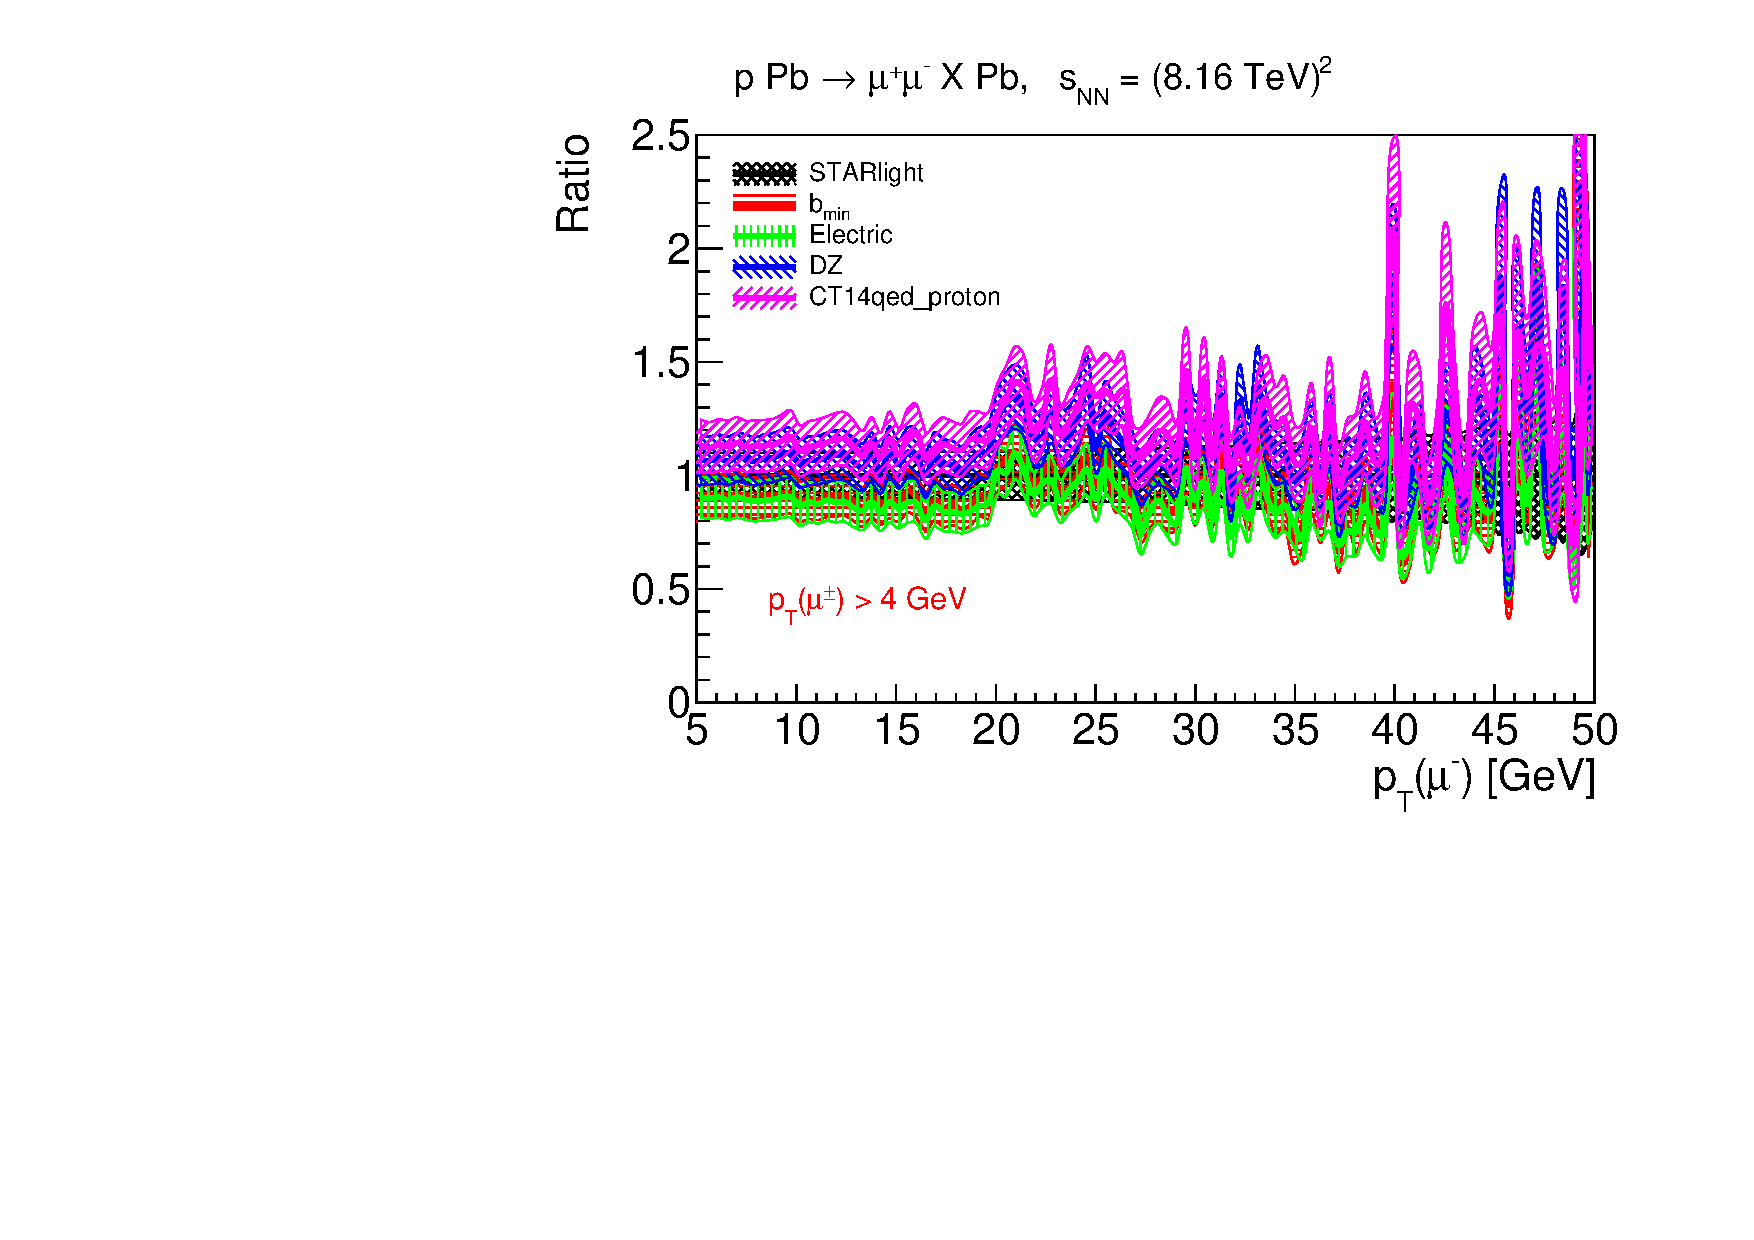
\includegraphics[width=0.4\textwidth]{figures/RatiopTl_elastic.pdf}
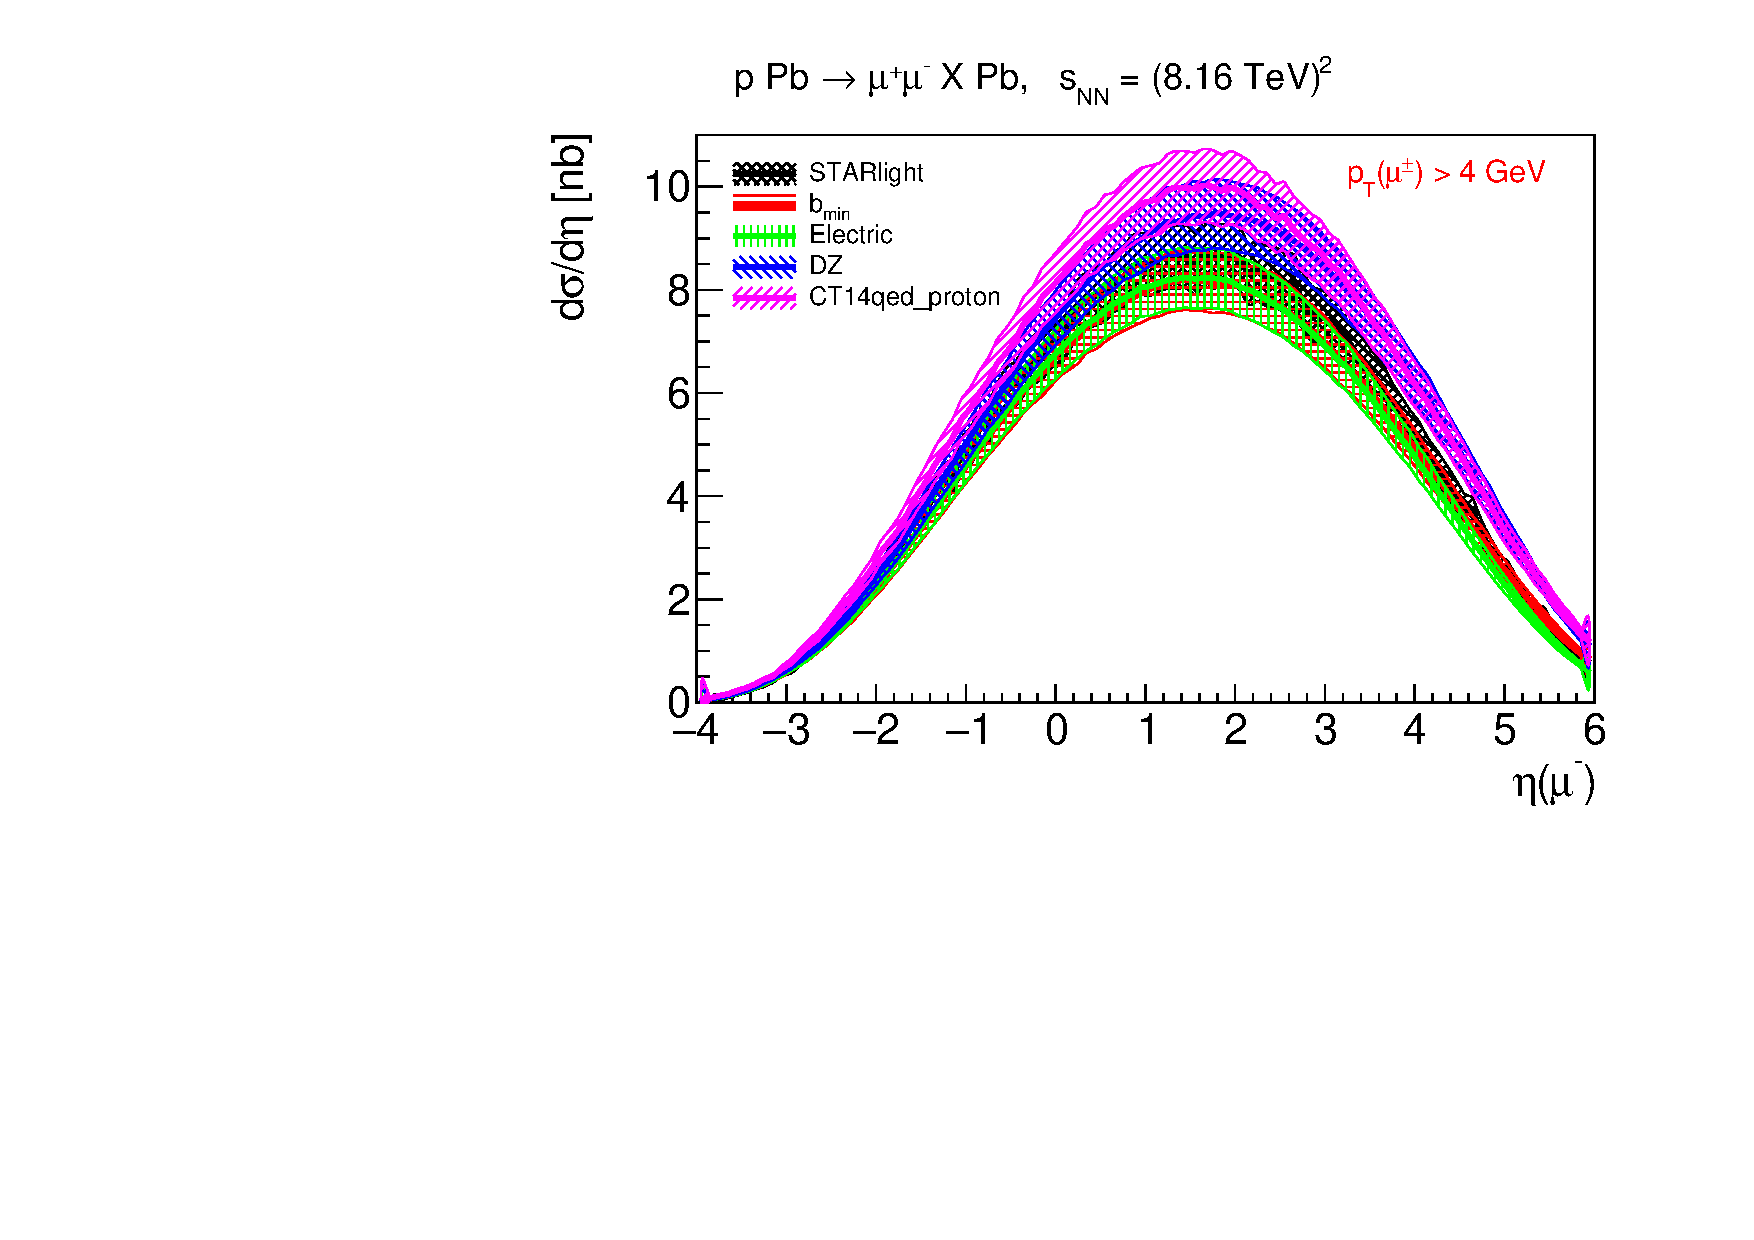
\includegraphics[width=0.4\textwidth]{figures/etal_elastic.pdf}
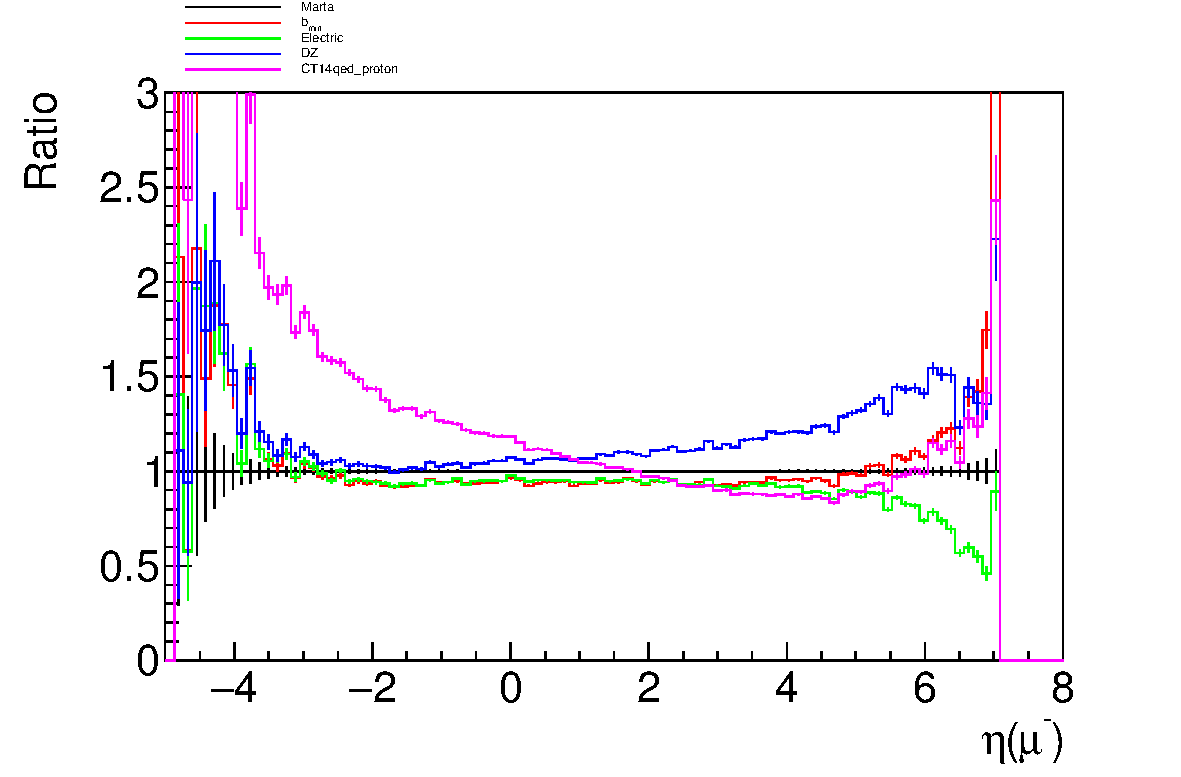
\includegraphics[width=0.4\textwidth]{figures/Ratioetal_elastic.pdf}
\caption{Elastic distributions (the only cut is on leptons $p_T$)}
\label{fig:elastic}
\end{figure}

\begin{figure}[h!]
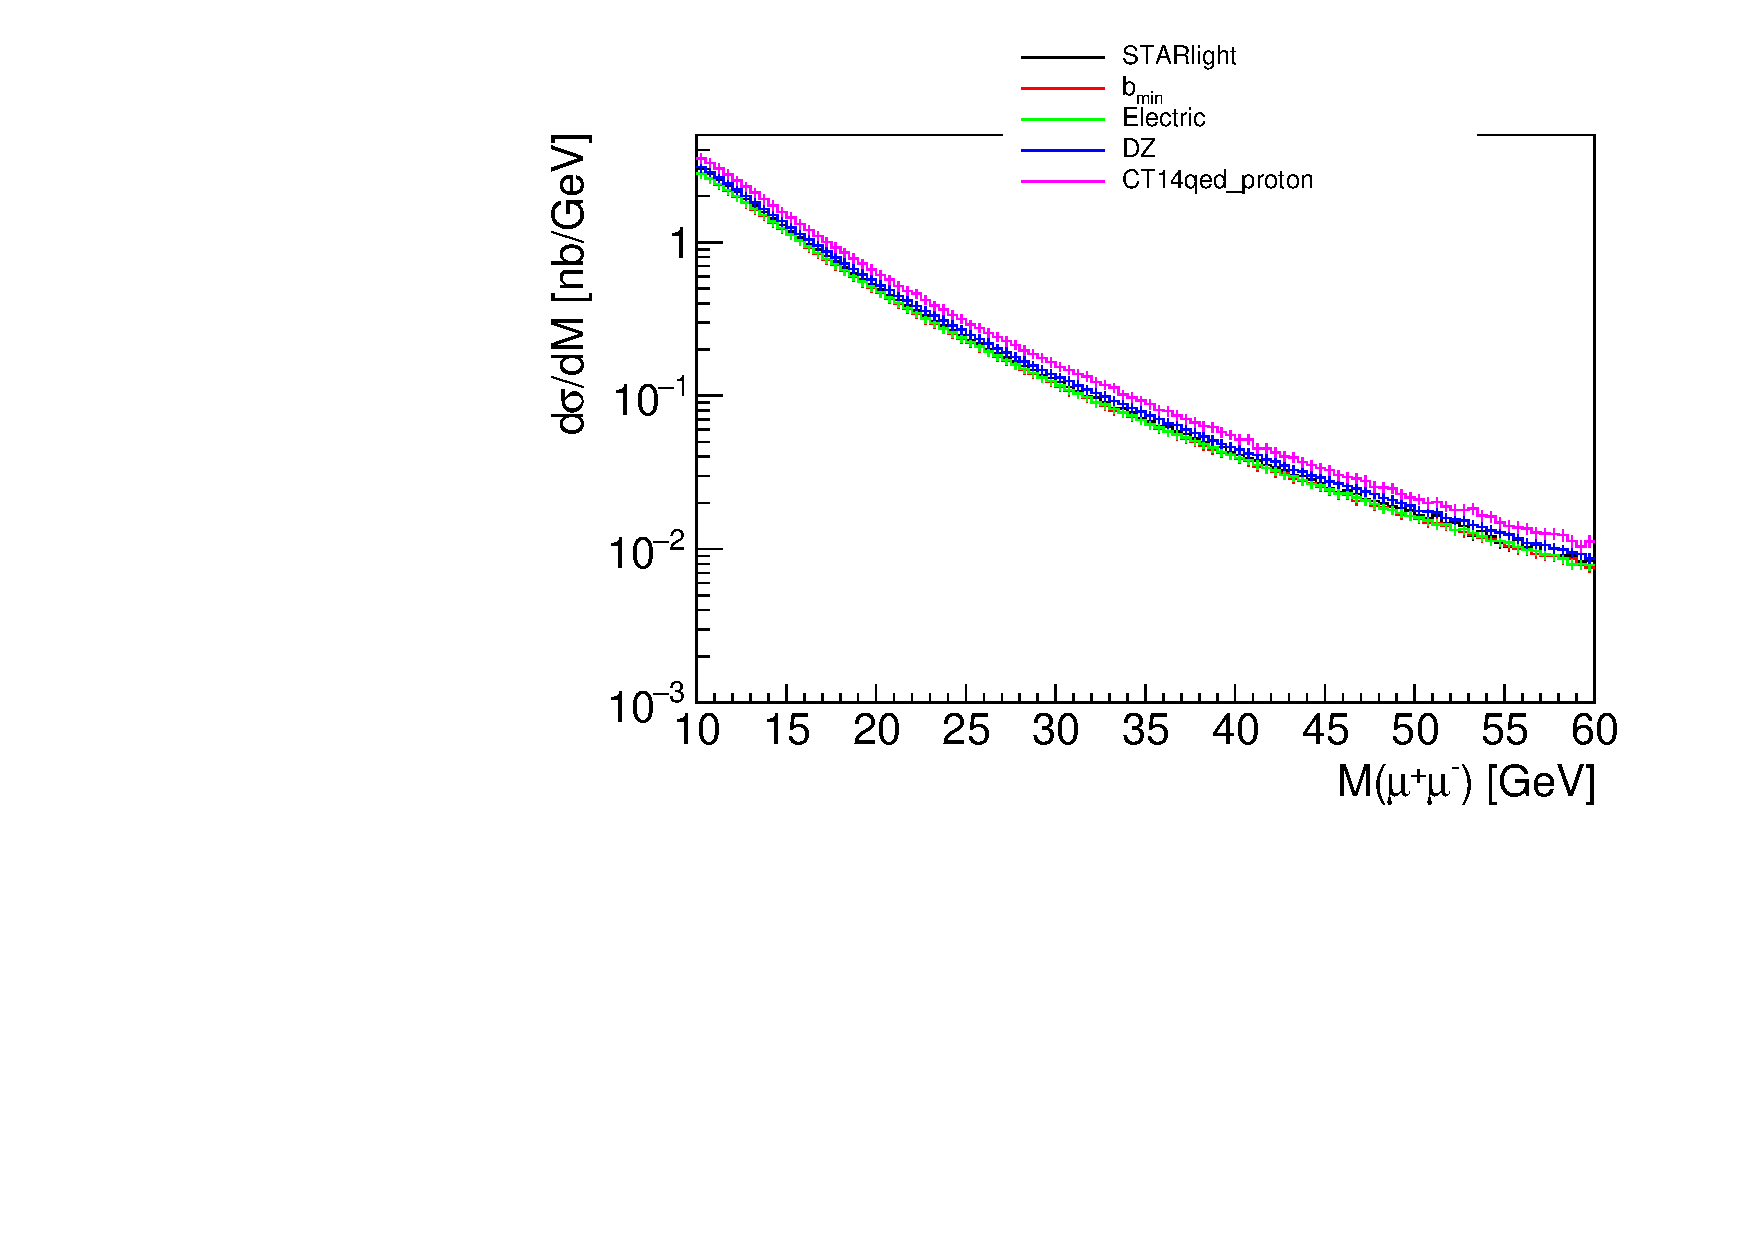
\includegraphics[width=0.4\textwidth]{figures/Mll_elastic_cut.pdf}
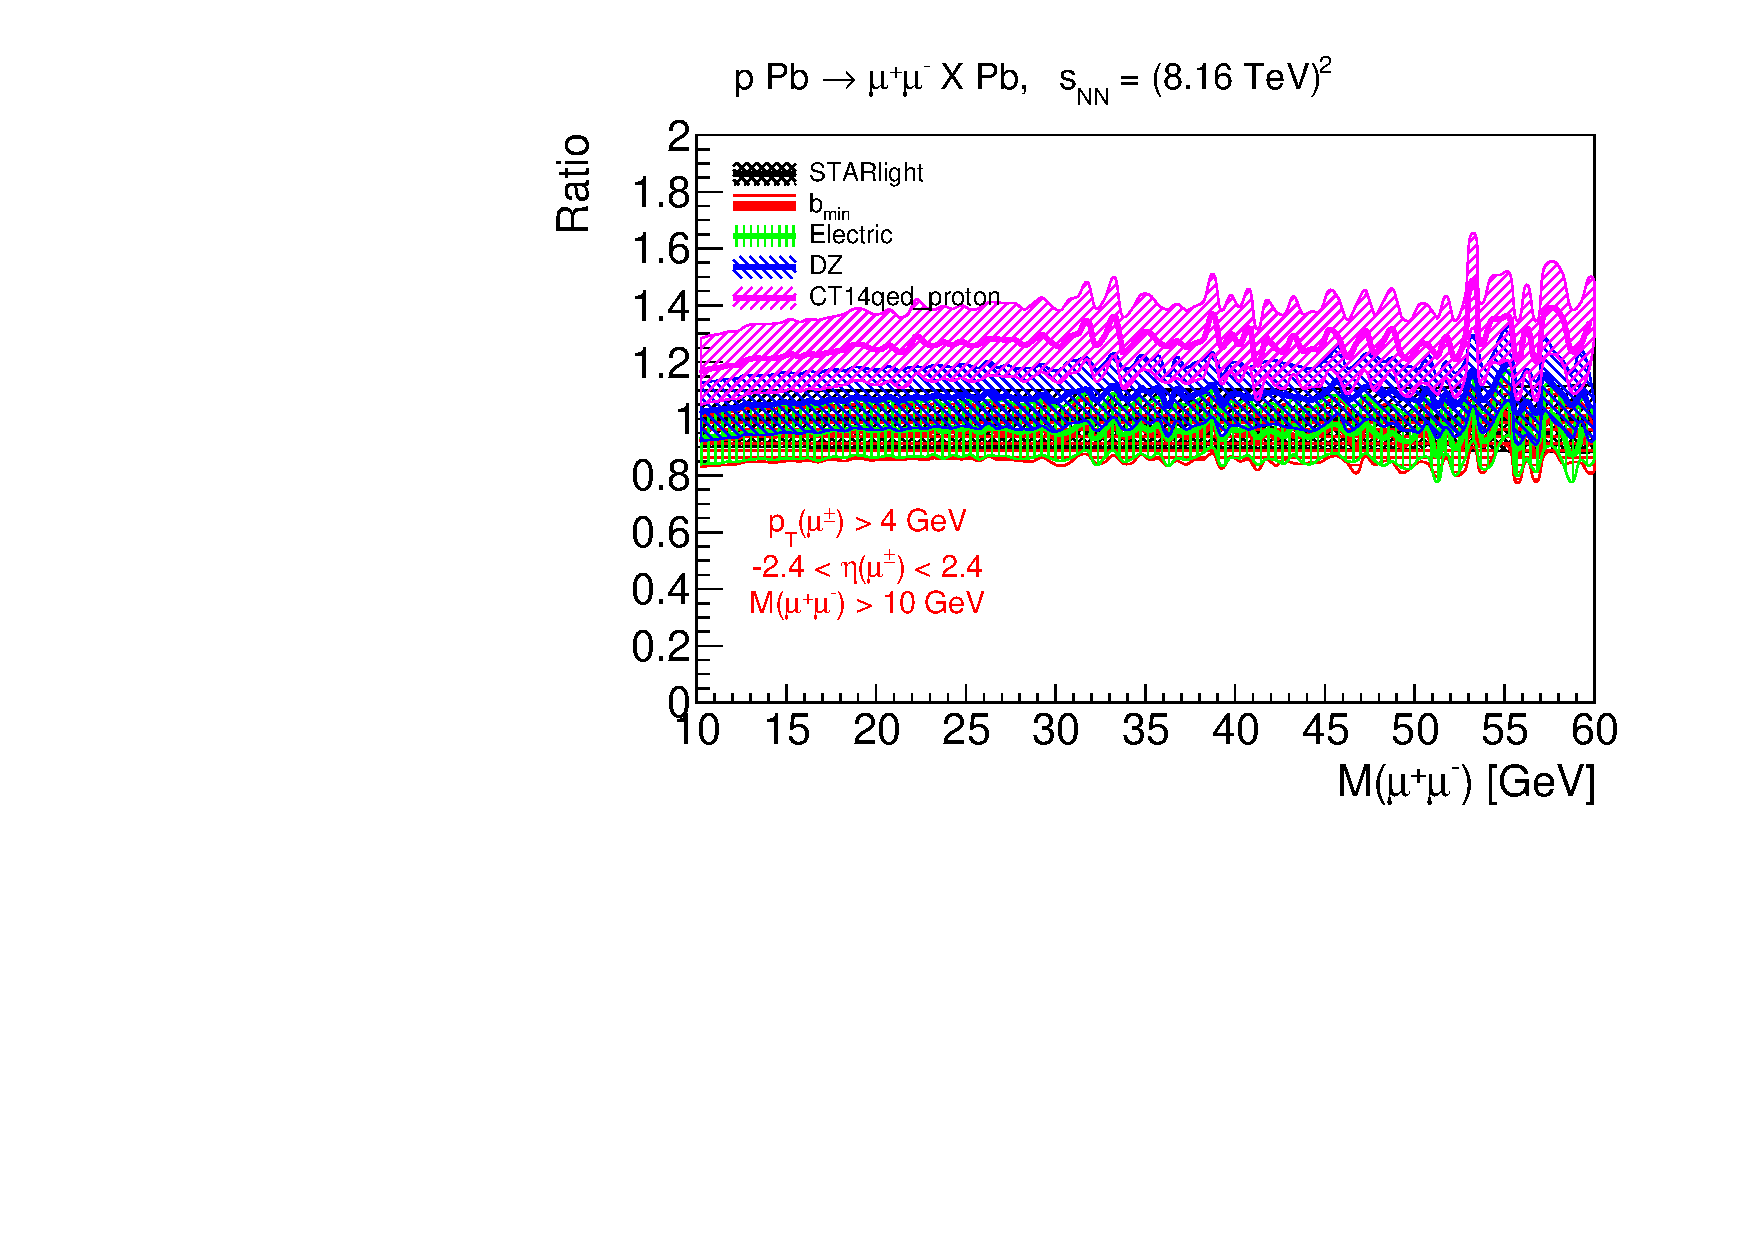
\includegraphics[width=0.4\textwidth]{figures/RatioMll_elastic_cut.pdf}
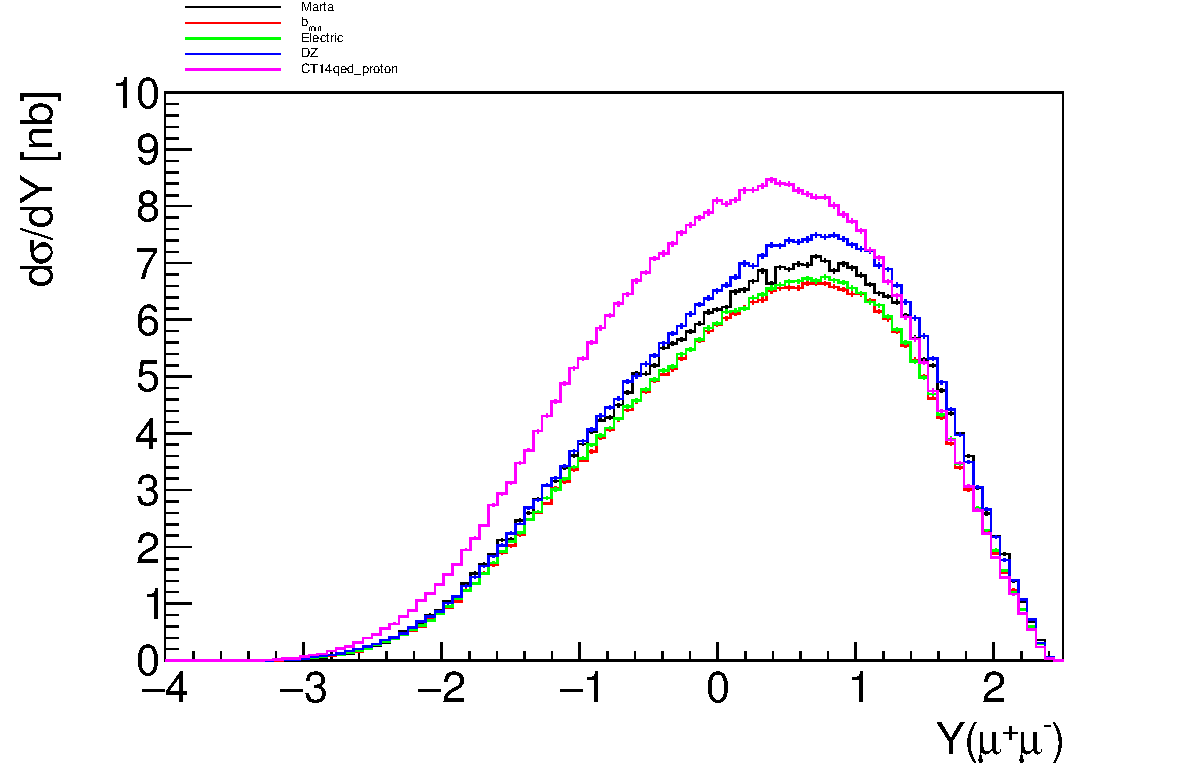
\includegraphics[width=0.4\textwidth]{figures/Yll_elastic_cut.pdf}
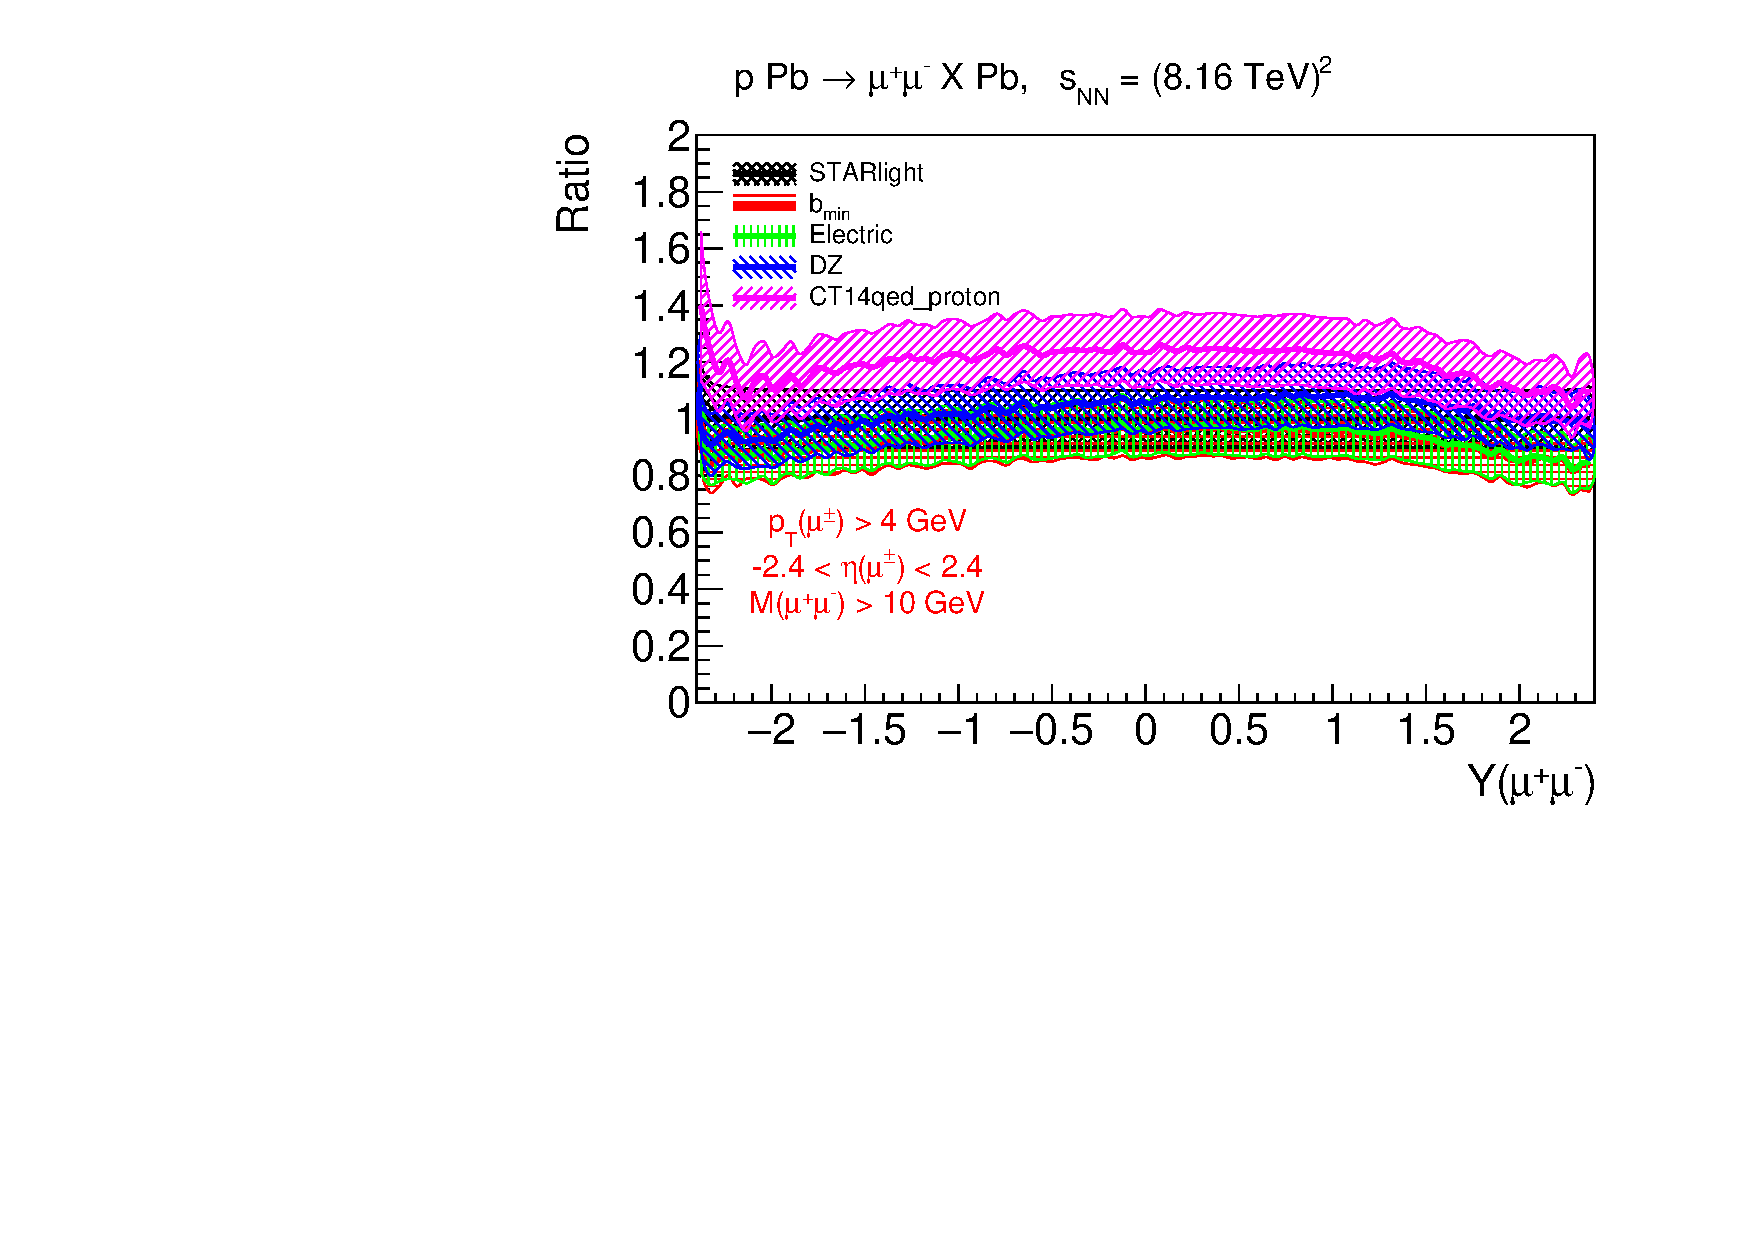
\includegraphics[width=0.4\textwidth]{figures/RatioYll_elastic_cut.pdf}
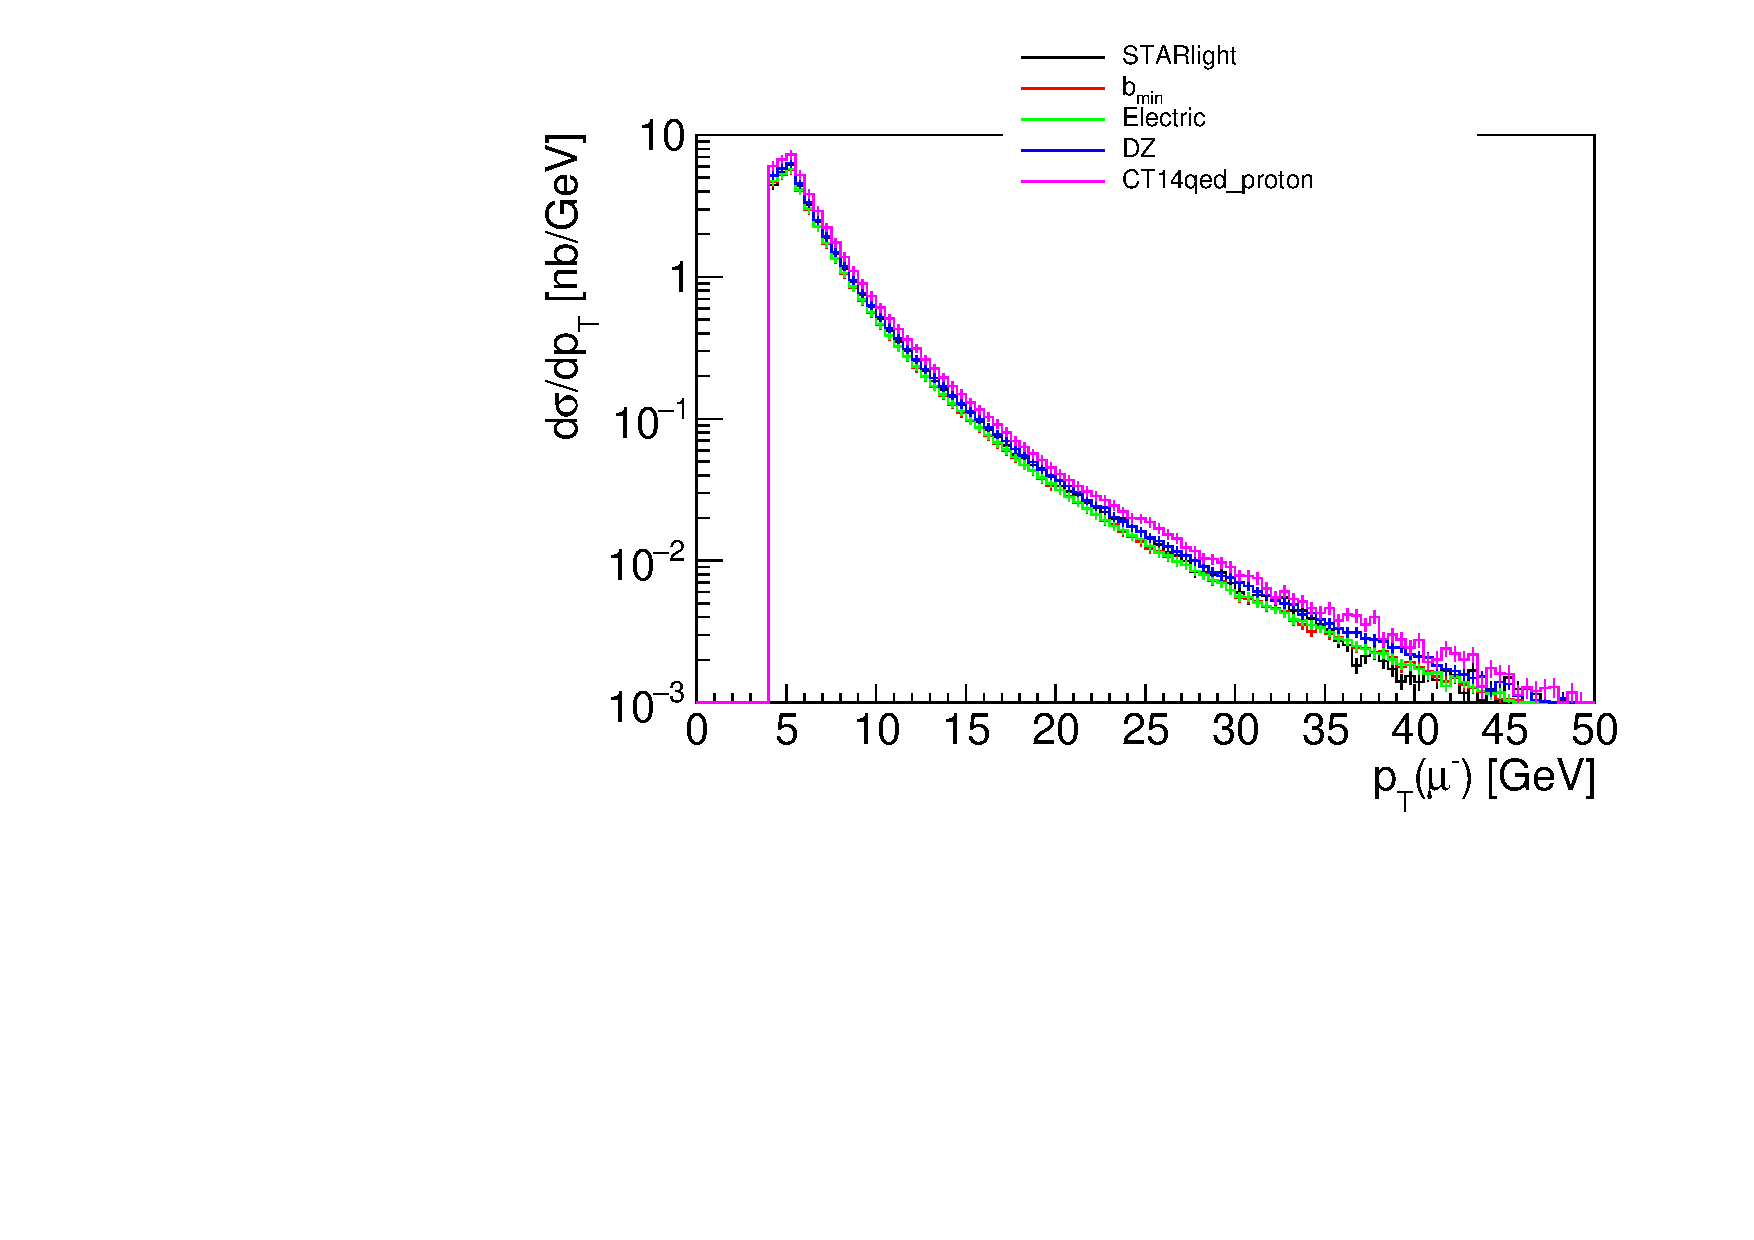
\includegraphics[width=0.4\textwidth]{figures/pTl_elastic_cut.pdf}
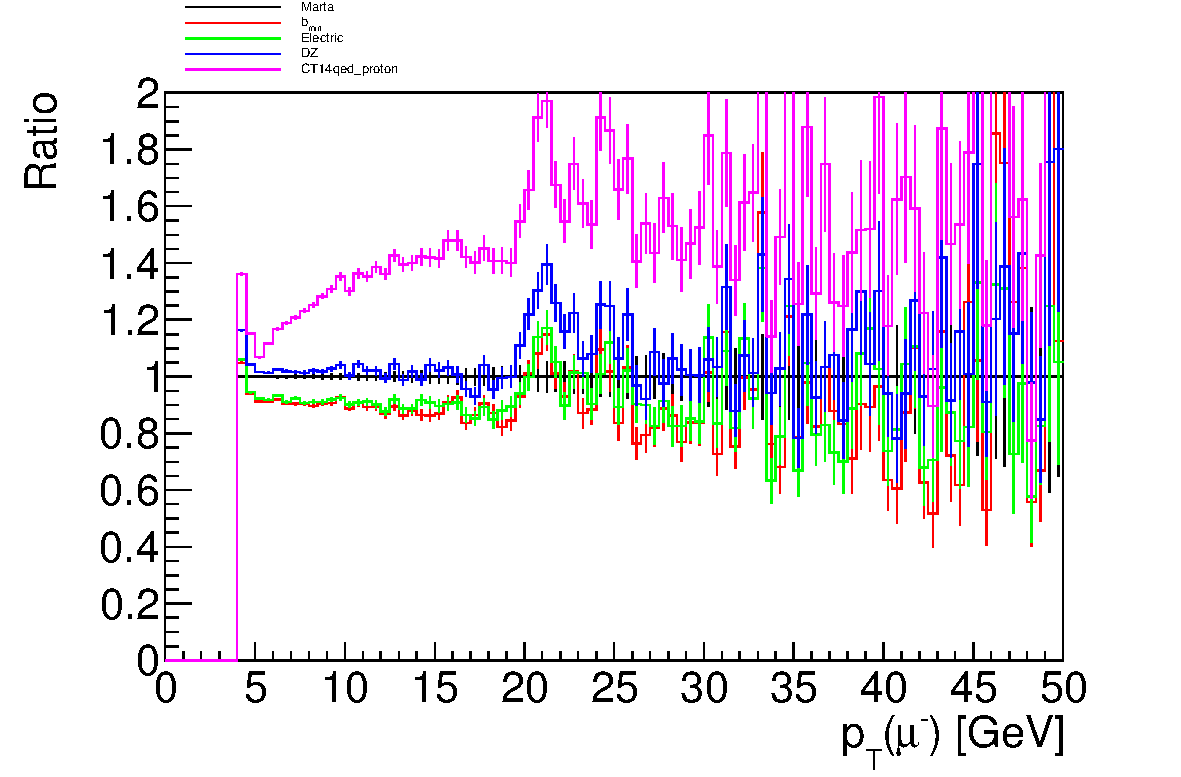
\includegraphics[width=0.4\textwidth]{figures/RatiopTl_elastic_cut.pdf}
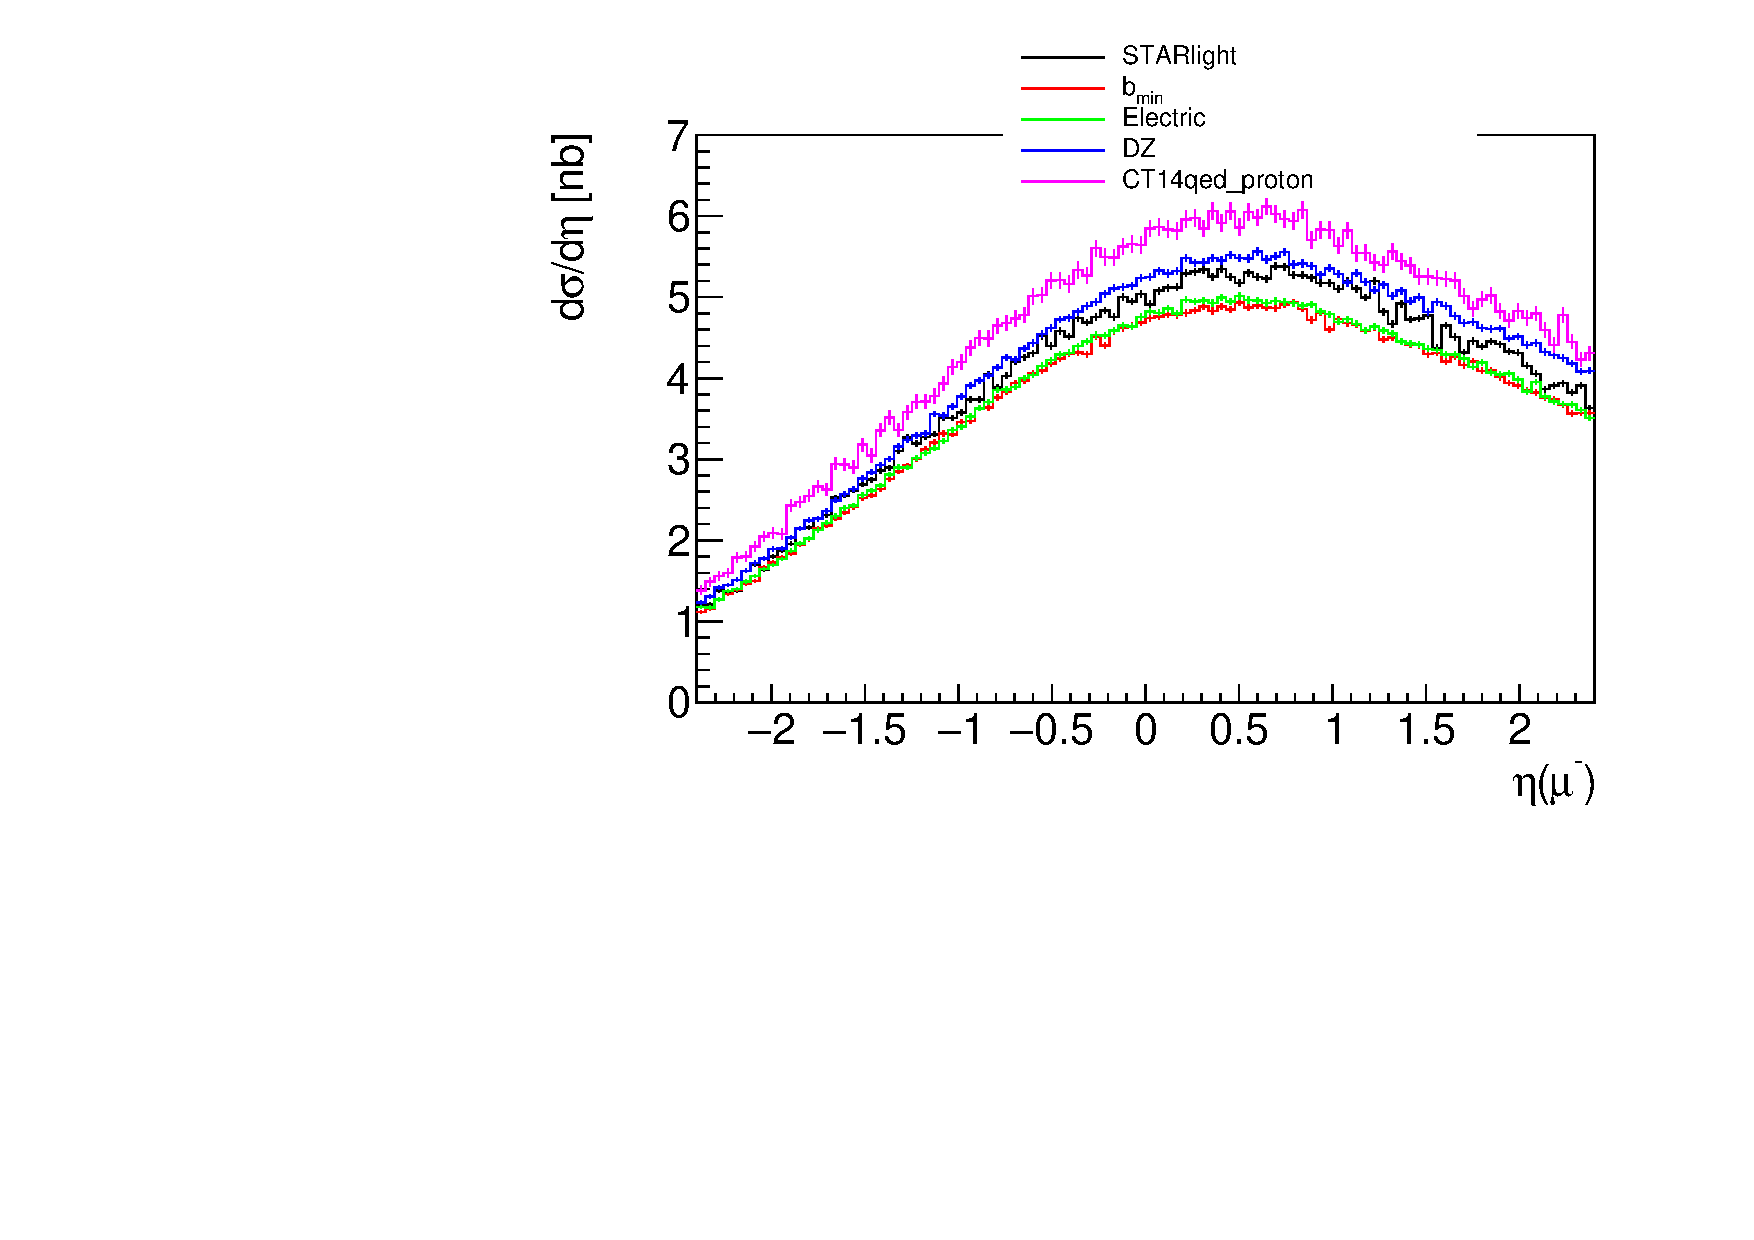
\includegraphics[width=0.4\textwidth]{figures/etal_elastic_cut.pdf}
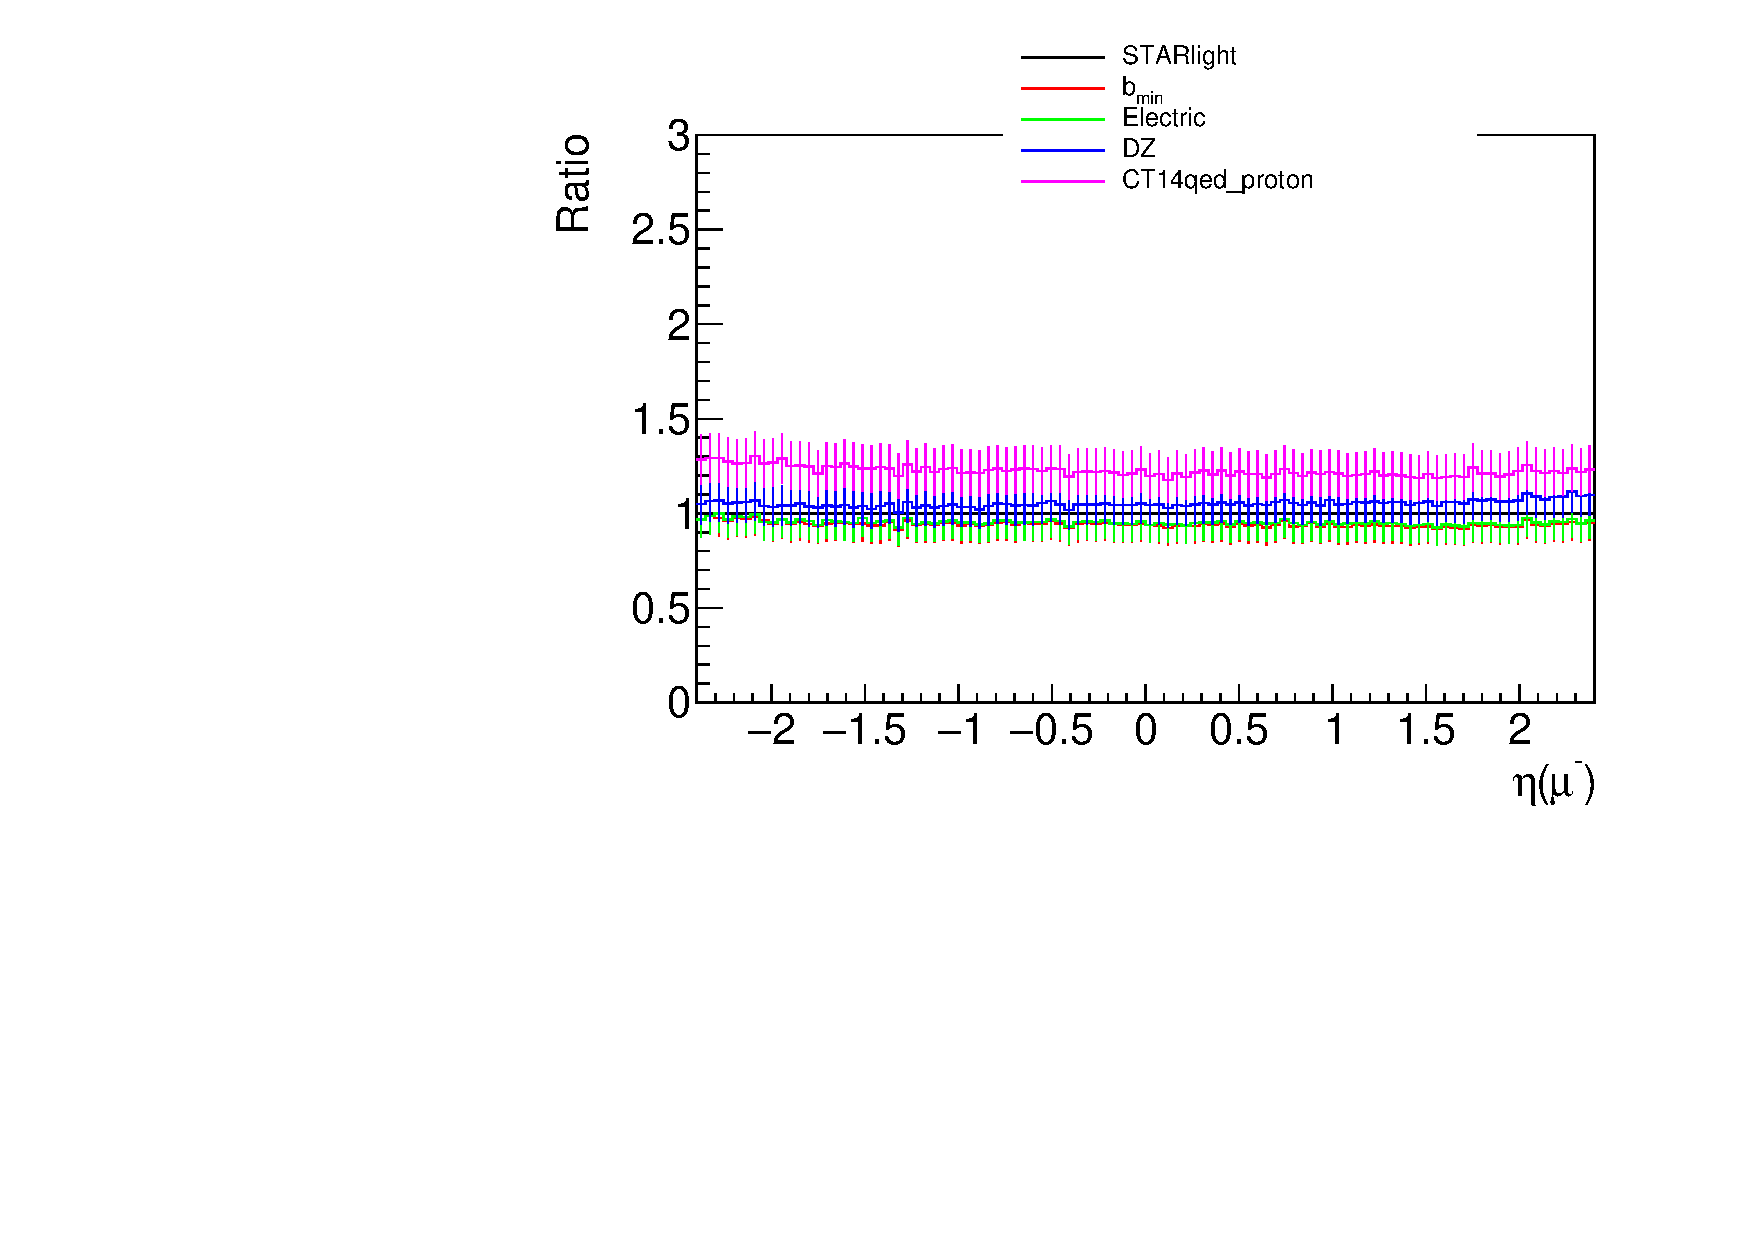
\includegraphics[width=0.4\textwidth]{figures/Ratioetal_elastic_cut.pdf}
\caption{Elastic distributions (fiducial region)}
\label{fig:elastic_cut}
\end{figure}

\begin{figure}[h!]
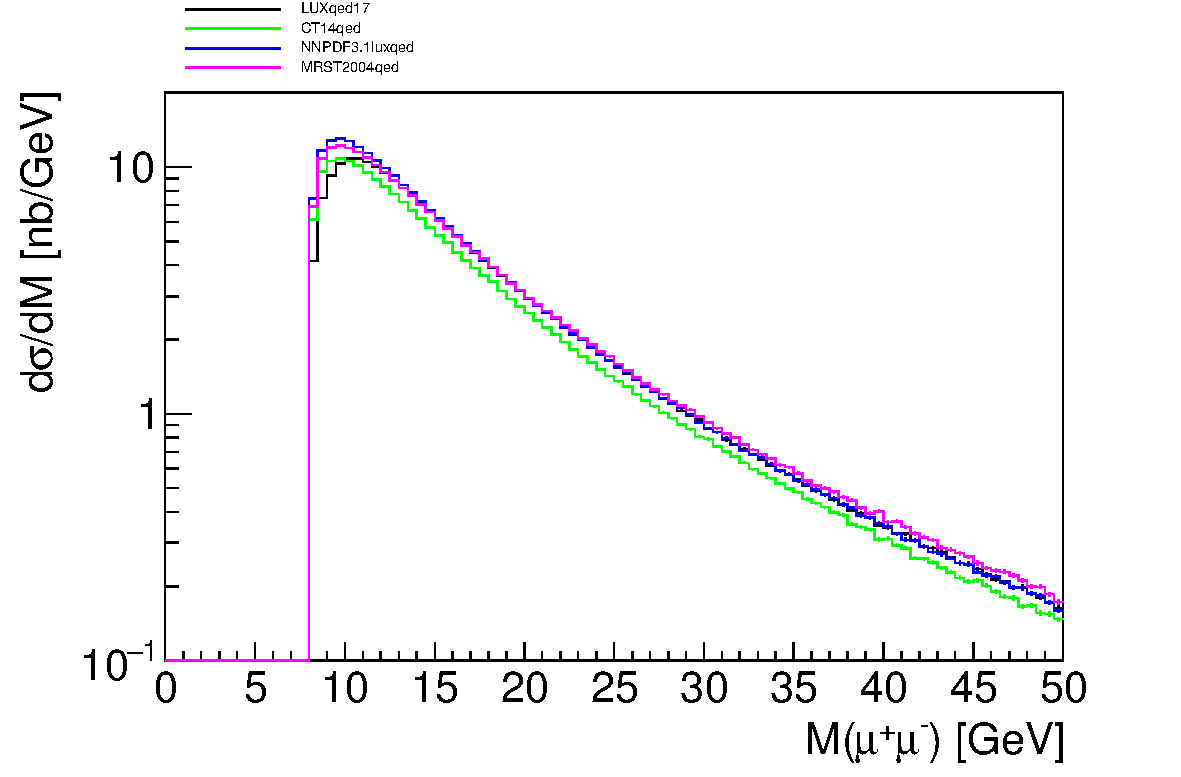
\includegraphics[width=0.4\textwidth]{figures/Mll_inc.pdf}
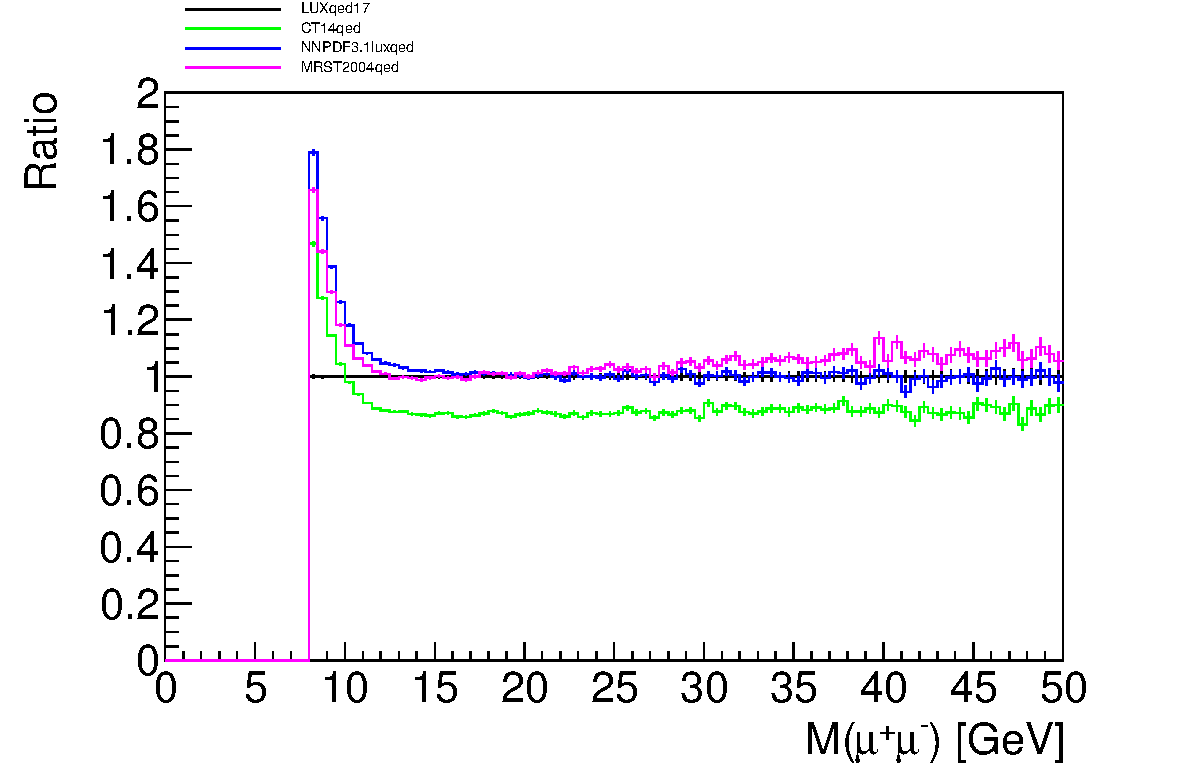
\includegraphics[width=0.4\textwidth]{figures/RatioMll_inc.pdf}
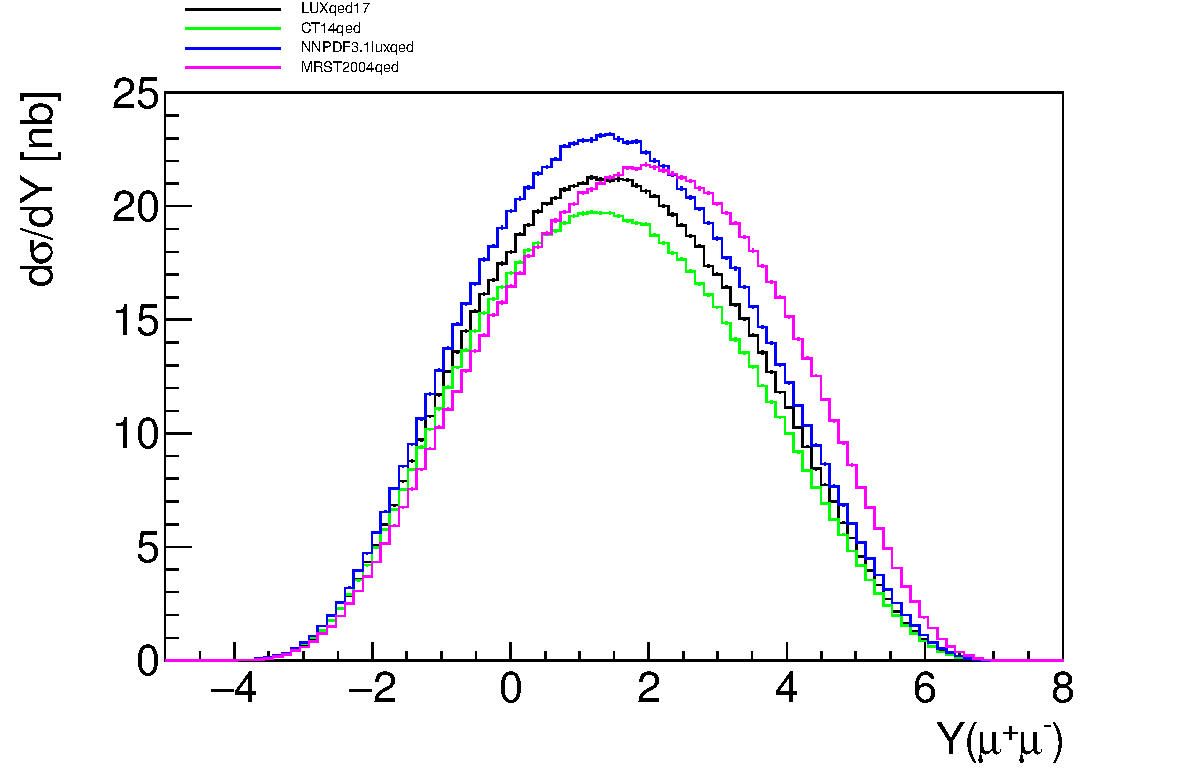
\includegraphics[width=0.4\textwidth]{figures/Yll_inc.pdf}
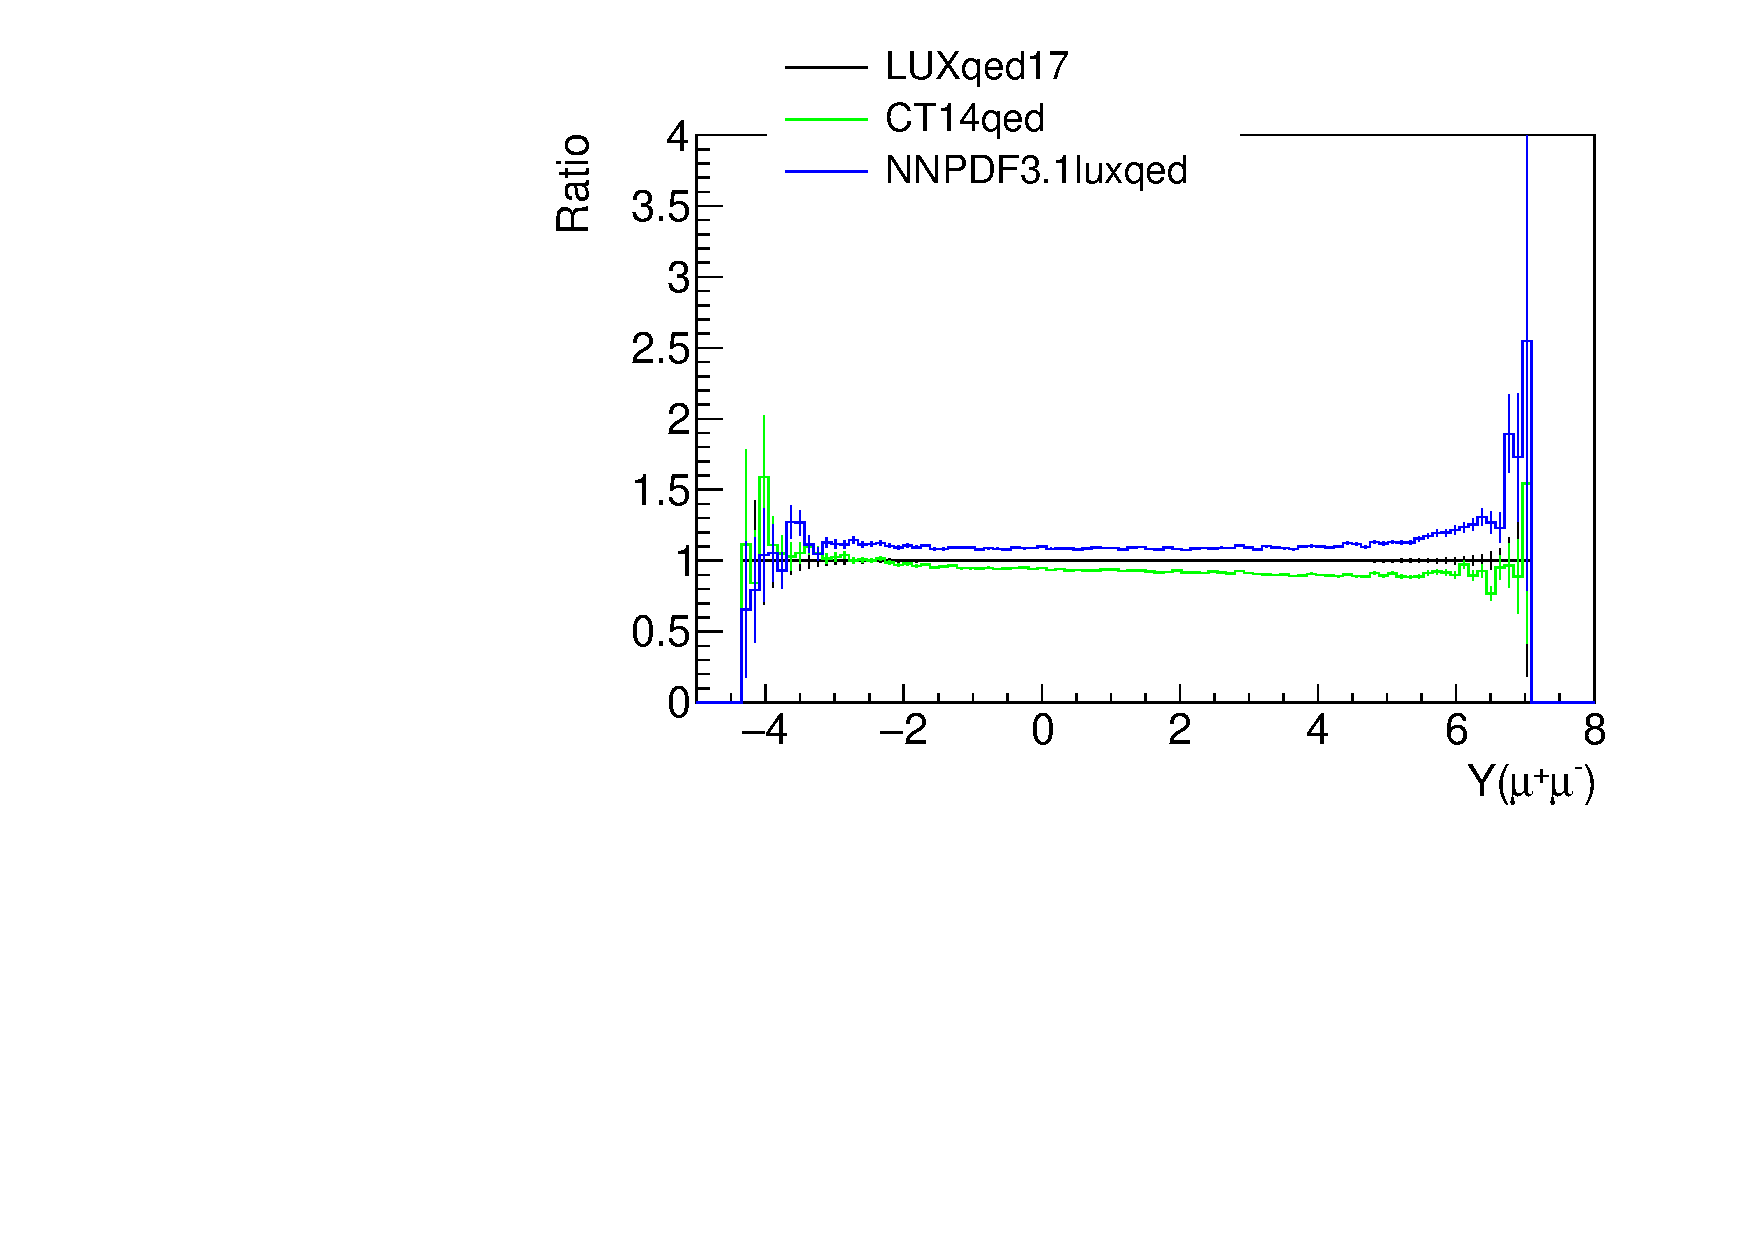
\includegraphics[width=0.4\textwidth]{figures/RatioYll_inc.pdf}
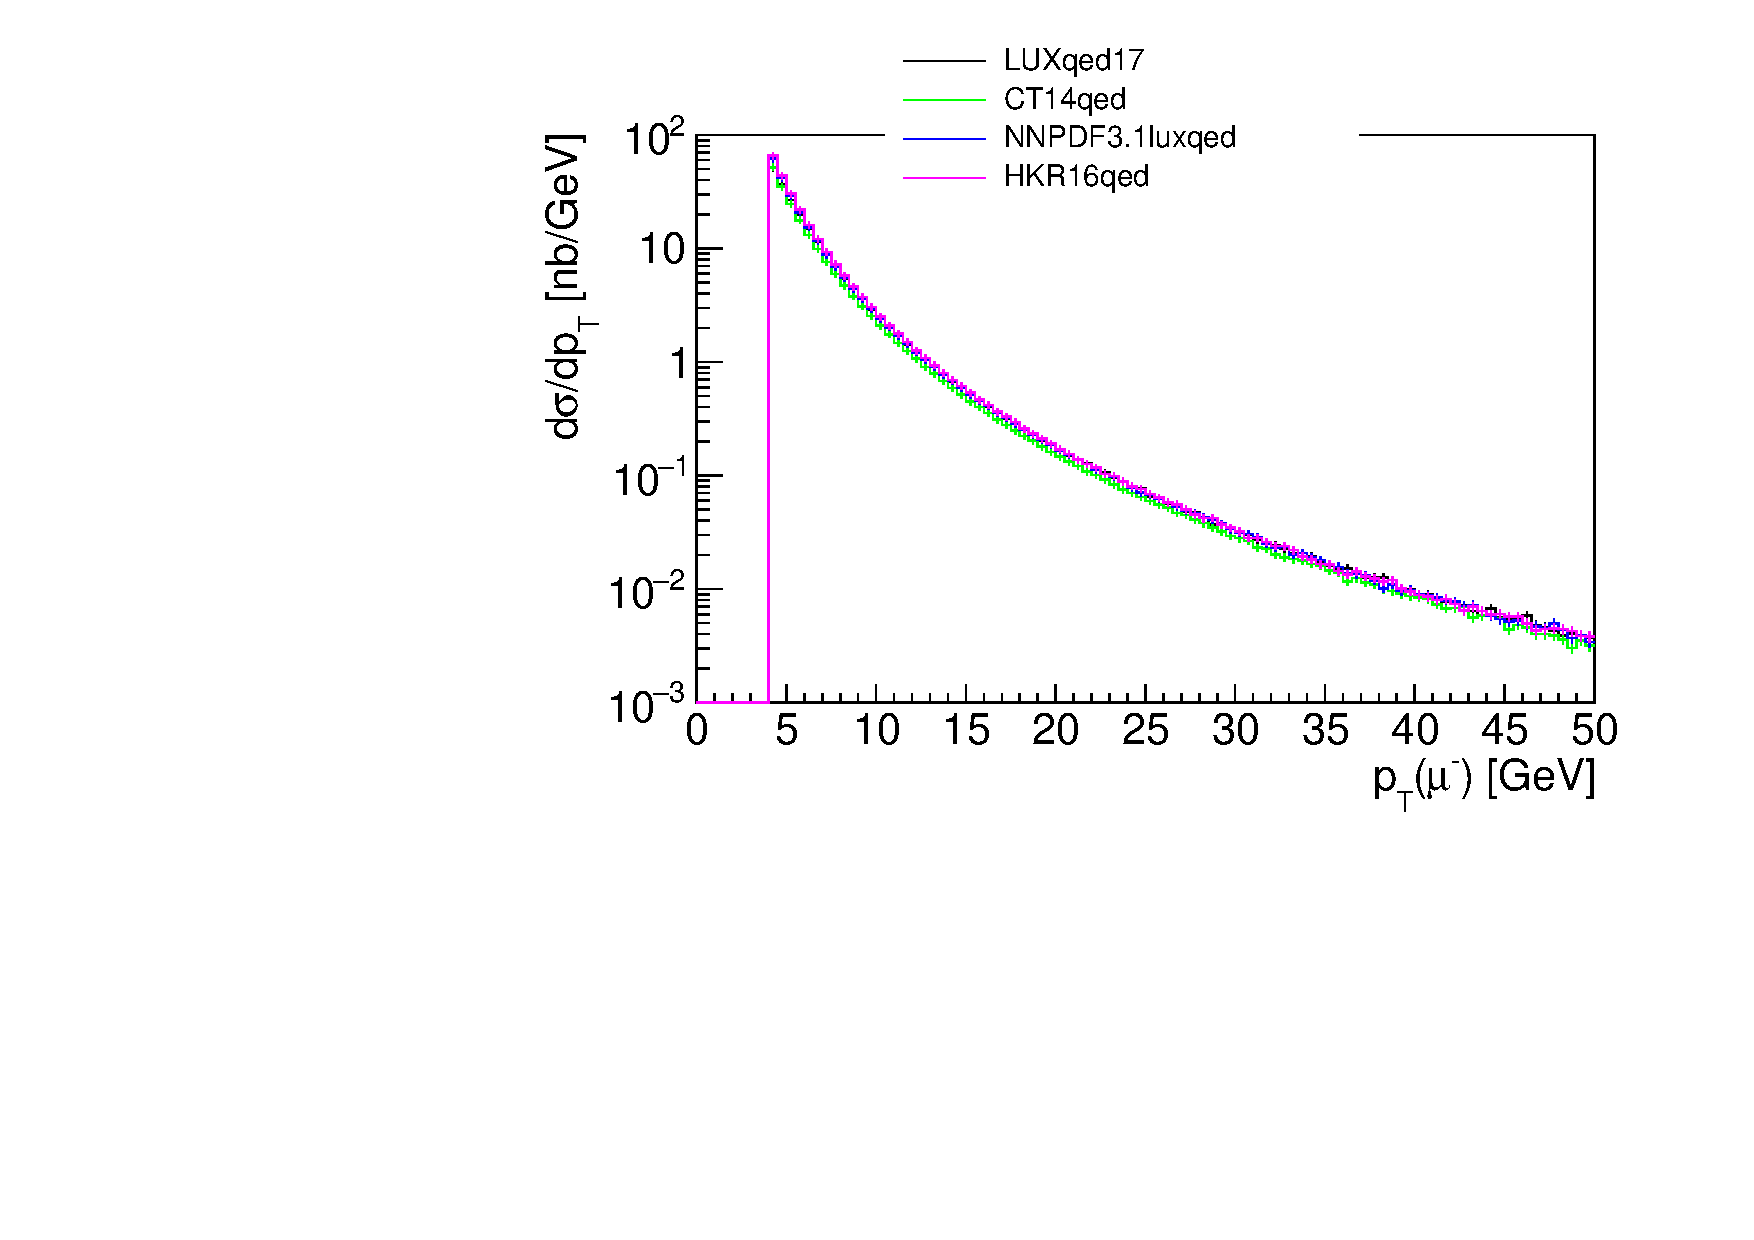
\includegraphics[width=0.4\textwidth]{figures/pTl_inc.pdf}
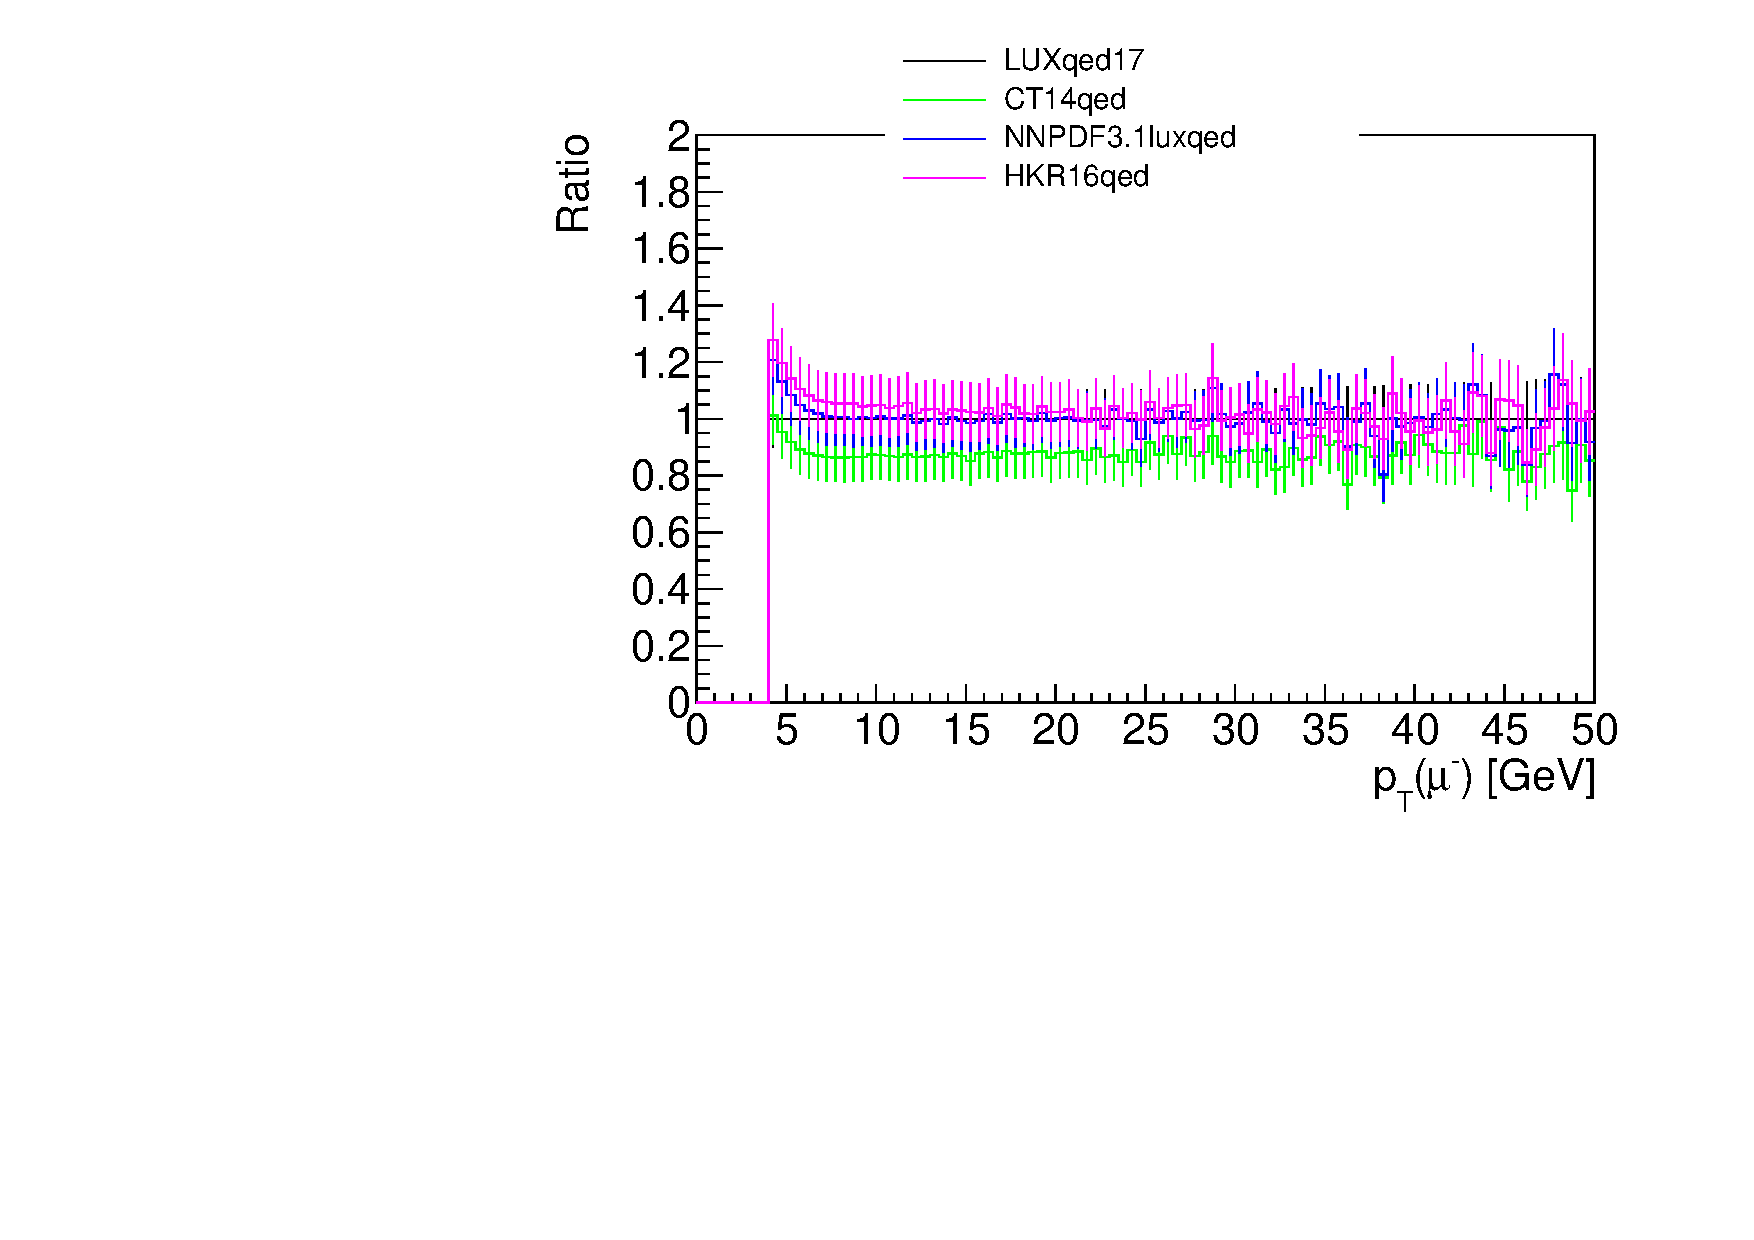
\includegraphics[width=0.4\textwidth]{figures/RatiopTl_inc.pdf}
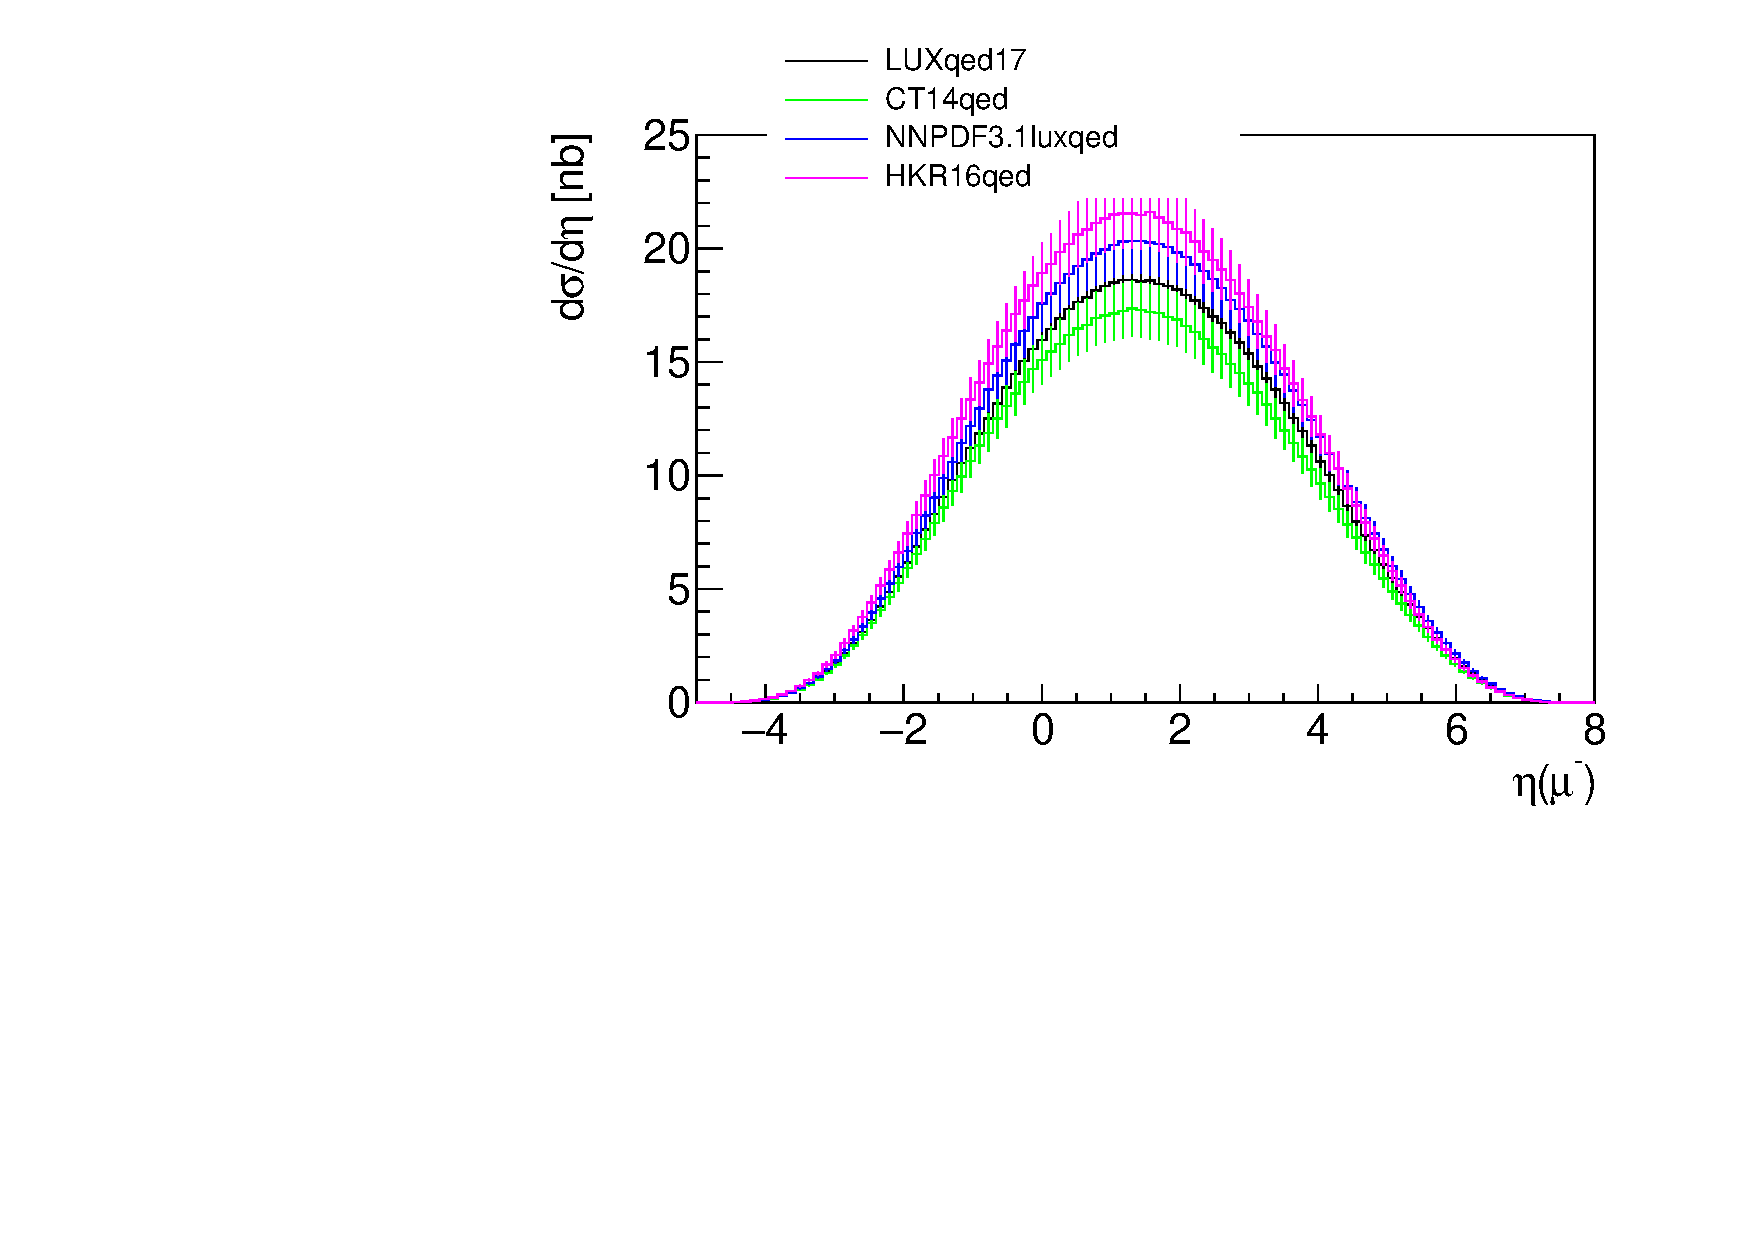
\includegraphics[width=0.4\textwidth]{figures/etal_inc.pdf}
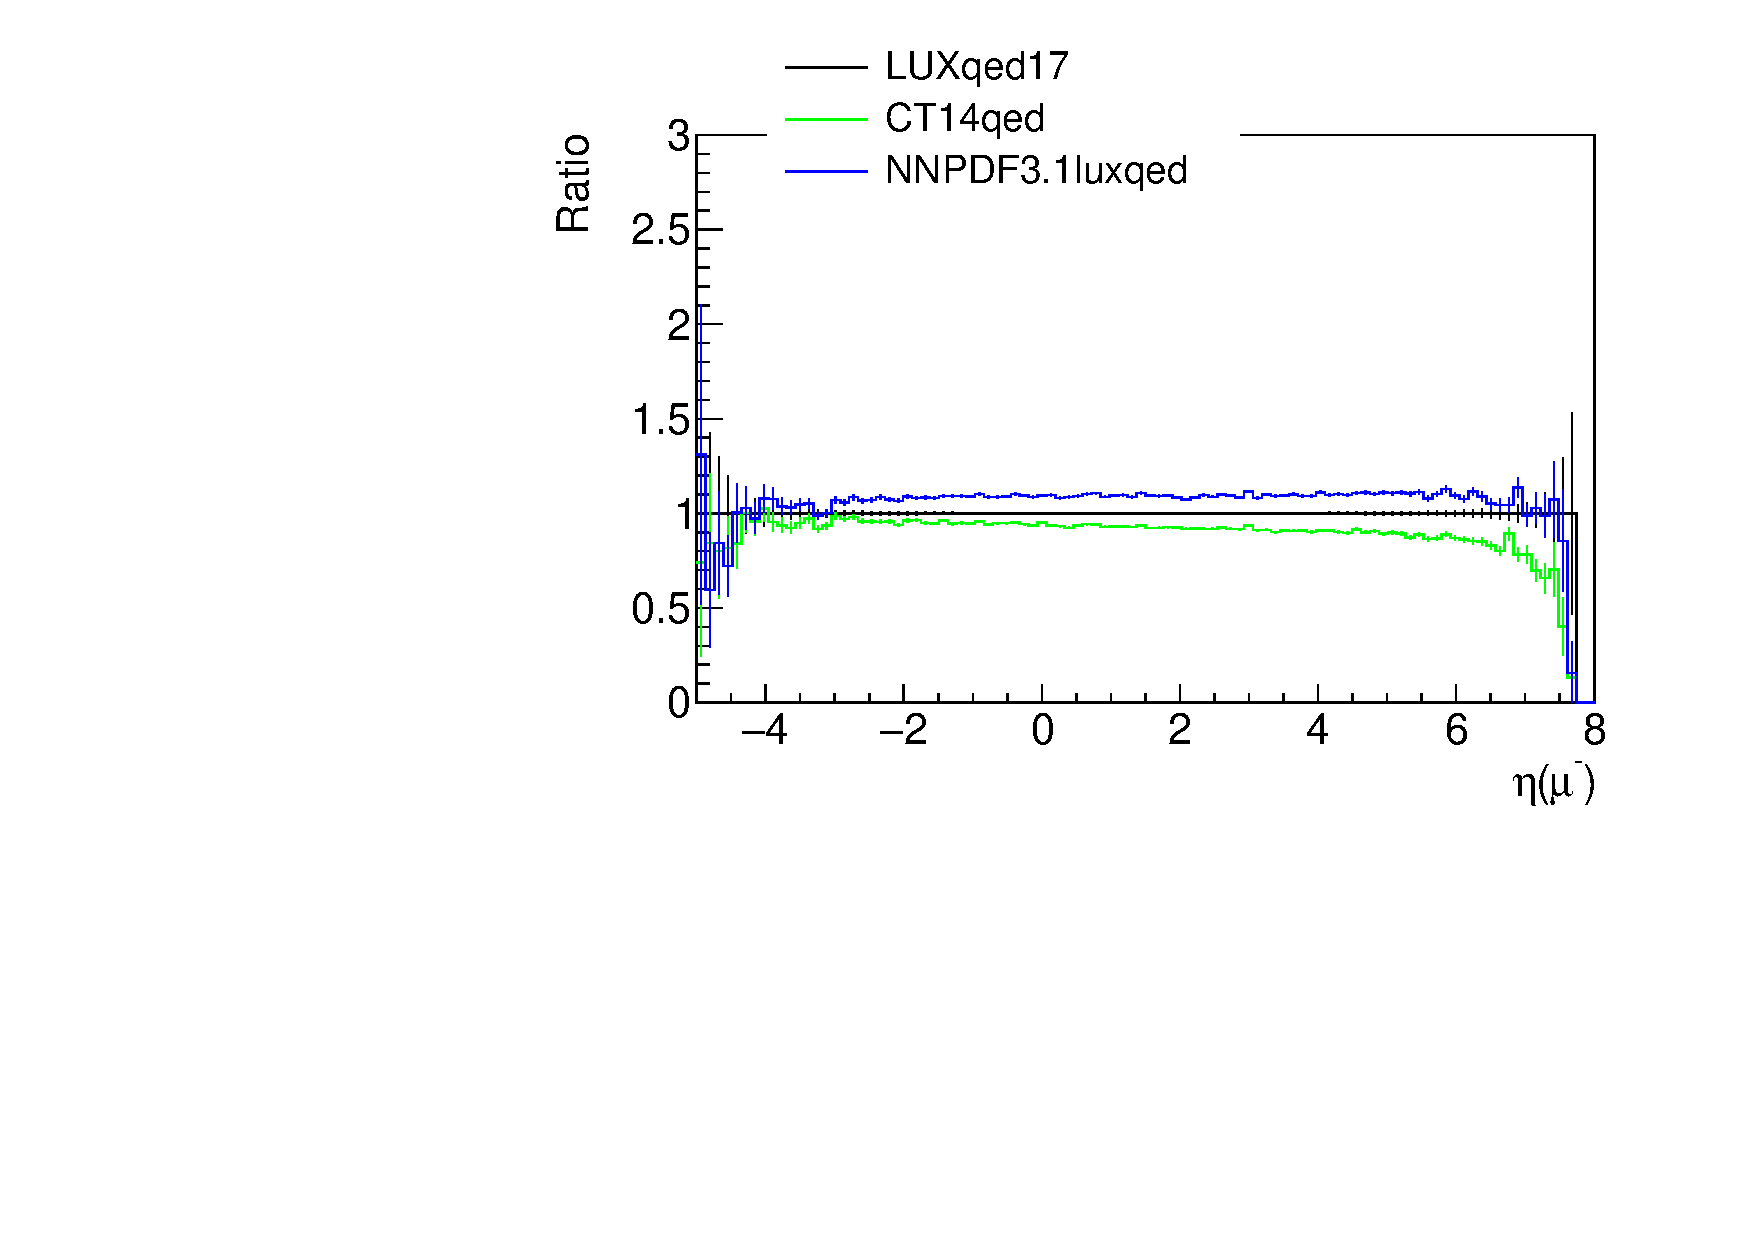
\includegraphics[width=0.4\textwidth]{figures/Ratioetal_inc.pdf}
\caption{Inclusive distributions (the only cut is on leptons $p_T$)}
\label{fig:inc}
\end{figure}

\begin{figure}[h!]
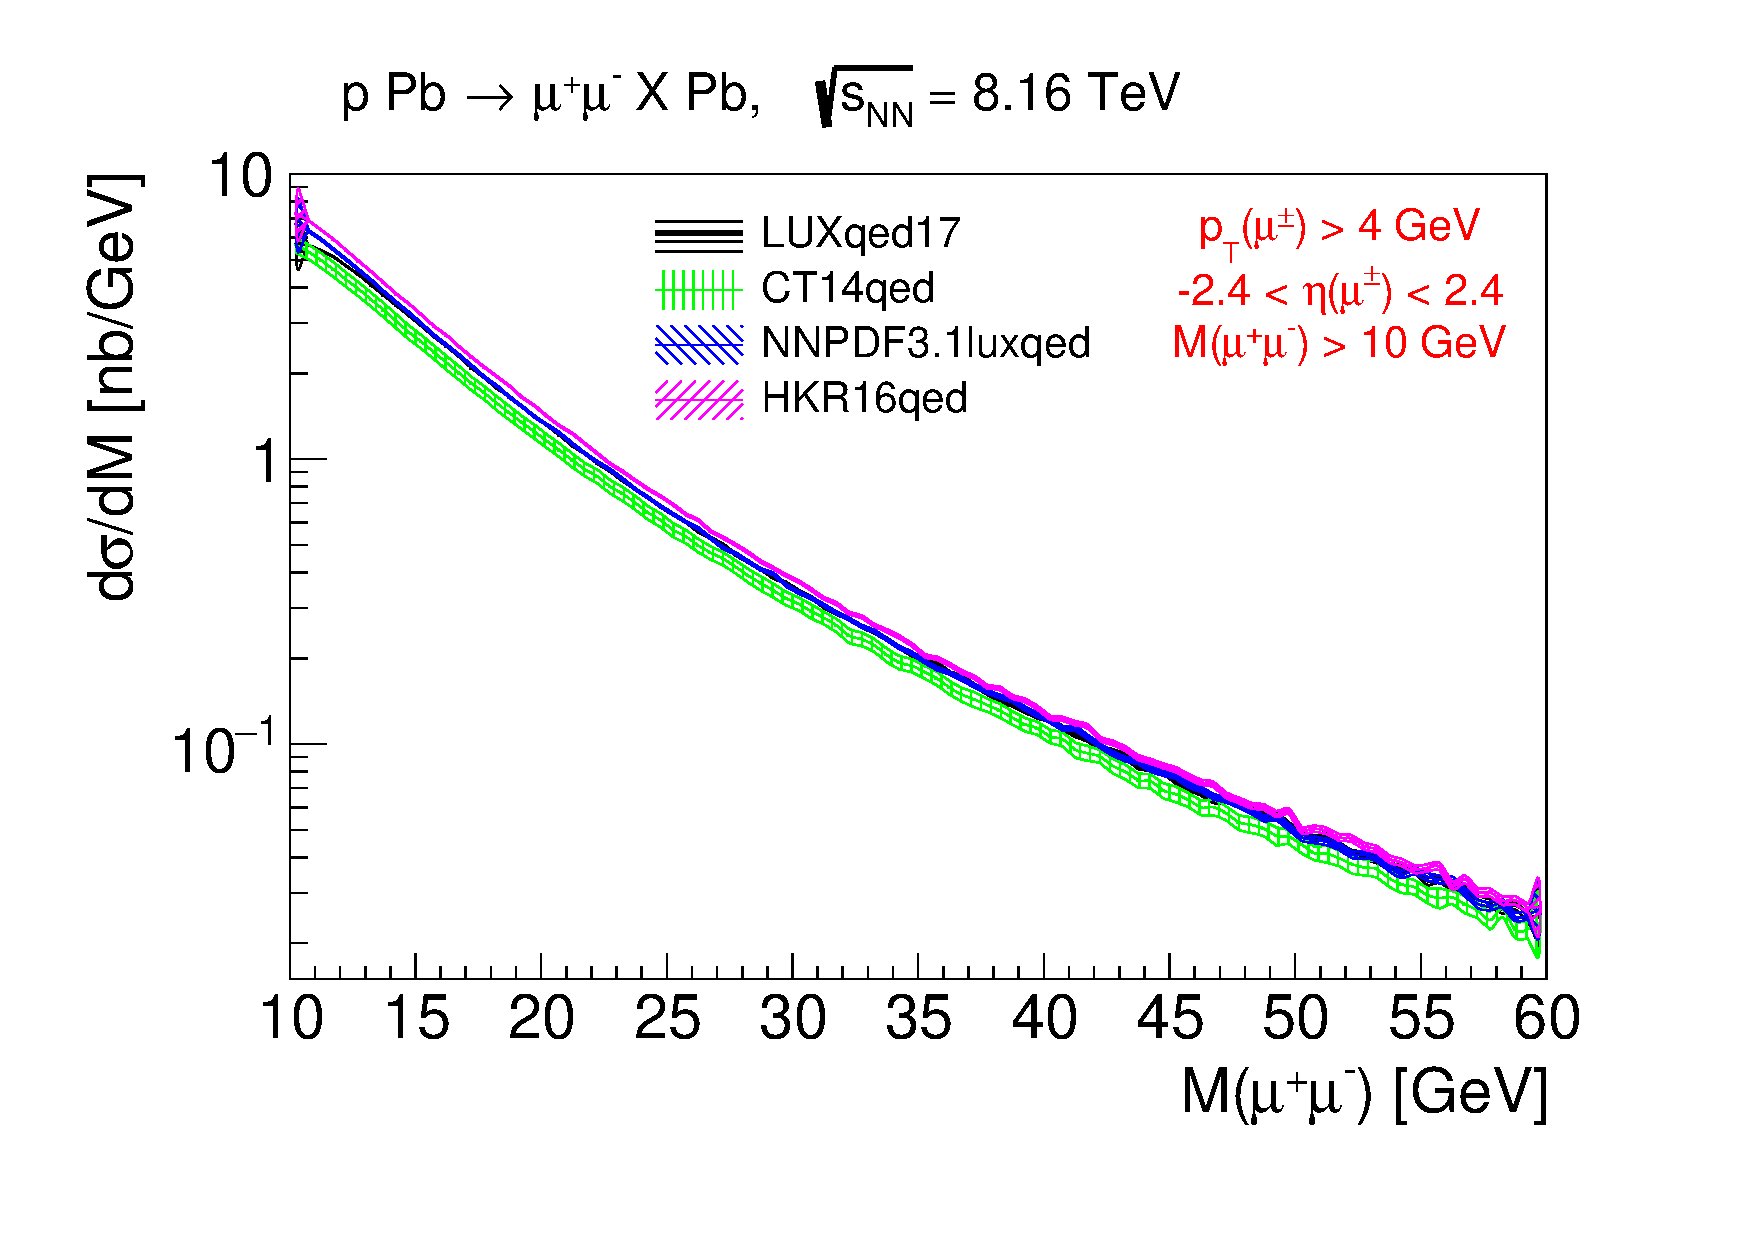
\includegraphics[width=0.4\textwidth]{figures/Mll_inc_cut.pdf}
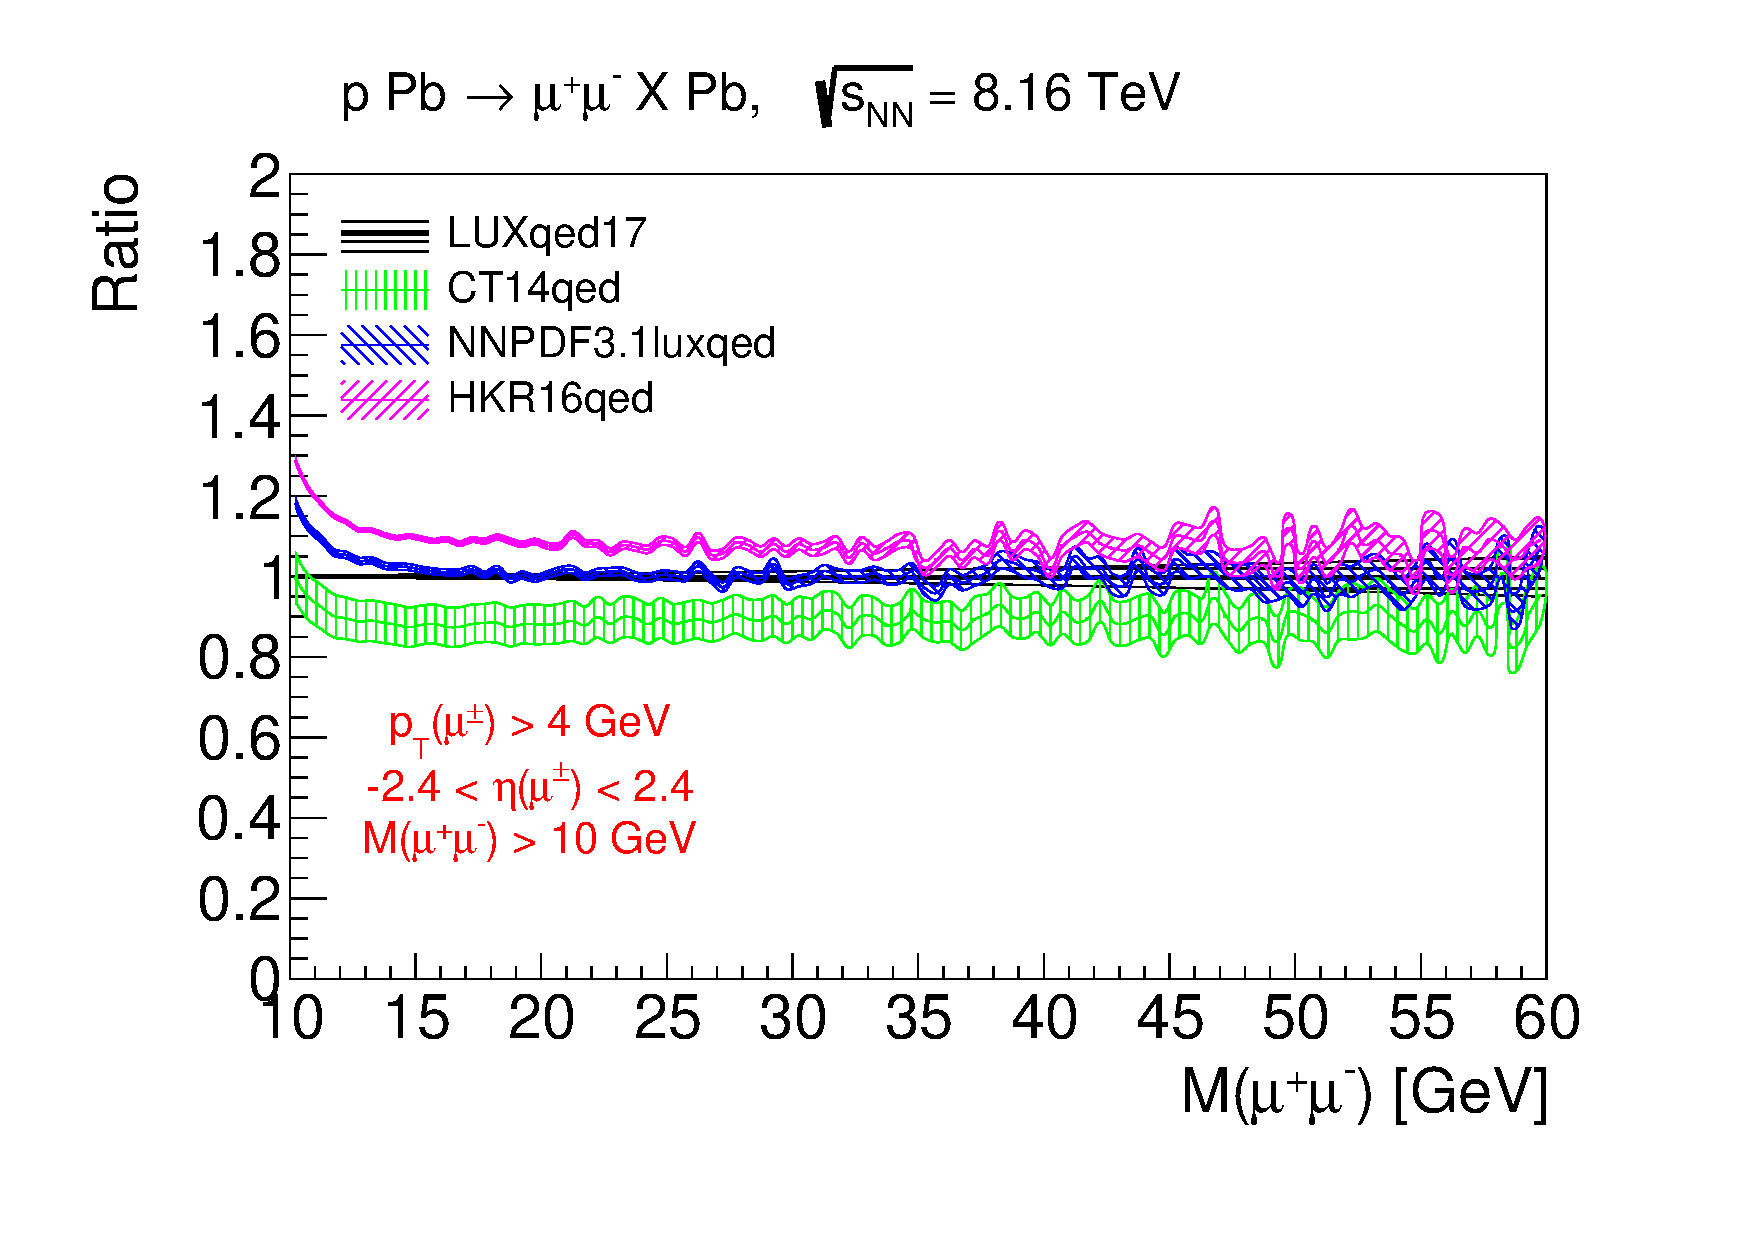
\includegraphics[width=0.4\textwidth]{figures/RatioMll_inc_cut.pdf}
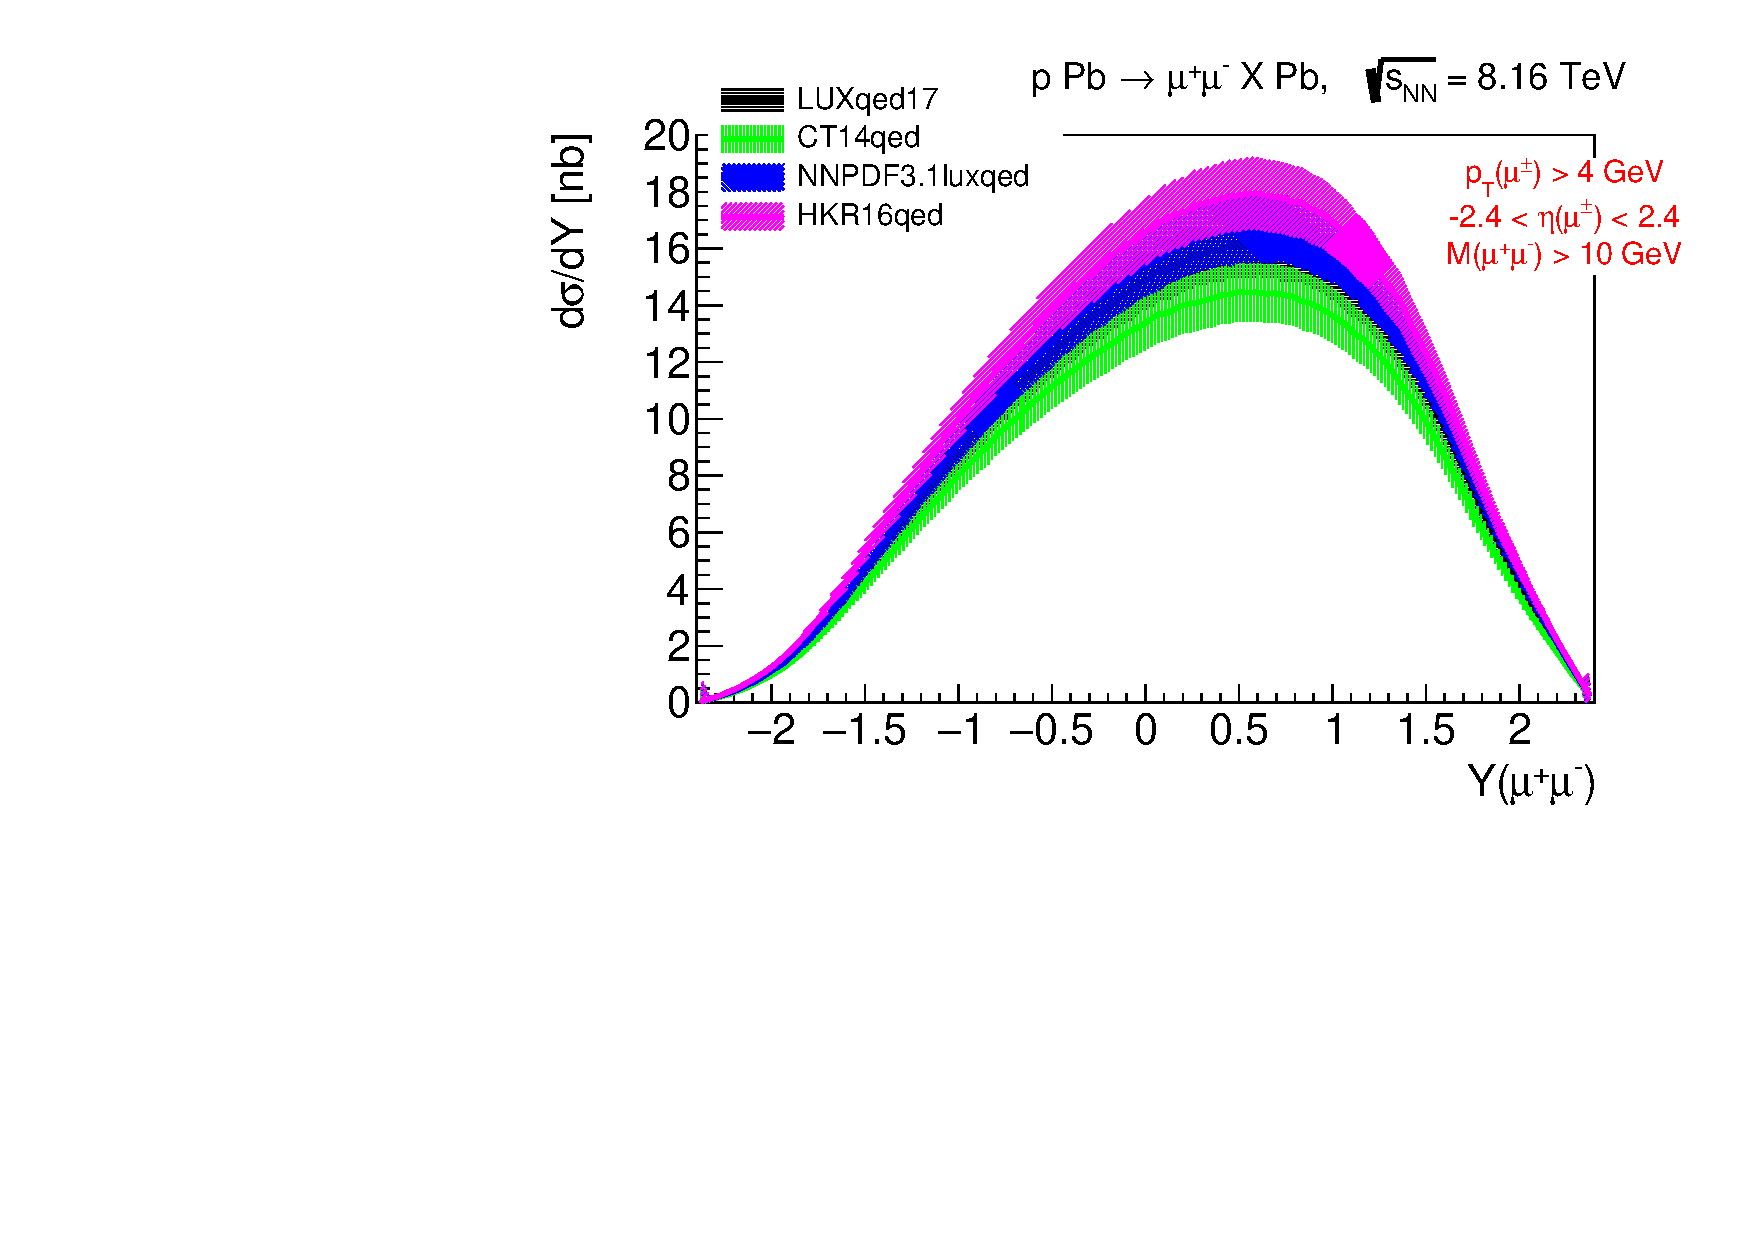
\includegraphics[width=0.4\textwidth]{figures/Yll_inc_cut.pdf}
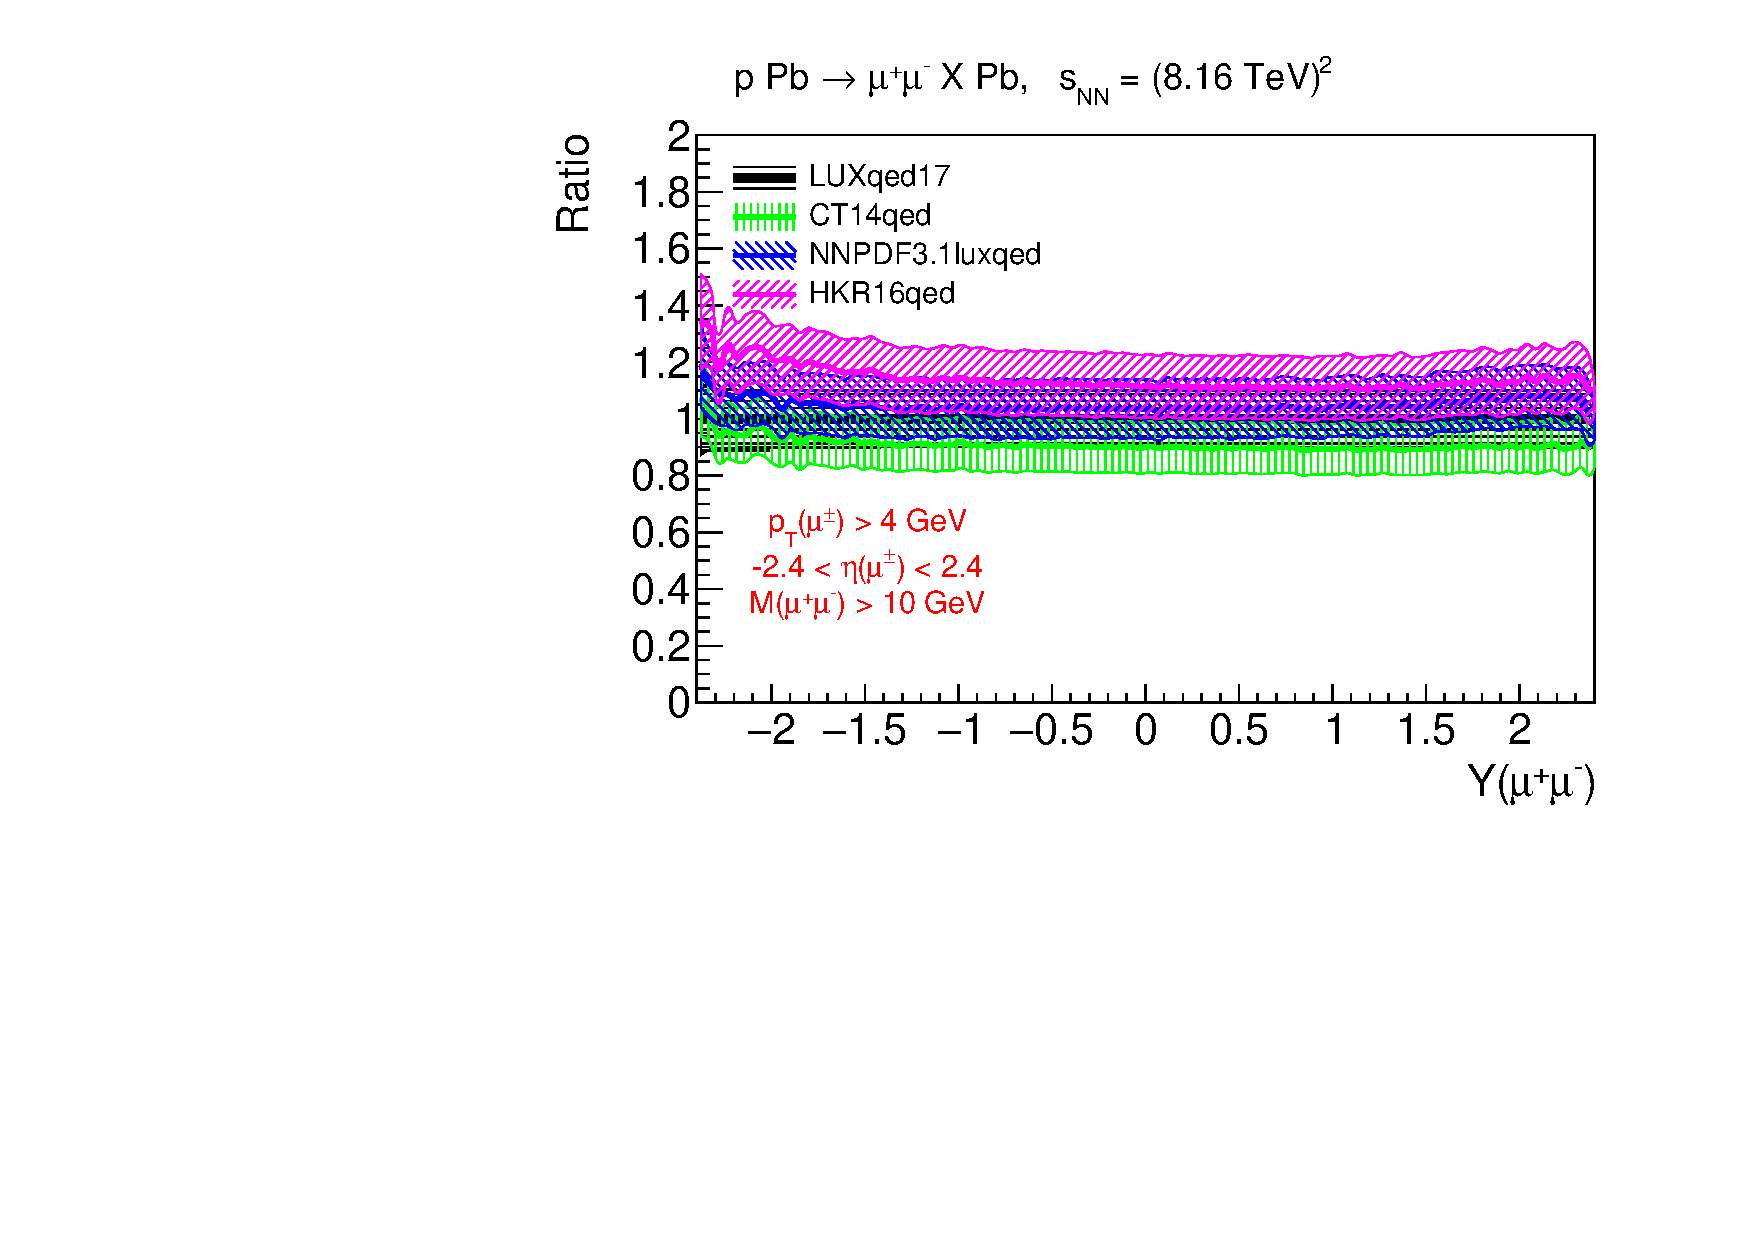
\includegraphics[width=0.4\textwidth]{figures/RatioYll_inc_cut.pdf}
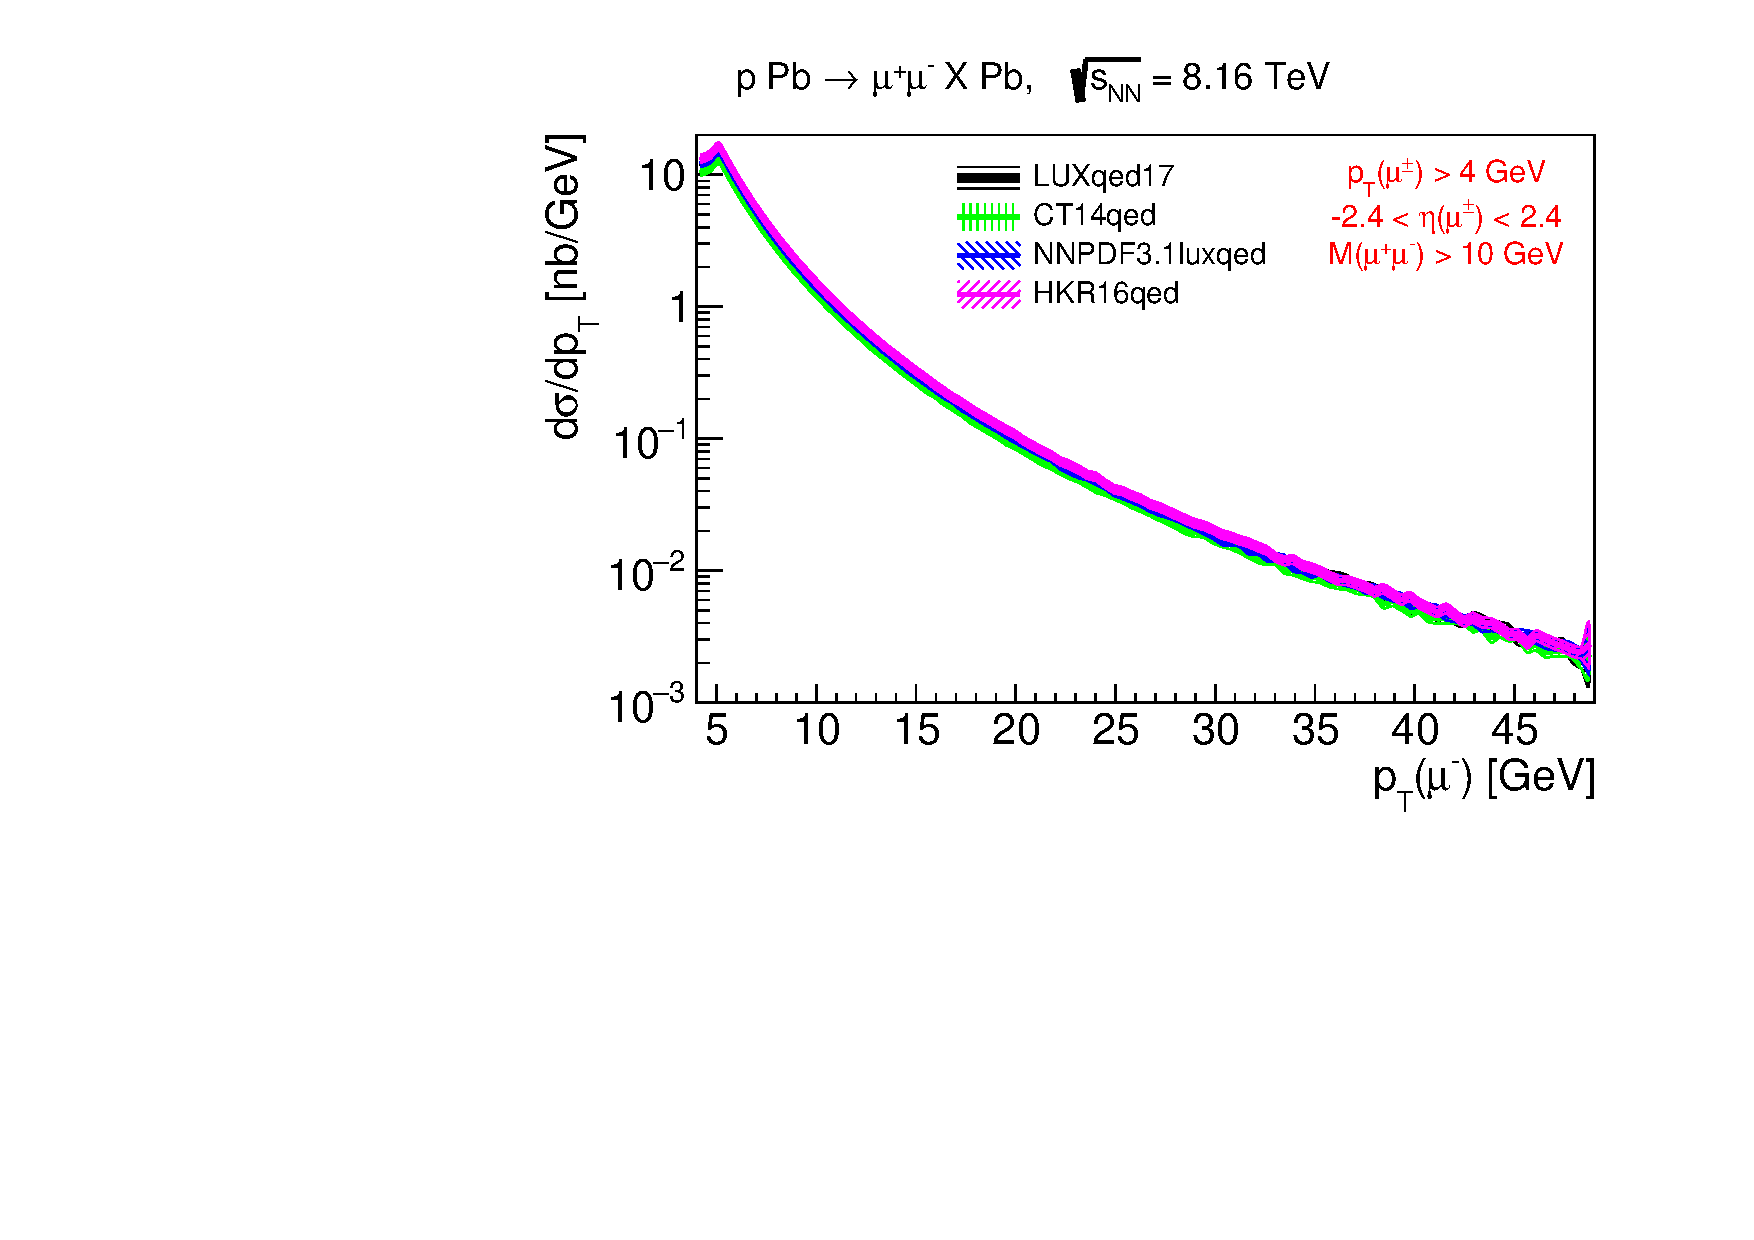
\includegraphics[width=0.4\textwidth]{figures/pTl_inc_cut.pdf}
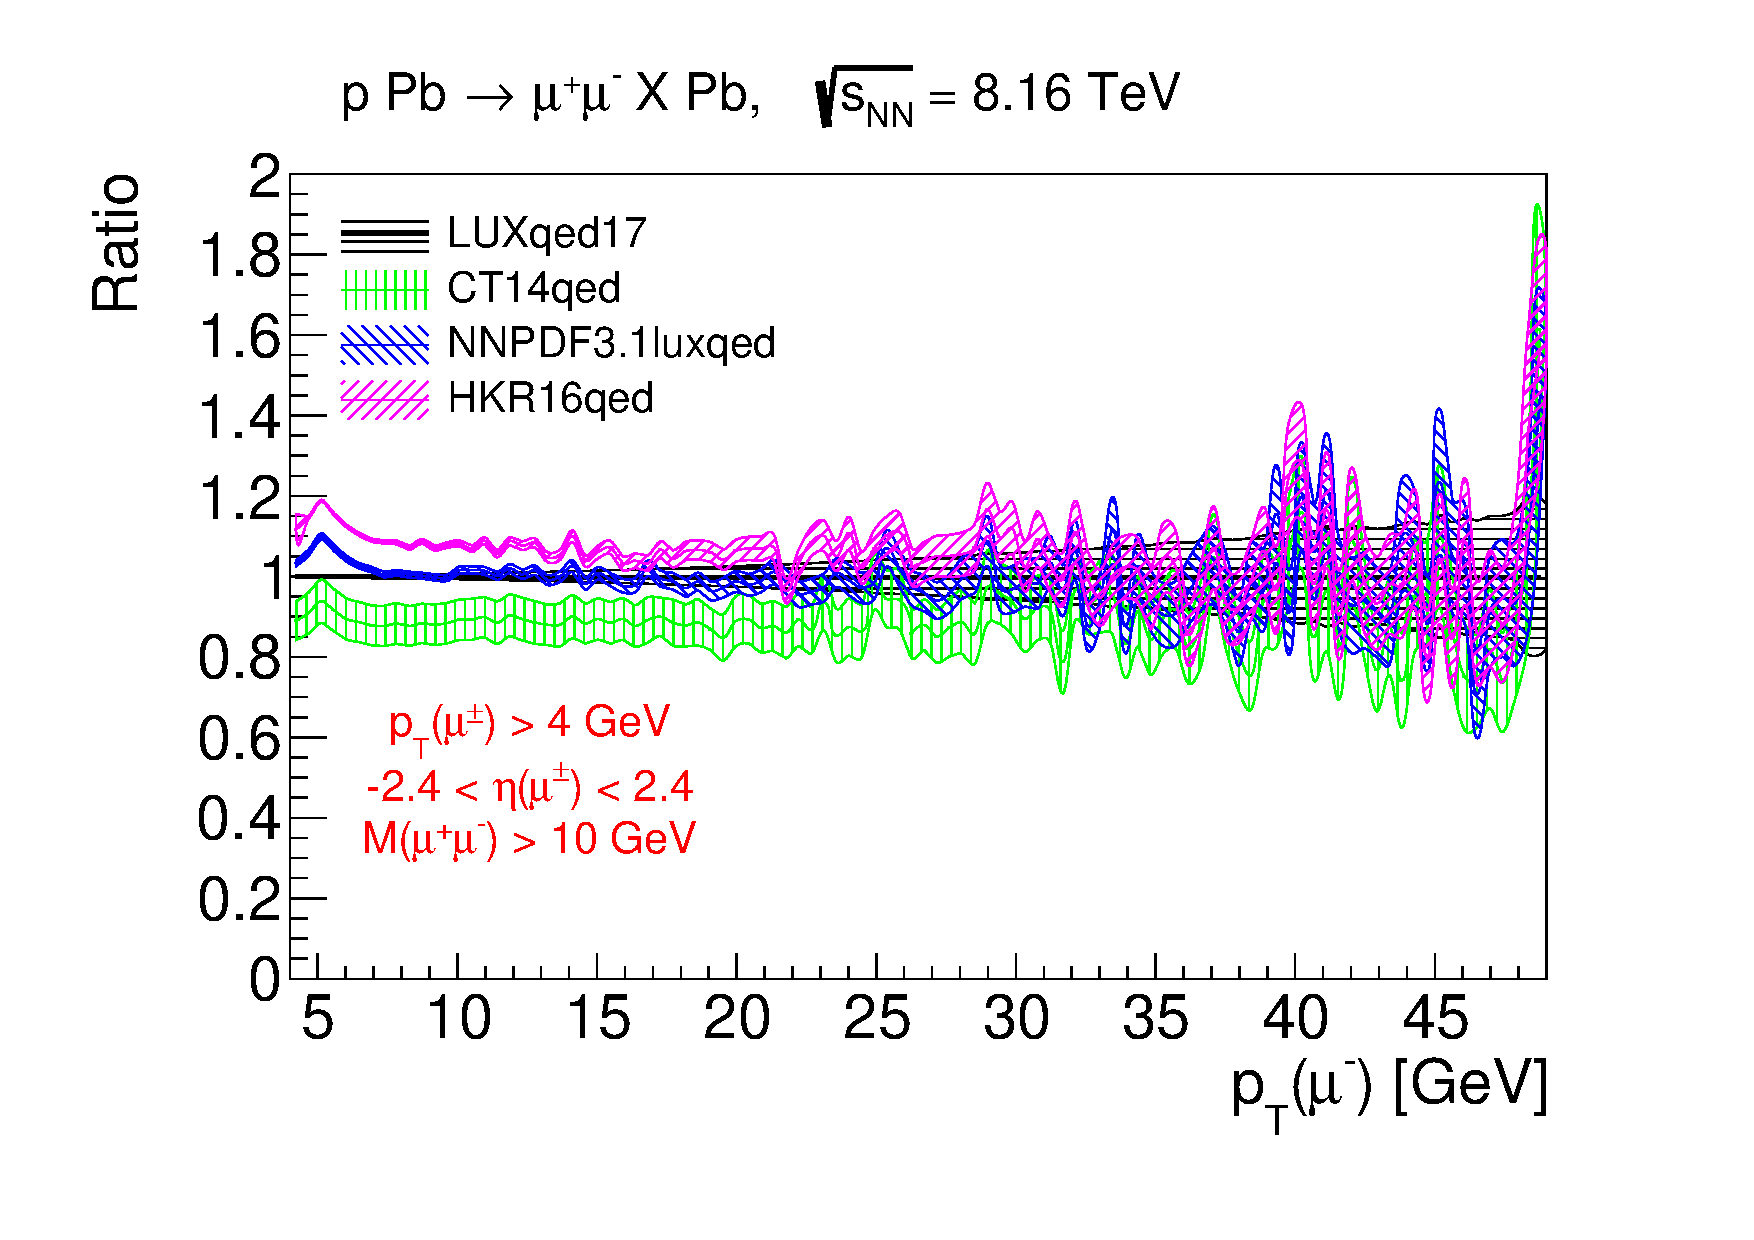
\includegraphics[width=0.4\textwidth]{figures/RatiopTl_inc_cut.pdf}
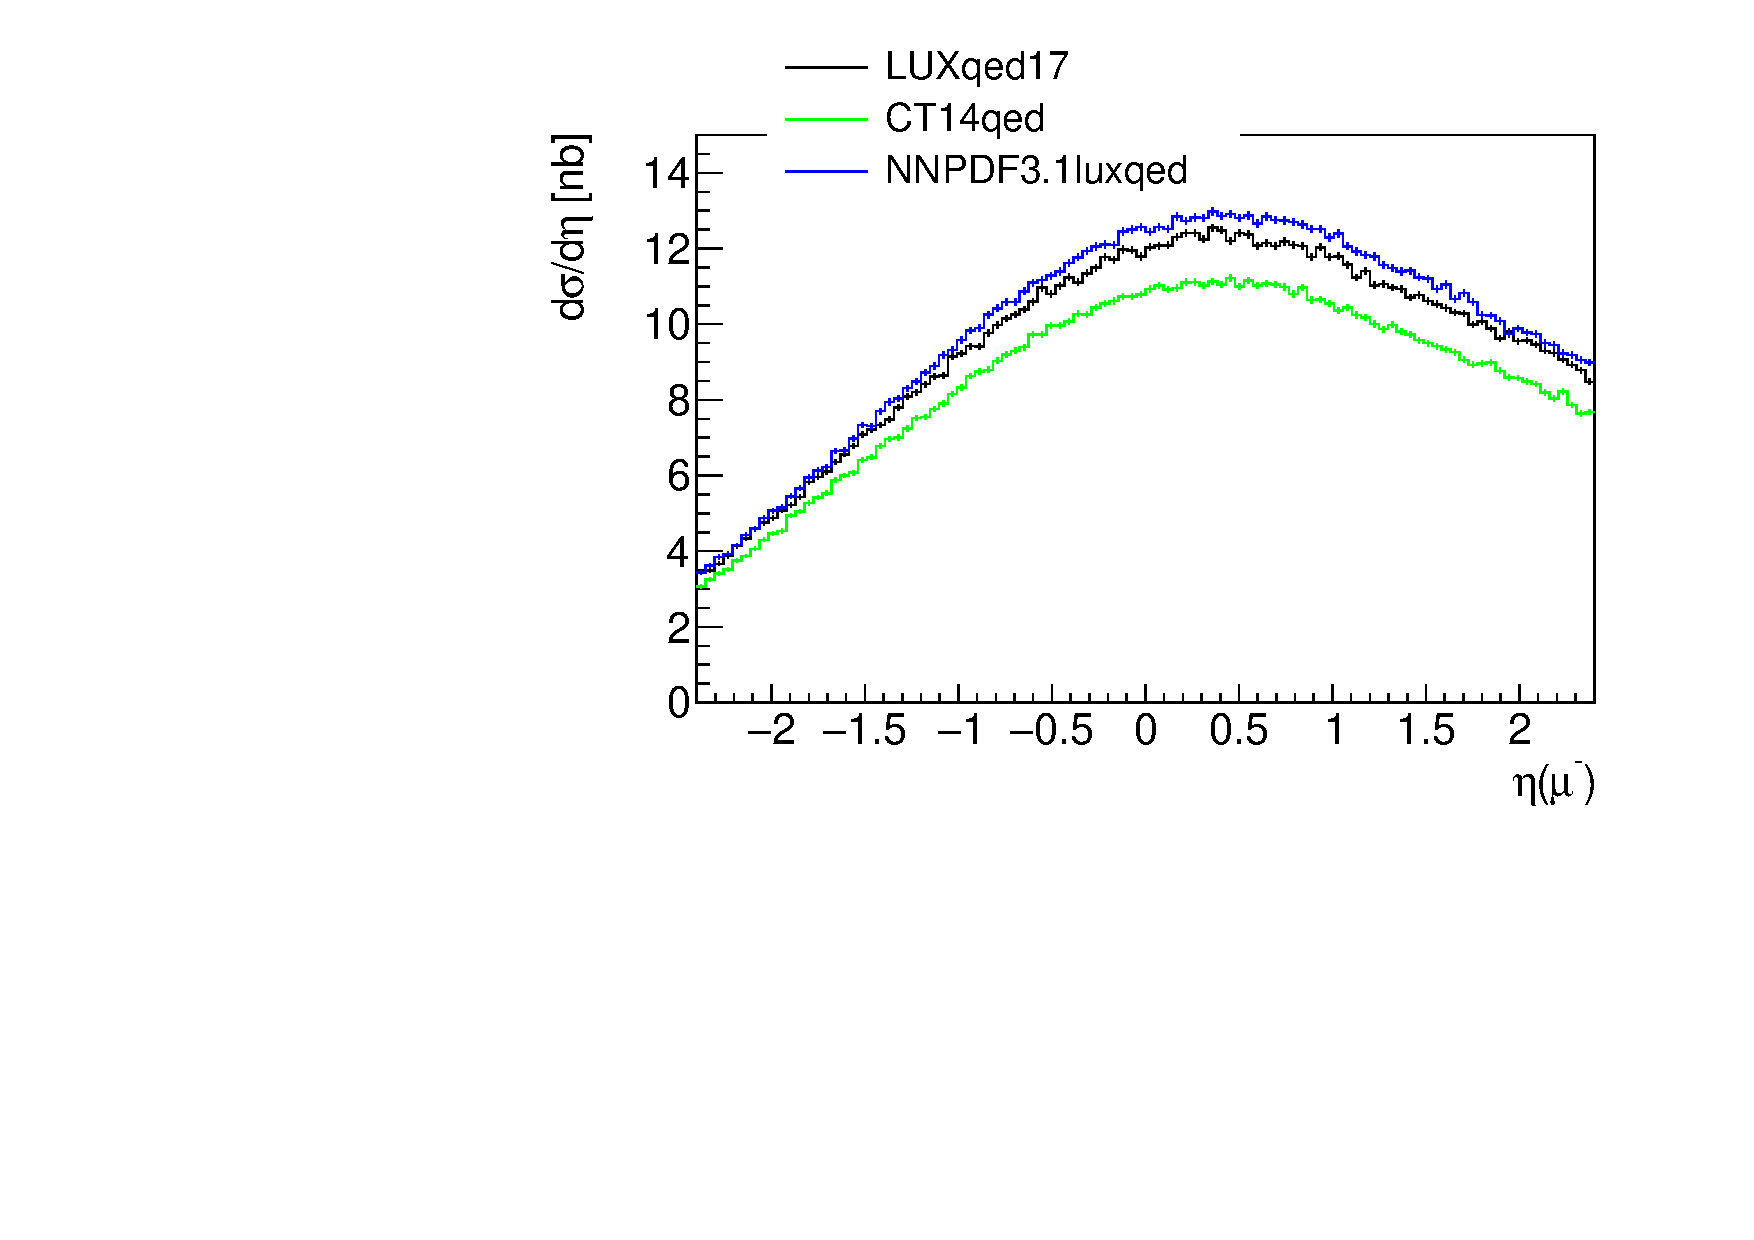
\includegraphics[width=0.4\textwidth]{figures/etal_inc_cut.pdf}
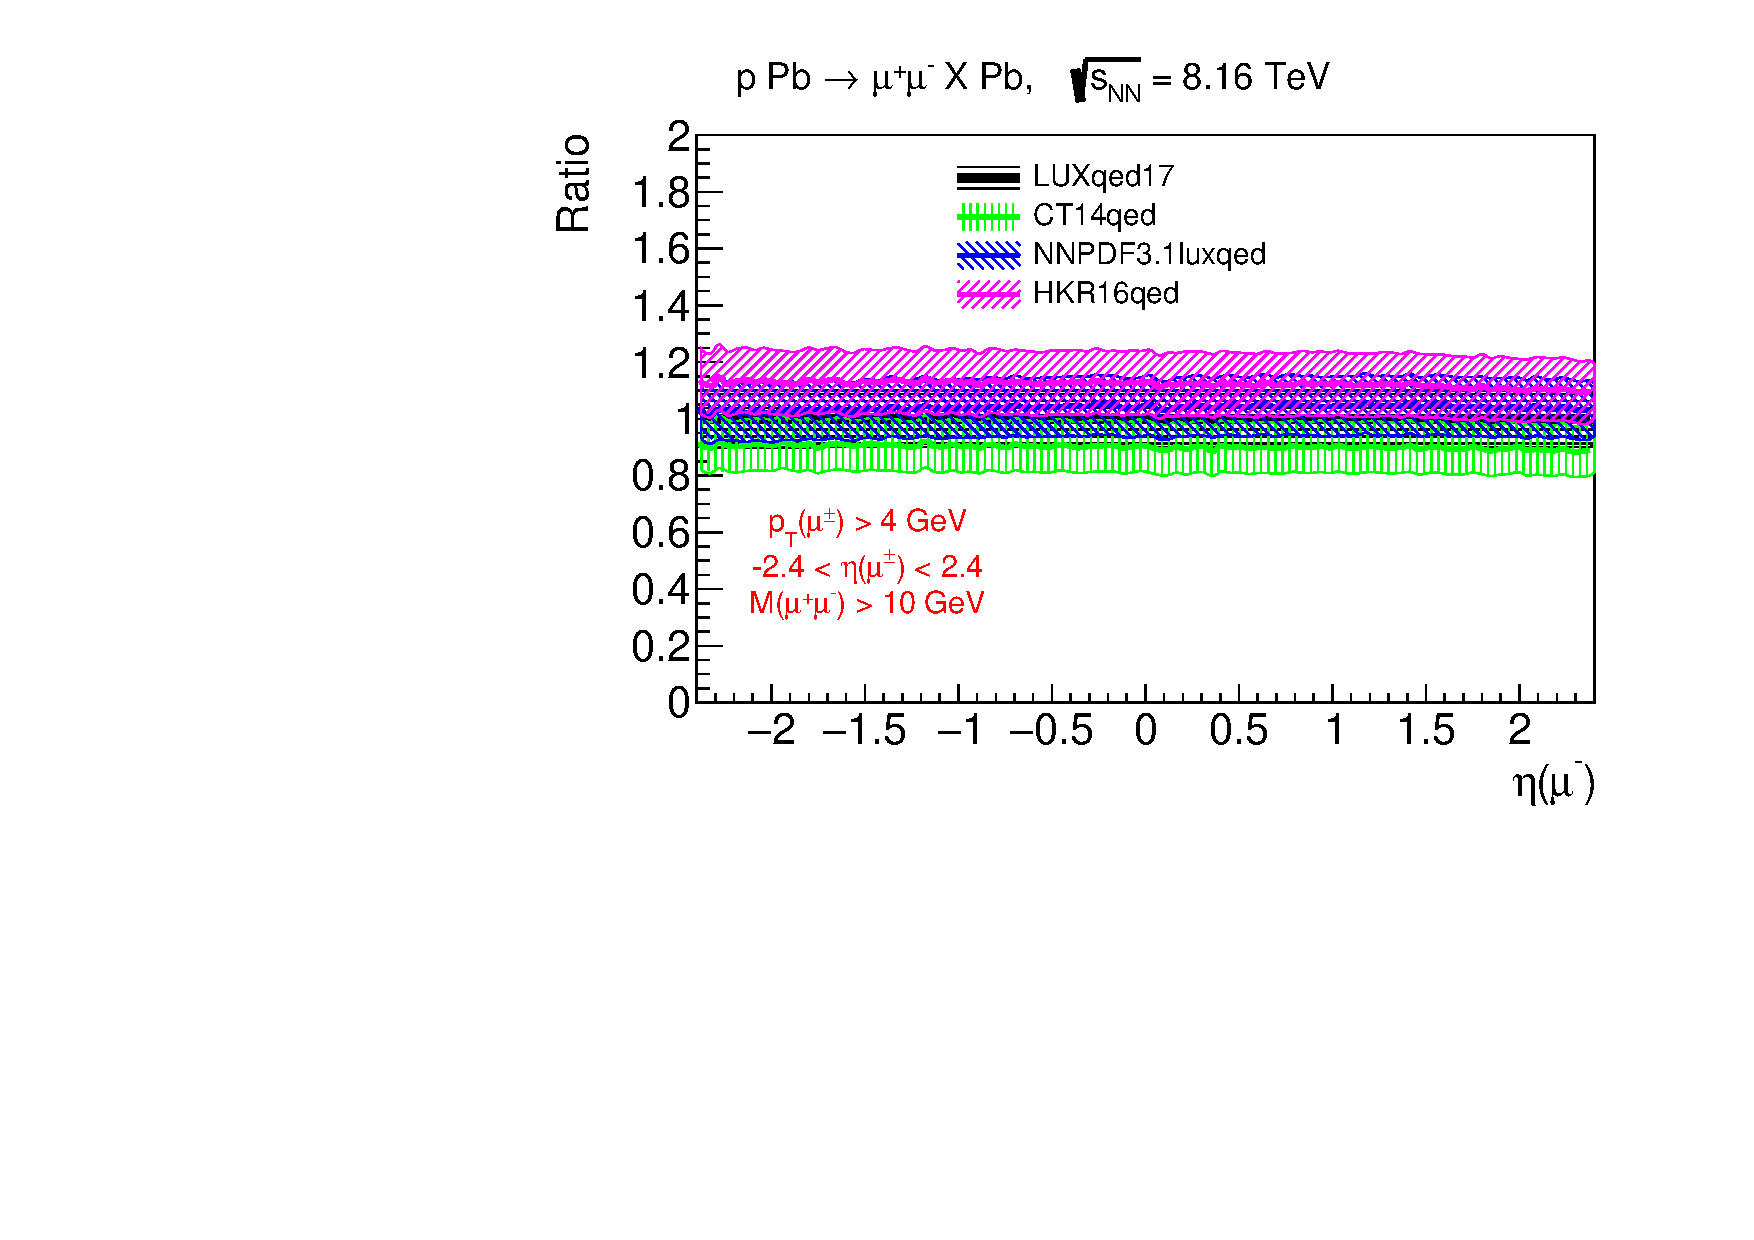
\includegraphics[width=0.4\textwidth]{figures/Ratioetal_inc_cut.pdf}
\caption{Inclusive distributions (fiducial regoin)}
\label{fig:inc_cut}
\end{figure}

The integrated fiducial cross-sections are summarized in Tab.~\ref{}.

(some discussion here...)

It should be made clear, that the calculations with collinear photons (at lowest order) produce leptons that are back-to-back in transverse kinematics. Therefore, to take the effect of inelastic photon virtuality into account, a dedicated parton shower algorithm should be used.

(mention we don't want to do extra PS; we would rather stick to kt factorization)

%%%%%%%%%%%%%%%%%%%%%%%%%%%%%%%%%%
\section{Results using $k_T$-factorization approach}
%%%%%%%%%%%%%%%%%%%%%%%%%%%%%%%%%%
%------------------------------------------------------------------------------------

%-------------------------------------------------------------------------------------------
%\subsection{Structure functions as input for unintegrated fluxes}
%-------------------------------------------------------------------------------------------

Several different parametrizations of proton strucure functions are used. Those are labeled as:
%%
\begin{itemize} 

 \item ALLM \cite{Abramowicz:1991xz,Abramowicz:1997ms}: This parametrization gives a good fit to $F_2$ in most of the measured regions.
   
%\item FJLLM \cite{Fiore:2002re}: This parametrization explicitly includes the nucleon resonances and provides very good descripton of the CLAS data~\cite{Osipenko:2003bu}.
  
\item SY \cite{Suri:1971yx}: This parameterization of Suri and Yennie from the early 1970's does not include DGLAP evolution. It is still  used as one of the defaults in the LPAIR event generator~\cite{Vermaseren:1982cz}.
    
\item SU \cite{Szczurek:1999rd}: A parametrization which concentrates to give a good description at smal and intermediate $Q^2$ at not too small $x$.
% A Vector-Meson-Dominance model inspired fit of $F_2$ at low $Q^2$, which is 
At large $Q^2$, it is complemented by the NNLO calculation of $F_2$ and $F_L$ from NNLO MSTW 2008 PDF analysis~\cite{Martin:2009iq}.
   
\item LUX-like: a recently constructed parametrization, described in details in Ref.~\cite{Luszczak:2018ntp}.
% which at $Q^2 > 9 \, \rm{GeV}^2$ uses an NNLO calculation of $F_2$ and $F_L$ from NNLO MSTW 2008 PDF analysis~\cite{Martin:2009iq}. 
%It employs a useful code by the MSTW group \cite{Martin:2009iq} to calculate structure functions. 
%At $Q^2 > 9 \, \rm{GeV}^2$ this fit uses the parametrization of Bosted and Christy \cite{Bosted:2007xd} in the resonance region, and a version of the ALLM fit published by the HERMES Collaboration \cite{Airapetian:2011nu} for the continuum
%region. It also uses information on the longitudinal structure function from SLAC \cite{Abe:1998ym}. 
This setup closely follows the LUXqed work from Ref.\cite{Manohar:2017eqh}.
\end{itemize} 

To model $\gamma^{p}_{el}(x, Q^2)$ we use Eq.~\ref{proton_el_flux} with so-called dipole parametrization of the proton formfactors:
\begin{eqnarray}
G_E(Q^2) &=& \left( 1+\frac{Q^2}{Q_0^2} \right)^{-2} \\
G_M(Q^2) &=& \mu_p G_E(Q^2)~,
\end{eqnarray}
where $\mu_p$ is the proton magnetic moment.

Table~\ref{tab:kt} shows the comparison of integrated fiducial cross sections for inelastic $p+\textrm{Pb}\rightarrow \textrm{Pb} + \ell^+\ell^- + X$ production at $\sqrt{s_{N N}} = 8.16$~\TeV\ for different proton structure functions used.
All structure functions provide similar fiducial cross-section, at the level of 16--18 nb.
These inelastic cross-sections are also similar in size to the elastic contribution (18 nb) and are slightly lower than the numbers from collinear analysis, subtracted for elastic part (see Table~\ref{fig:xs}).
A comparison is also made with LUX-like parametrization when the longitudinal structure function ($F_L$) is explicitly considered.
% in Eq.~\ref{kt_factorization_first}. 
This leads to the decrease of the cross section by 2\%, similarly as in Ref.~\cite{Luszczak:2018ntp}.

Figure~\ref{fig:kt_figures1} presents differential cross sections for several lepton kinematic distributions: invariant mass of lepton pair, leading lepton transverse momentum, lepton pseudorapidity difference and leading lepton pseudorapidity.
The shapes of the distributions obtained with various proton structure functions are very similar.
For completeness, differential cross sections as a function of lepton pair transverse momentum and azimuthal angle difference between the pair  are shown in Fig.~\ref{fig:kt_figures2}. Quite large (small) transverse momenta (angle differences) are possible, in contrast to leading-order calculations with collinear photons where the corresponding distributions are just a Dirac delta functions. 
The $k_T$-factorization approach should be considered more appropriate here. It is also visible that the SY parametrization gives lower predictions at larger pair-$p_T$, comparing to the other parametrizations used. This is because SY parametrization does not include explicit DGLAP evolution terms, which are relevant for large photon virtualities.

Based on Fig.~\ref{fig:kt_figures2}, it is also possible to separate experimentally the elastic part ($p+\textrm{Pb}\rightarrow p+ \textrm{Pb} + \ell^+\ell^-$) with striking back-to-back topology, out of the inelastic contribution.
With $k_T$-factorization, one can also calculate the mass of the proton remnants. This is shown in Fig.~\ref{fig:kt_figures3}, where the similar properties are observed (as in Fig.~\ref{fig:kt_figures2}).



\begin{table}[t]
%\begin{scriptsize}
\centering
\begin{tabular}{|l|c|c|c|}
\hline
Contribution  &  $p_{T}^{\ell}>4~\GeV$ & $p_{T}^{\ell}>4~\GeV$, $|\eta^{\ell}|<2.4 $, $m_{\ell^+\ell^-}>10~\GeV$ \\
\hline
$\gamma^{p}_{\rm{el}}$   & 47.9 nb  & 18.3 nb \\
\hline
$\gamma^{p}_{\rm{inel}}$ [LUX-like  $F_2$]  & 43.6 nb  &  17.4 nb\\
\hline
$\gamma^{p}_{\rm{inel}}$ [LUX-like  $F_2+F_L$]  & 42.6 nb    & 17.1 nb\\
\hline    
$\gamma^{p}_{\rm{inel}}$ [ALLM97 $F_2$]  & 41.7 nb   &16.4 nb\\
\hline
%$\gamma^{p}_{\rm{inel}}$ [FJLLM $F_2$]  & 45.24 nb  &18.36 nb\\
%\hline
$\gamma^{p}_{\rm{inel}}$ [SU $F_2$]  & 41.7  nb &16.7 nb\\
\hline 
$\gamma^{p}_{\rm{inel}}$ [SY $F_2$]  & 40.4  nb  &16.0 nb\\
\hline
\end{tabular}
\caption{Integrated fiducial cross sections for inelastic $p+\textrm{Pb}\rightarrow \textrm{Pb} + \ell^+\ell^- + X$ production at $\sqrt{s_{N N}} = 8.16$~\TeV\ for different structure functions. 
The effect of applying only $p_T^{\ell}$ requirement is shown in second column.
%For comparison, the cross section for purely elastic contribution is also shown.
}
%\end{scriptsize}
\label{tab:kt}
\end{table}



%-----------------------------------------------------------------------------
\begin{figure}[!h]
 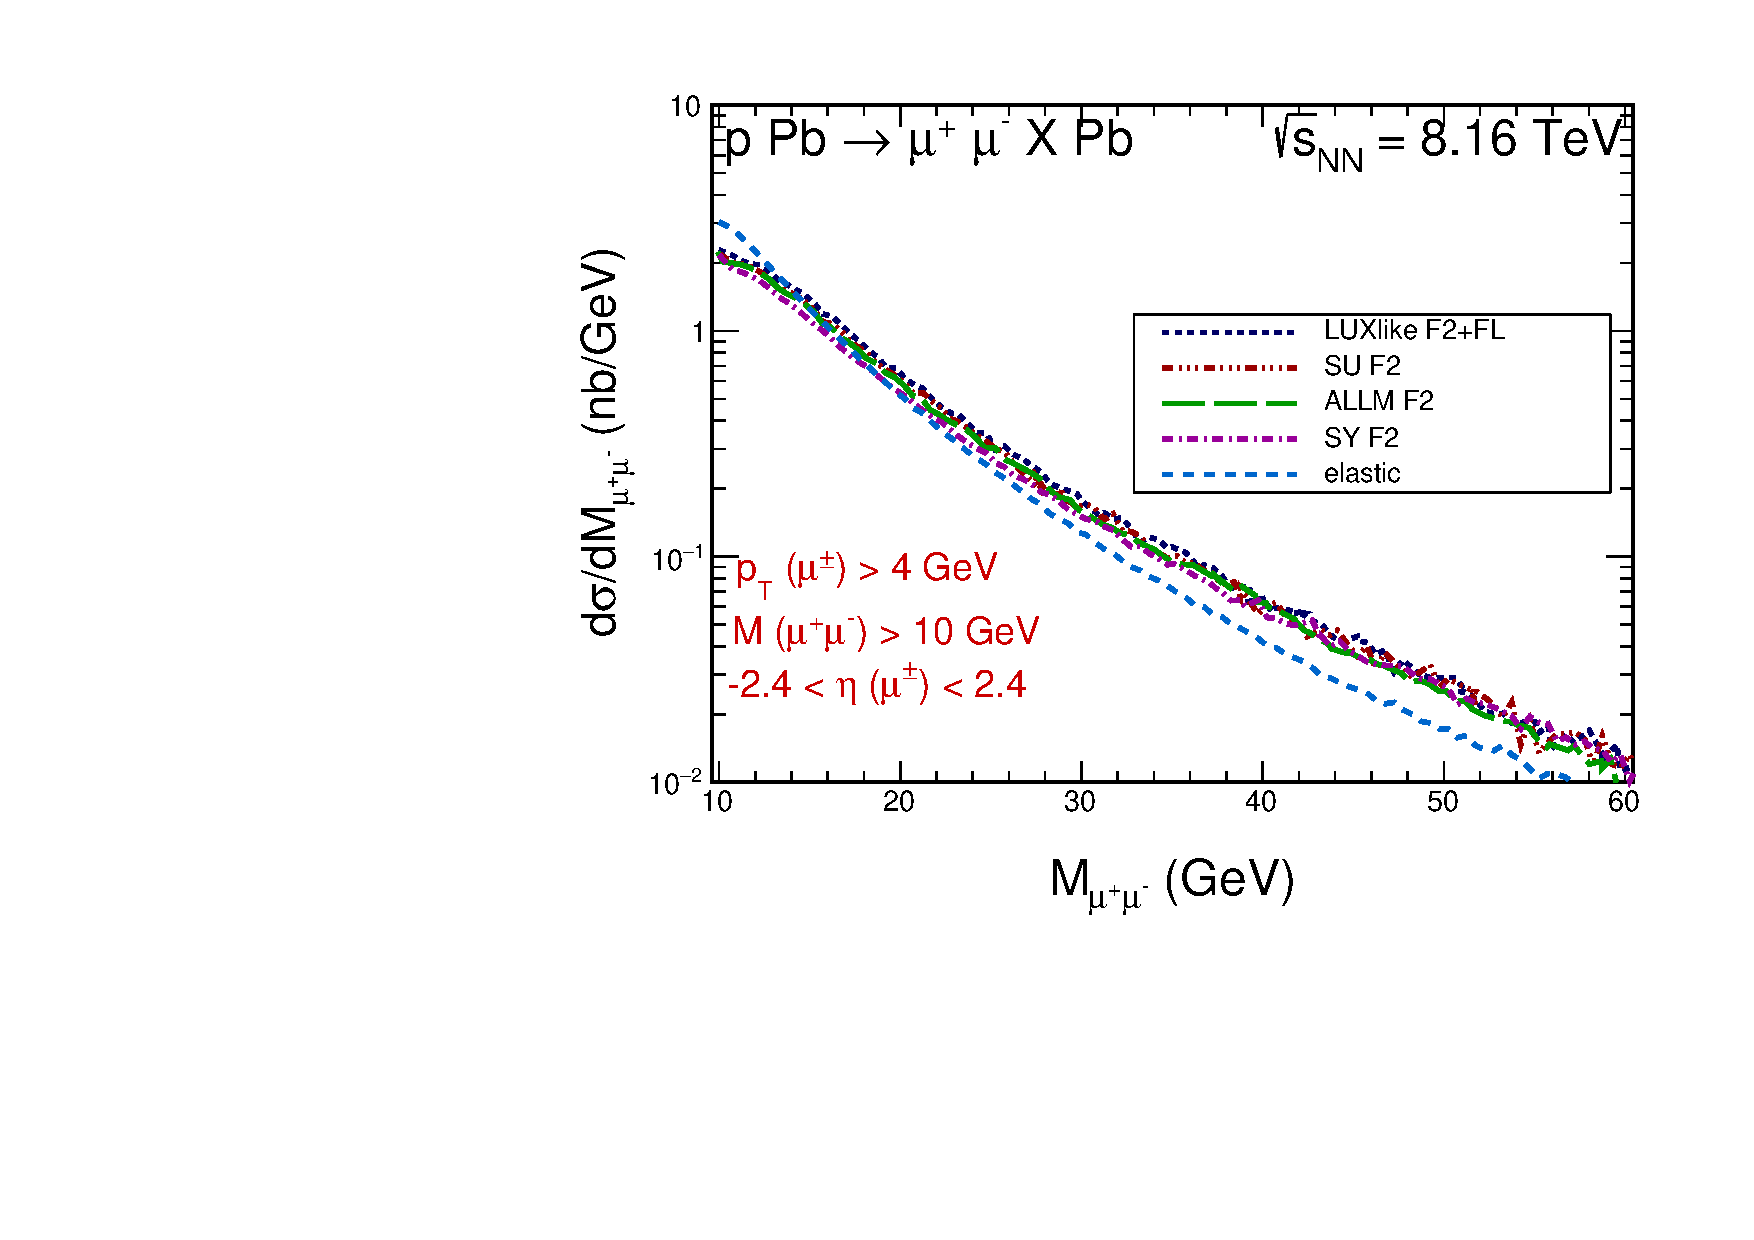
\includegraphics[width=0.49\textwidth]{figures_Marta/Mll-l.pdf}
  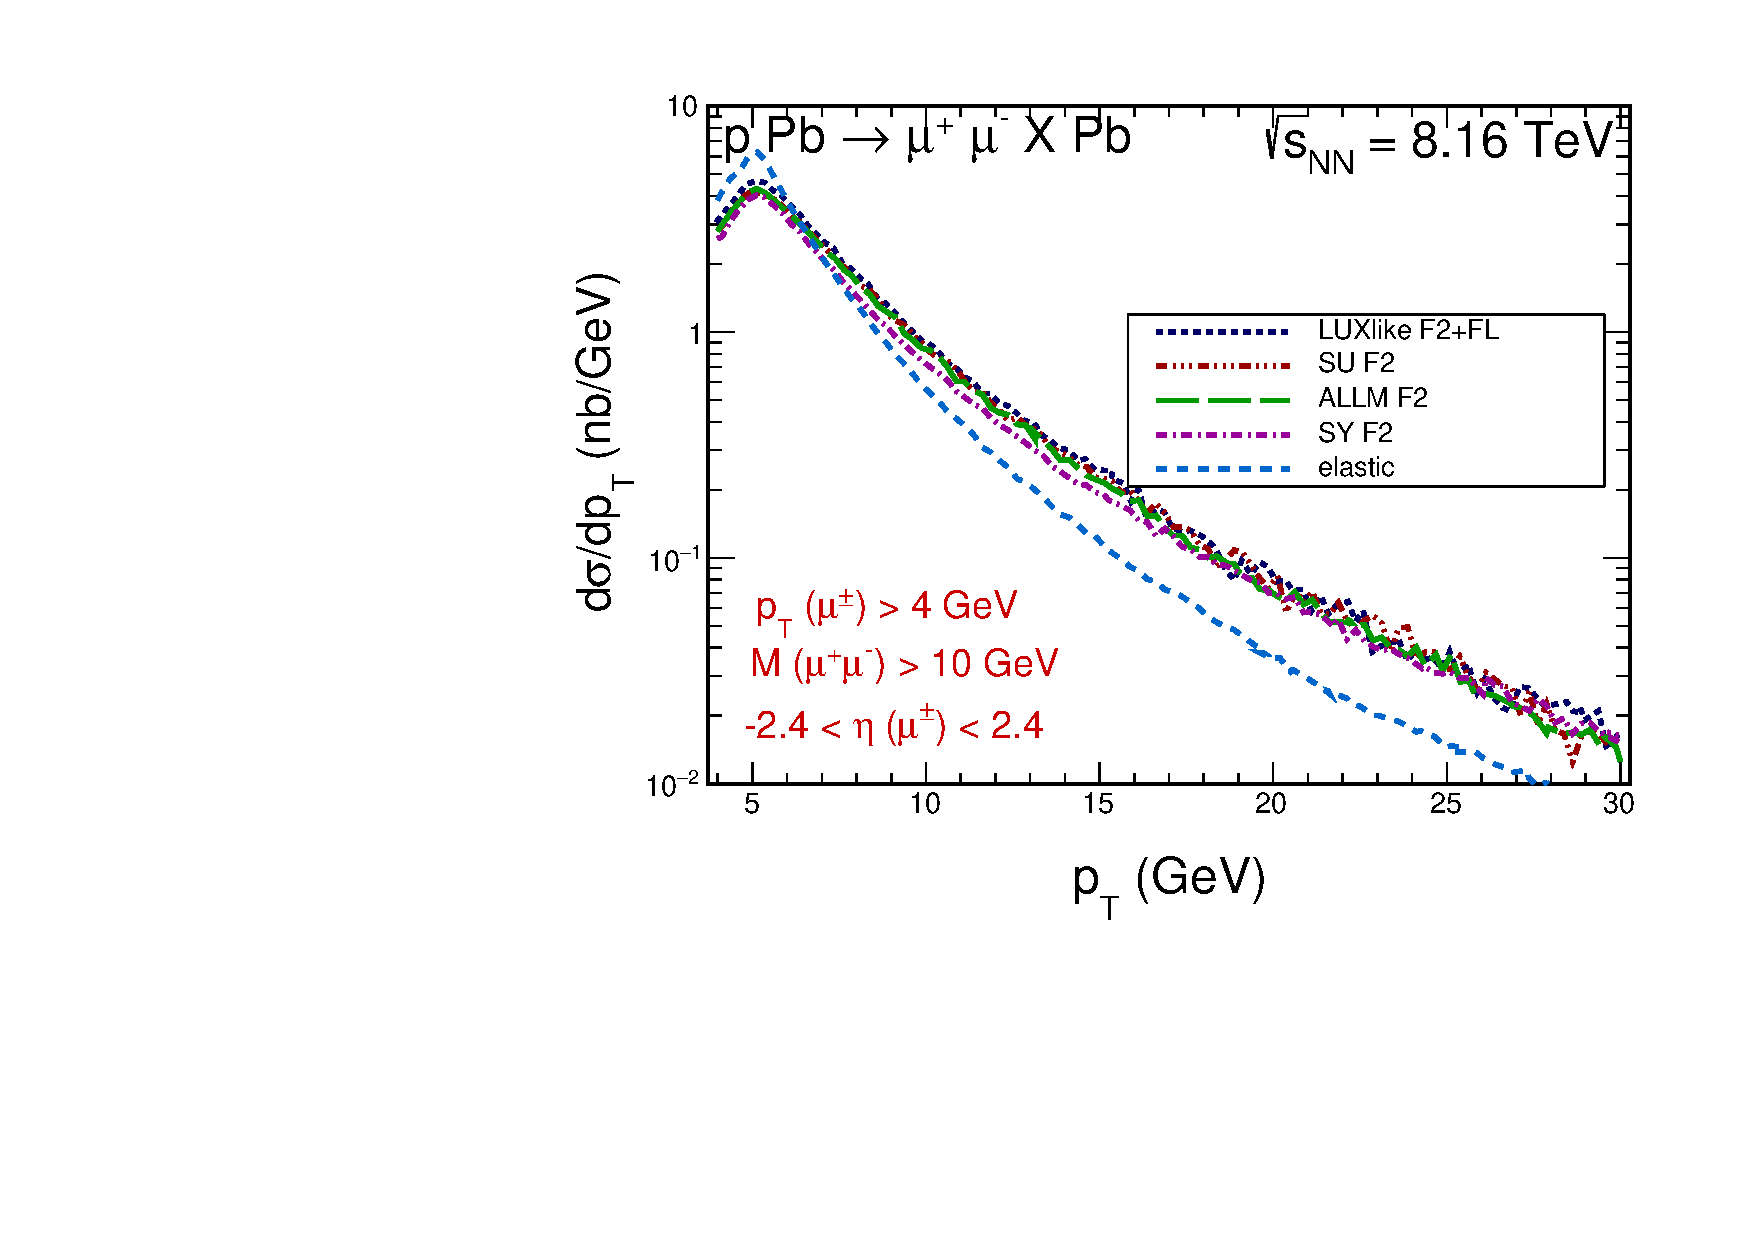
\includegraphics[width=0.49\textwidth]{figures_Marta/pt1-l.pdf}
 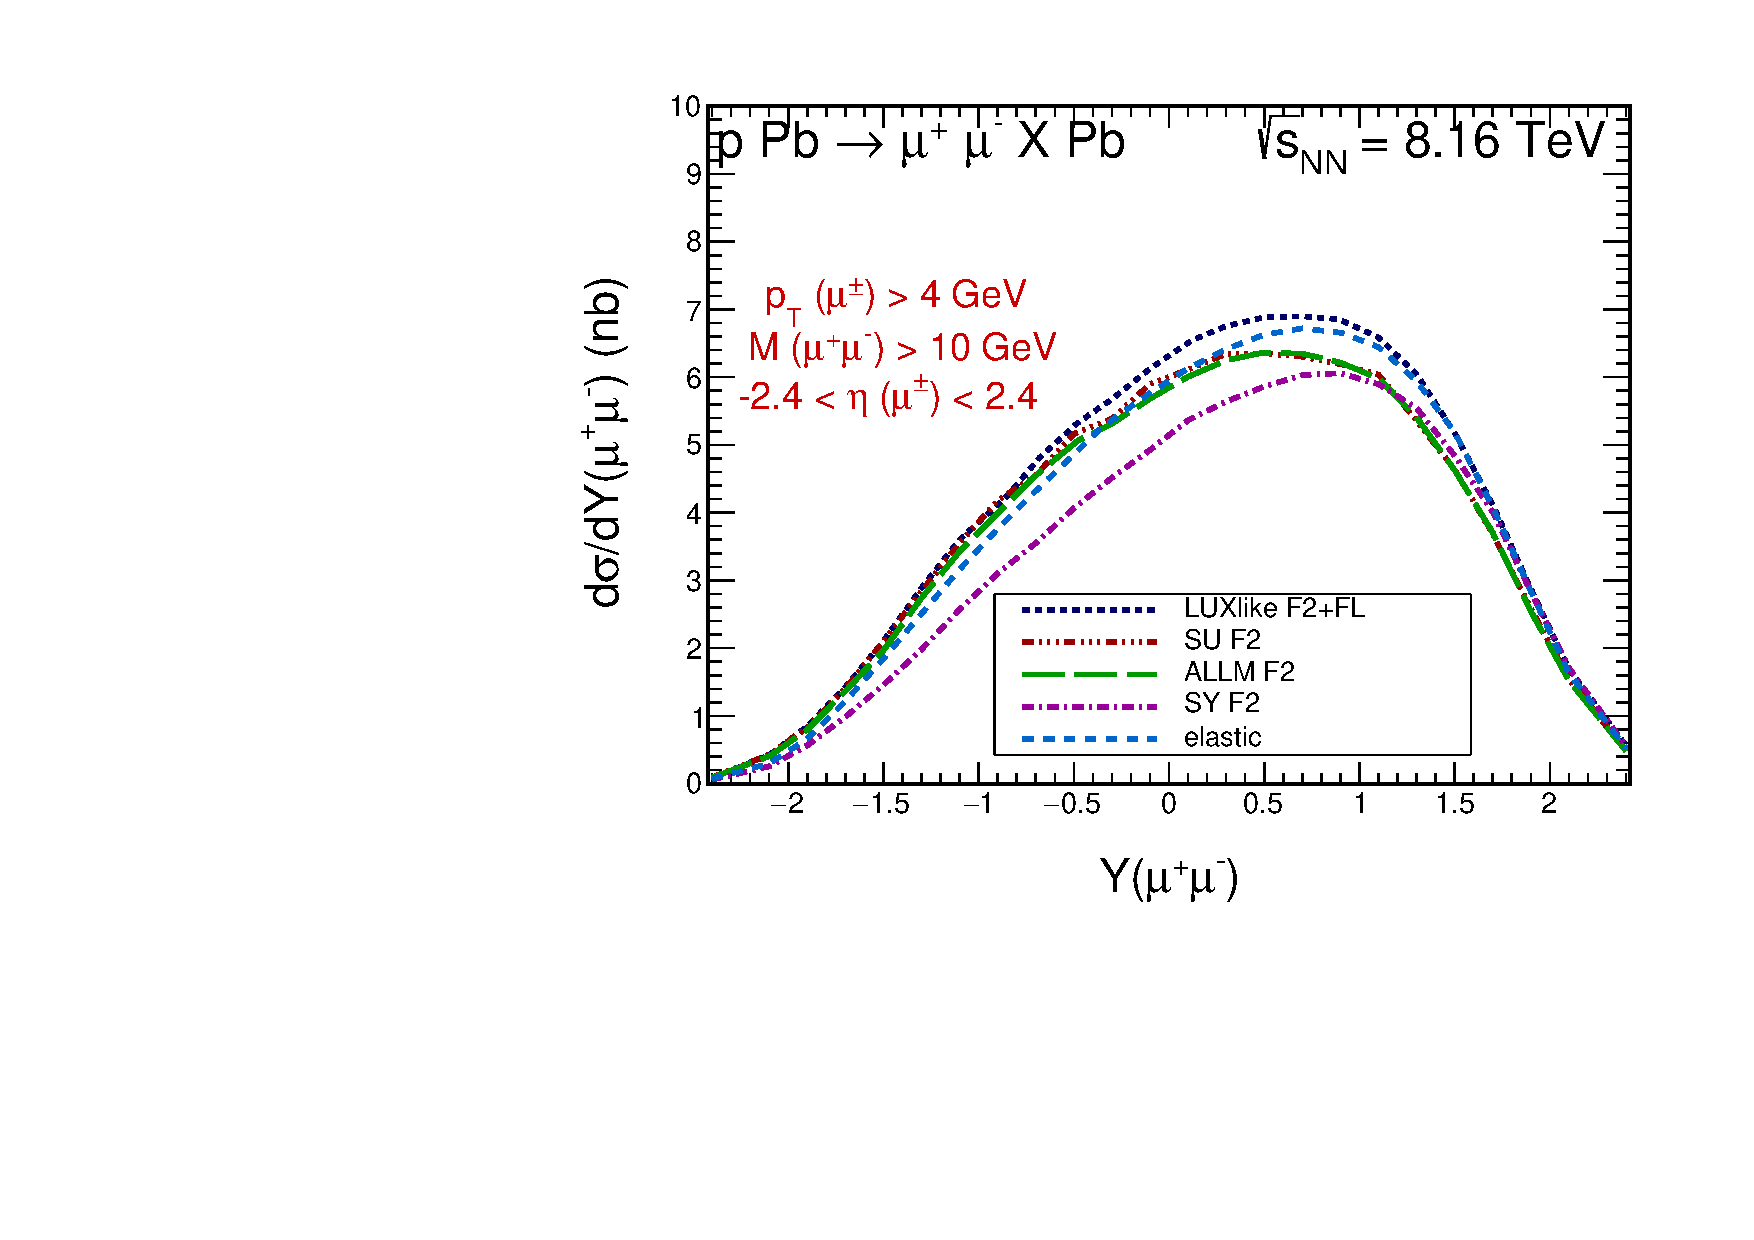
\includegraphics[width=0.49\textwidth]{figures_Marta/Y-l.pdf}
  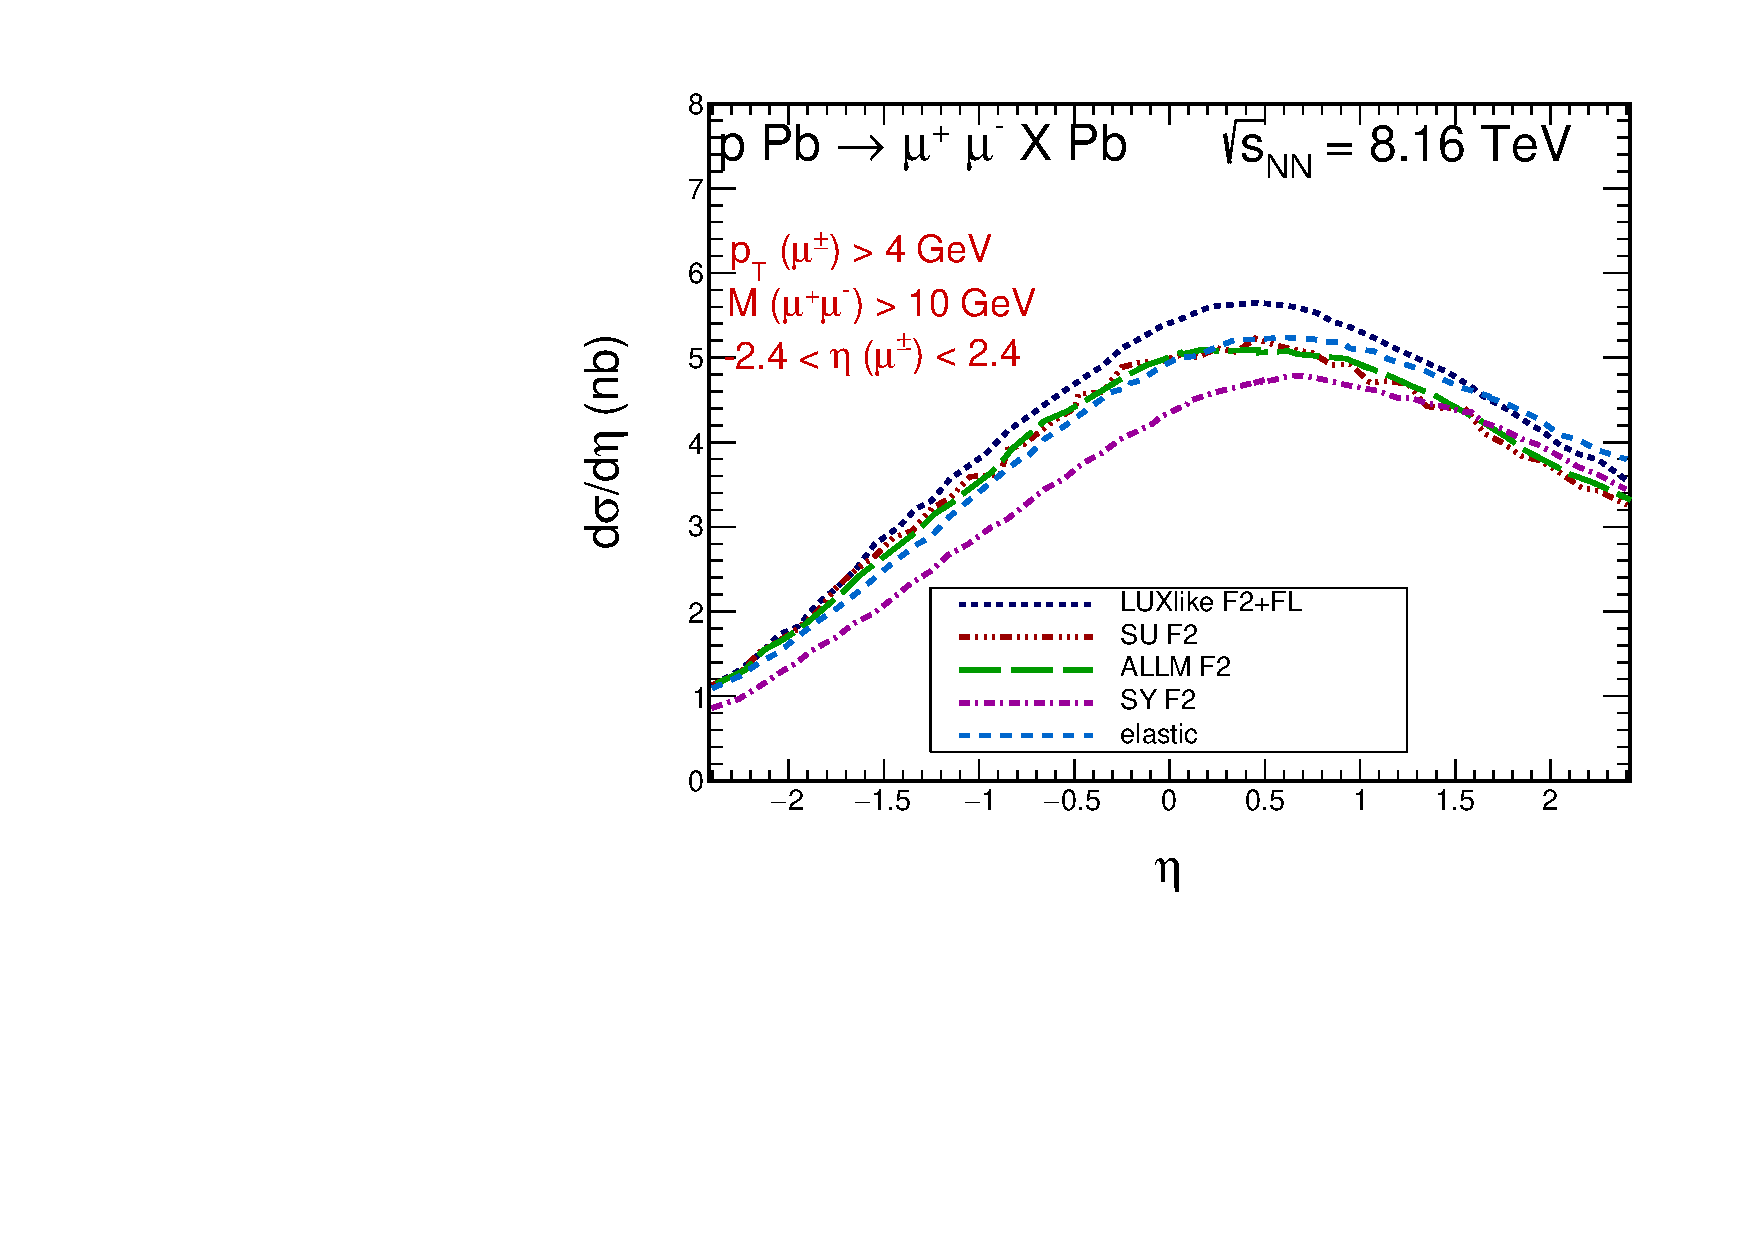
\includegraphics[width=0.49\textwidth]{figures_Marta/y1-l.pdf}
\caption{Differential cross sections in the fiducial region for $p+\textrm{Pb}\rightarrow \textrm{Pb} + \ell^+\ell^- + X$ production at $\sqrt{s_{N N}} = 8.16$~\TeV\ in $k_T$ factorization approach for several proton structure functions.
Four differential distributions are shown: invariant mass of lepton pair (top left), leading lepton transverse momentum (top right),
dilepton rapidity (bottom left) and leading lepton pseudorapidity (bottom right).
For comparison, the elastic contribution ($p+\textrm{Pb}\rightarrow p+ \textrm{Pb} + \ell^+\ell^-$) is also shown.
}
 \label{fig:kt_figures1}
\end{figure}
%------------------------------------------------------------------------------


%-----------------------------------------------------------------------------
\begin{figure}[!h]
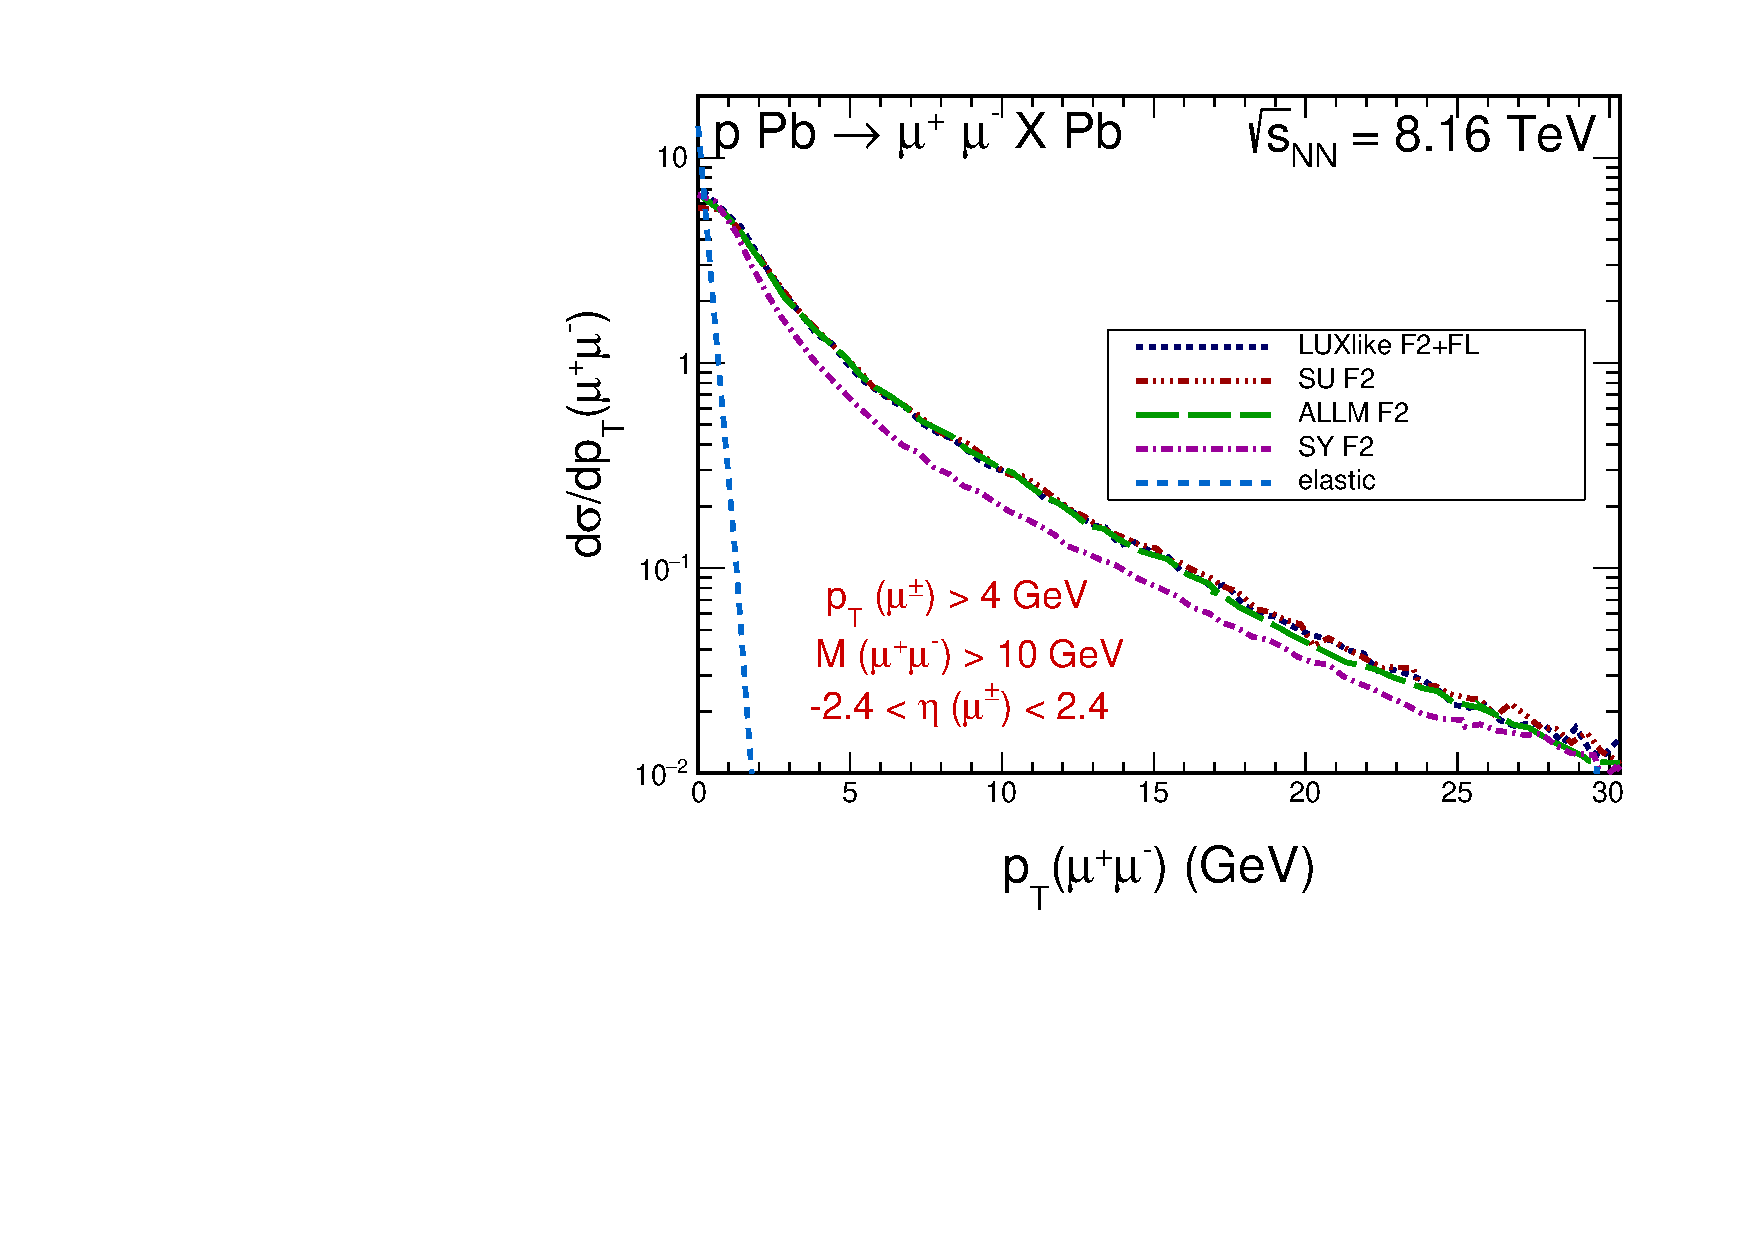
\includegraphics[width=0.49\textwidth]{figures_Marta/pt-sum-l.pdf}
 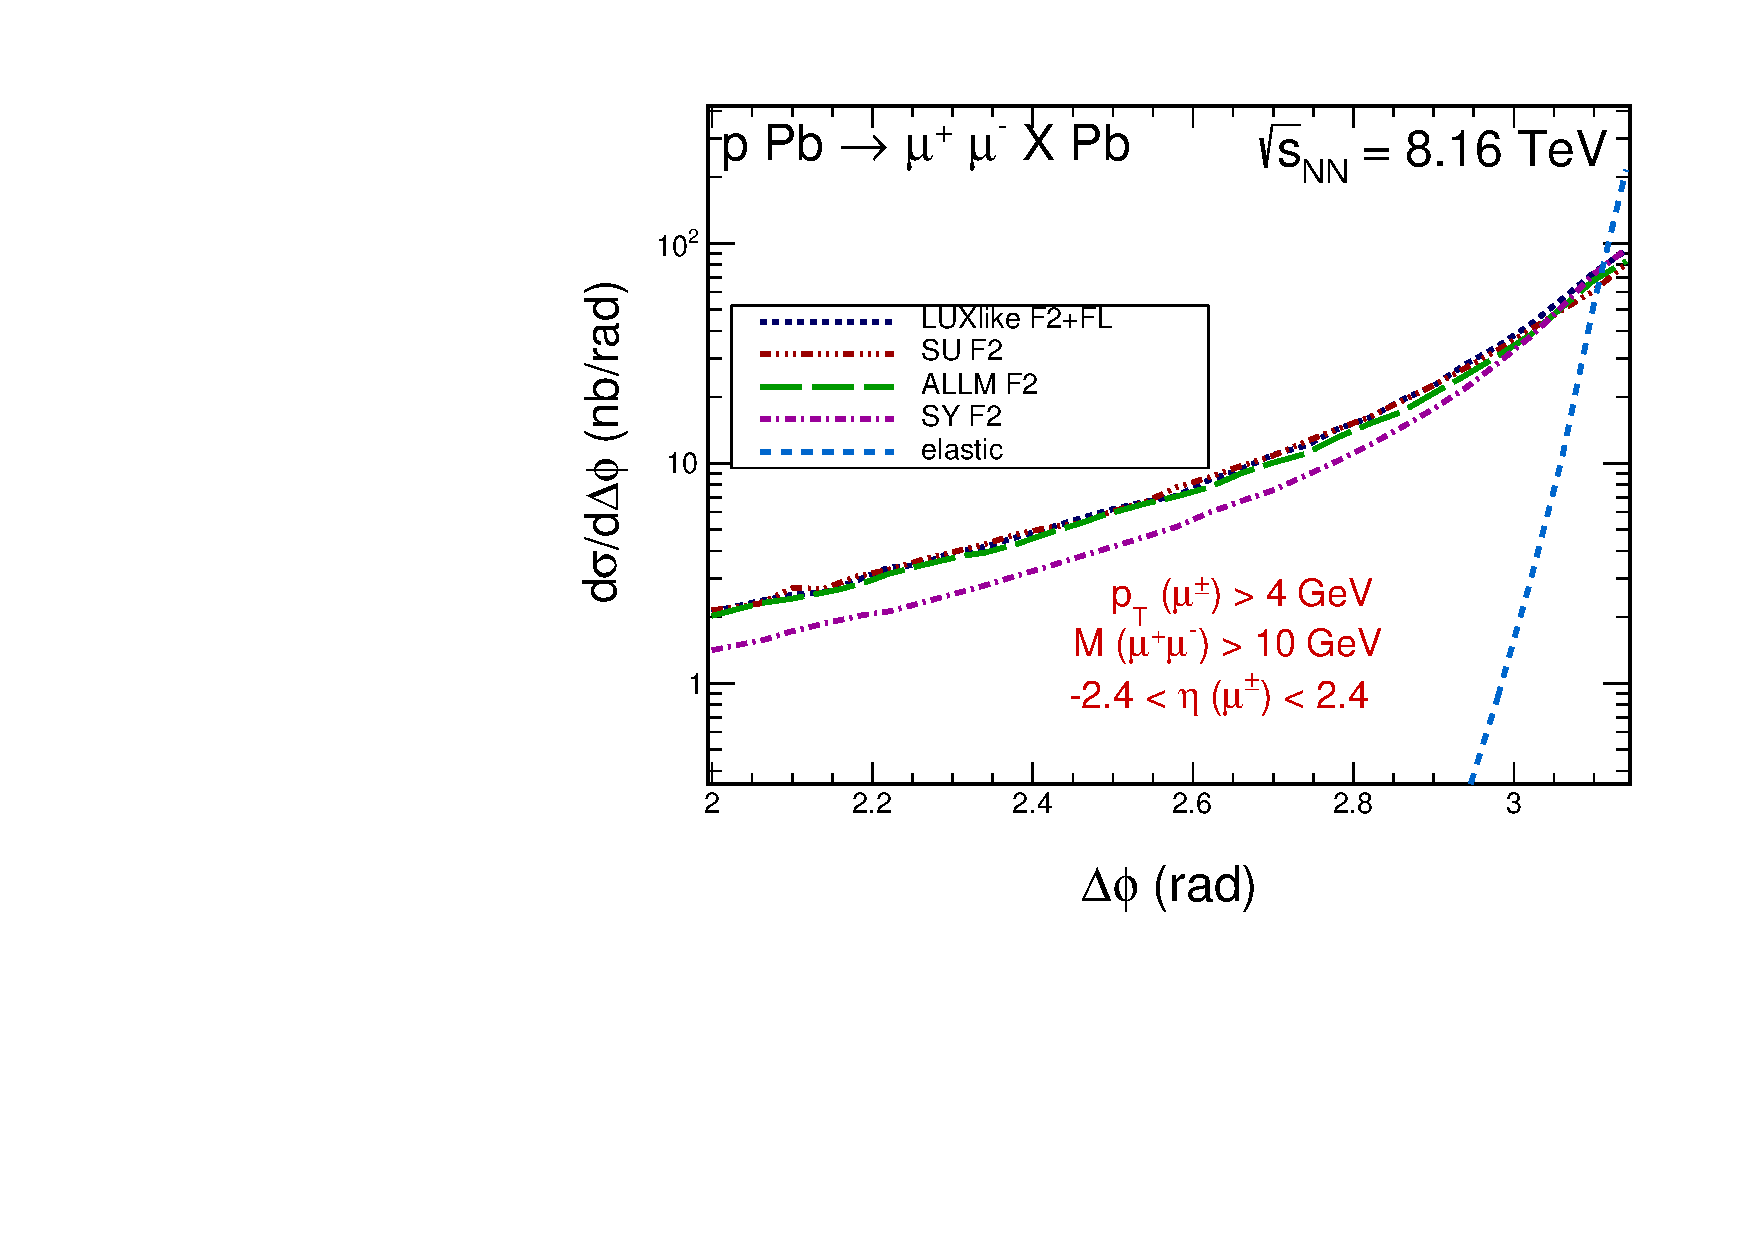
\includegraphics[width=0.49\textwidth]{figures_Marta/phi-l.pdf}
\caption{Differential cross sections in the fiducial region for $p+\textrm{Pb}\rightarrow \textrm{Pb} + \ell^+\ell^- + X$ production at $\sqrt{s_{N N}} = 8.16$~\TeV\ in $k_T$ factorization approach for several proton structure functions.
Two differential distributions are shown: transverse momentum of lepton pair (left) and azimuthal angle difference between the pair (right).
For comparison, the elastic contribution ($p+\textrm{Pb}\rightarrow p+ \textrm{Pb} + \ell^+\ell^-$) is also shown.
}
 \label{fig:kt_figures2}
\end{figure}
%------------------------------------------------------------------------------


%-----------------------------------------------------------------------------
\begin{figure}[!h]

 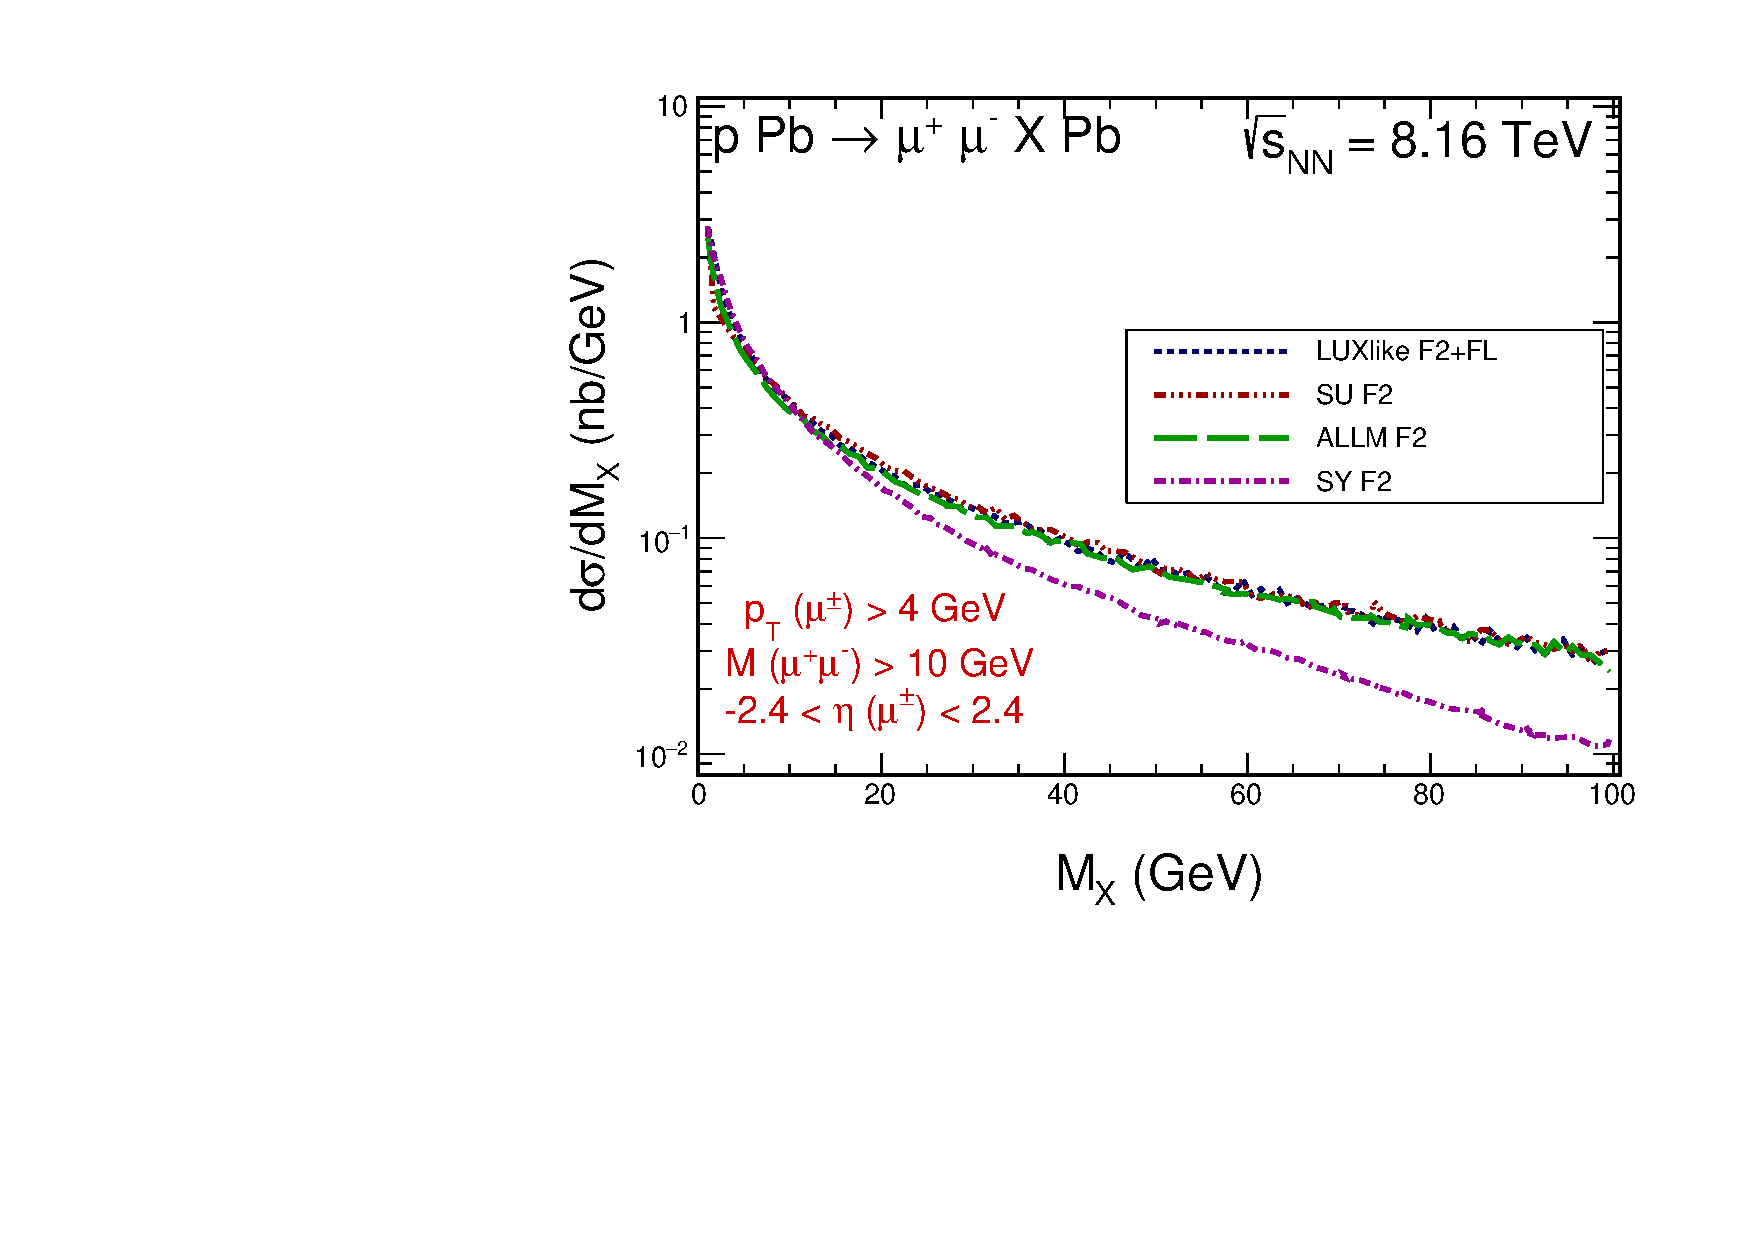
\includegraphics[width=0.49\textwidth]{figures_Marta/MX-l.pdf}
\caption{Differential cross section as a function of the mass of the proton remnants in the fiducial region for $p+\textrm{Pb}\rightarrow \textrm{Pb} + \ell^+\ell^- + X$ production at $\sqrt{s_{N N}} = 8.16$~\TeV\ in $k_T$ factorization approach for several proton structure functions.
For comparison, the elastic contribution ($p+\textrm{Pb}\rightarrow p+ \textrm{Pb} + \ell^+\ell^-$) is also shown.
}
 \label{fig:kt_figures3}
\end{figure}
%------------------------------------------------------------------------------





%
%%-----------------------------------------------------------------------------
%\begin{figure}[!h]
%\begin{minipage}{0.47\textwidth}
% \centerline{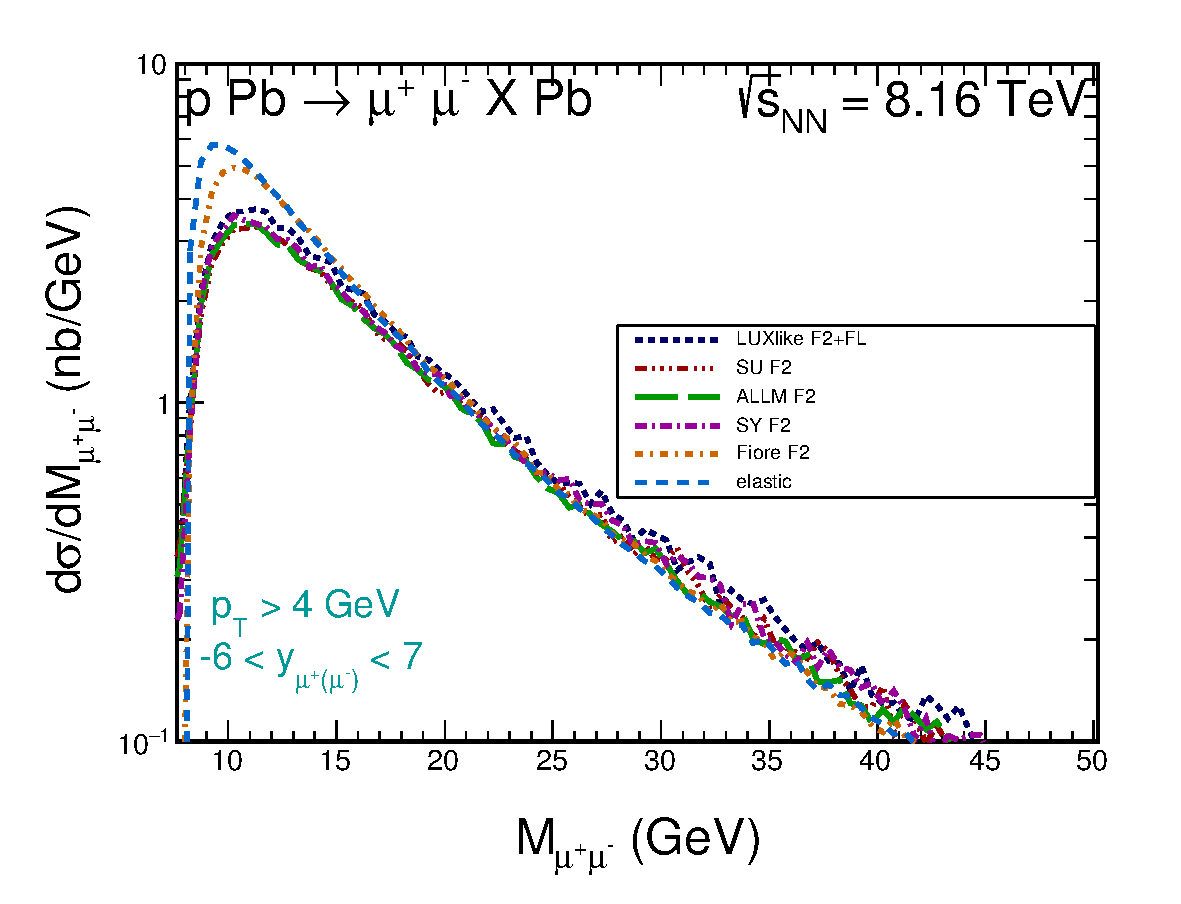
\includegraphics[width=1.0\textwidth]{figures_Marta/Mll.pdf}}
%\end{minipage}
%\begin{minipage}{0.47\textwidth}
% \centerline{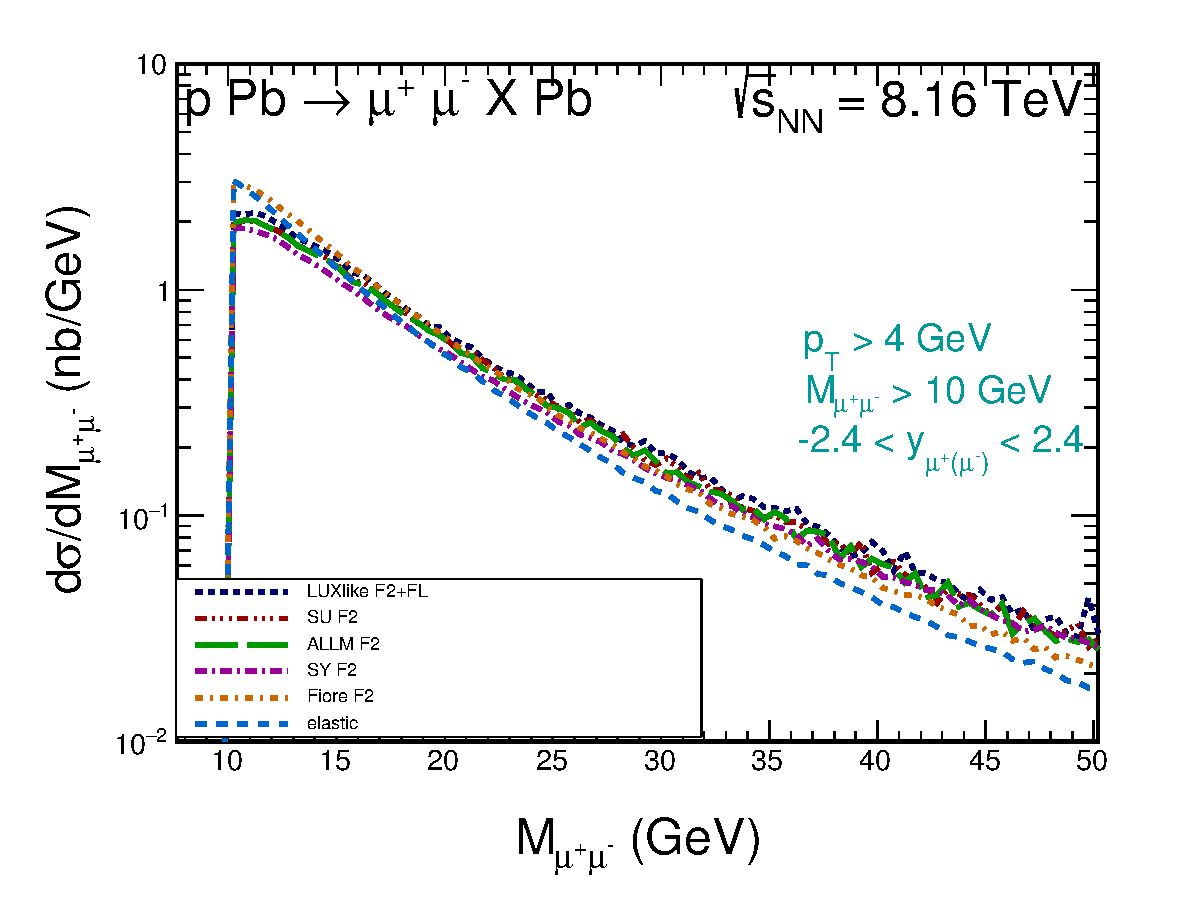
\includegraphics[width=1.0\textwidth]{figures_Marta/Mll-c.pdf}}
%\end{minipage}
%\caption{The elastic - elastic and the inelastic-elastic contribution 
%to dilepton invariant mass distributions 
%for different structure functions. In the left panel we show the results for the whole phase space, while in the right panel only for the fiducial region.
%}
% \label{fig:dsig_dMWW_ineine}
%\end{figure}
%%------------------------------------------------------------------------------
%
%%-----------------------------------------------------------------------------
%\begin{figure}[!htbp]
%\begin{minipage}{0.47\textwidth}
% \centerline{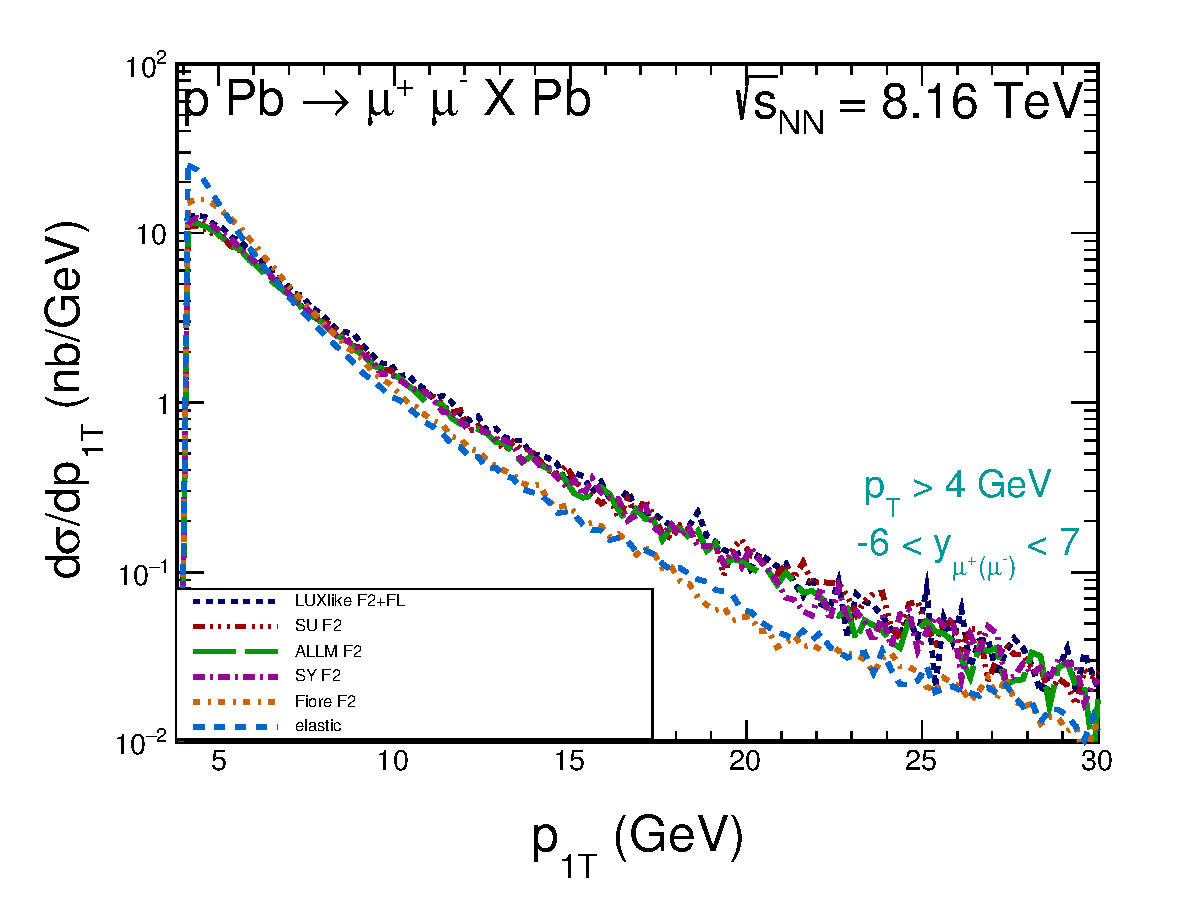
\includegraphics[width=1.0\textwidth]{figures_Marta/pt1.pdf}}
%\end{minipage}
%\begin{minipage}{0.47\textwidth}
% \centerline{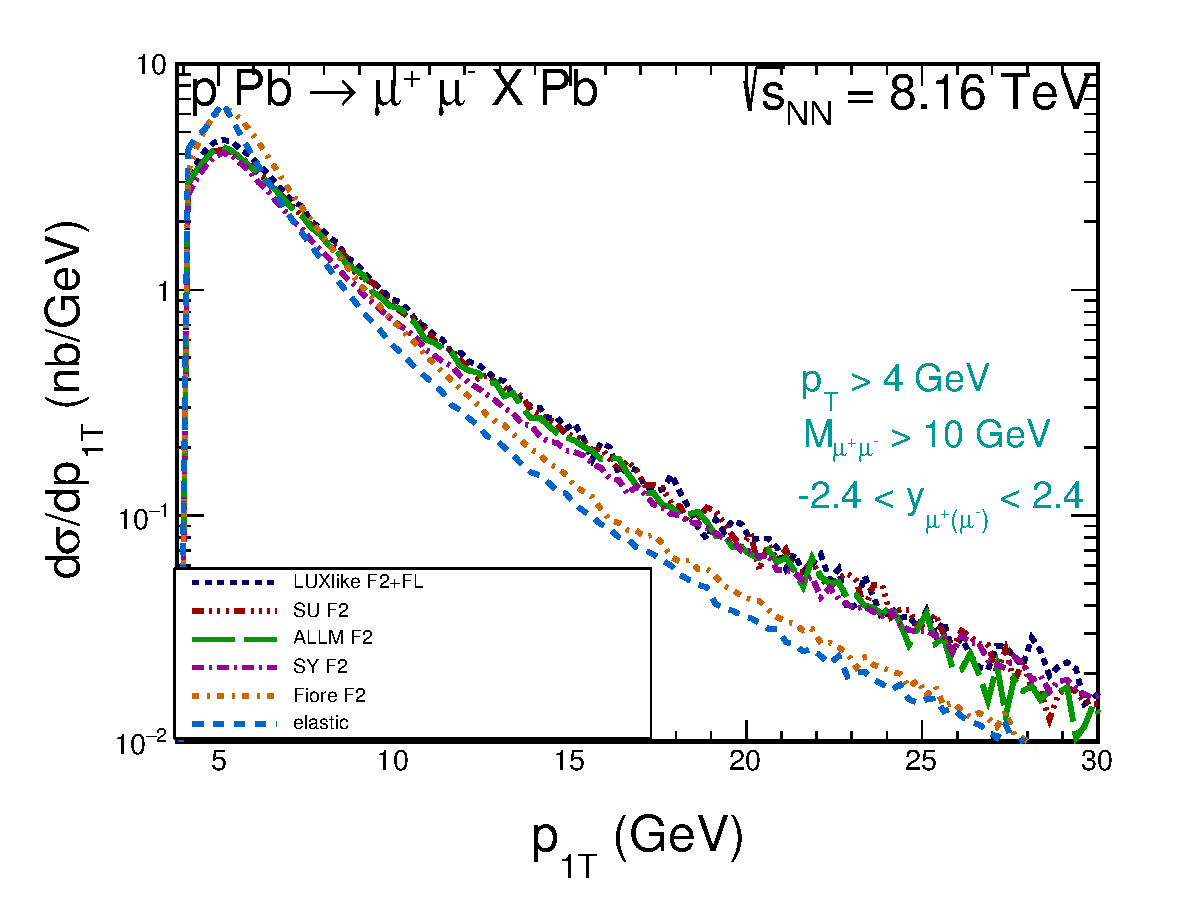
\includegraphics[width=1.0\textwidth]{figures_Marta/pt1-c.pdf}}
%\end{minipage}
%\caption{
%Transverse momentum distribution of $\mu^+$ or $\mu^-$ 
%for elastic - elastic and inelastic - elastic different structure functions: LUX-like, ALLM97, Fiore at all., SU and SY (in the left panel we show the results for the whole phase space, while in the right panel only for the fiducial region).
%}
% \label{fig:dsig_dMWW_ineine}
%\end{figure}
%%------------------------------------------------------------------------------
%
%
%%-----------------------------------------------------------------------------
%\begin{figure}[!htbp]
%\begin{minipage}{0.47\textwidth}
% \centerline{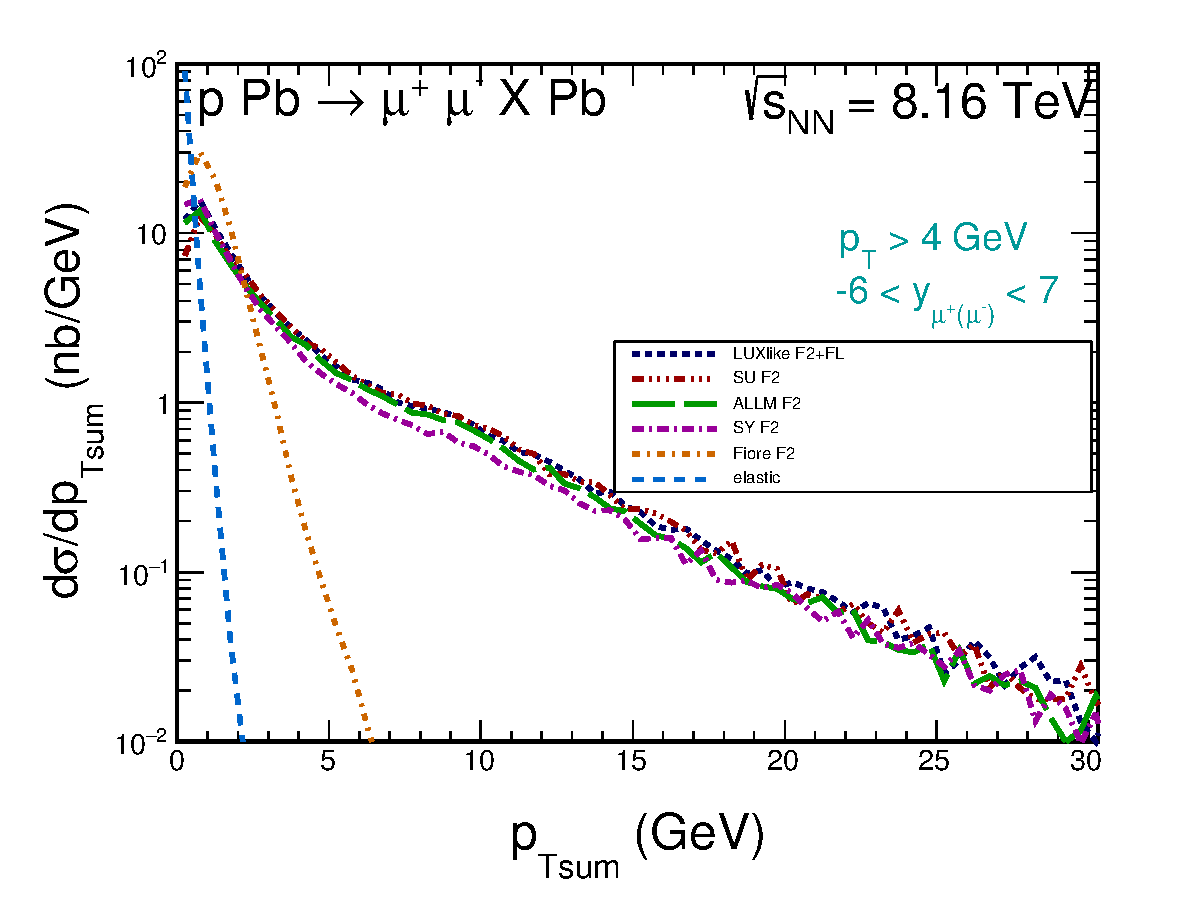
\includegraphics[width=1.0\textwidth]{figures_Marta/ptsum.pdf}}
%\end{minipage}
%\begin{minipage}{0.47\textwidth}
% \centerline{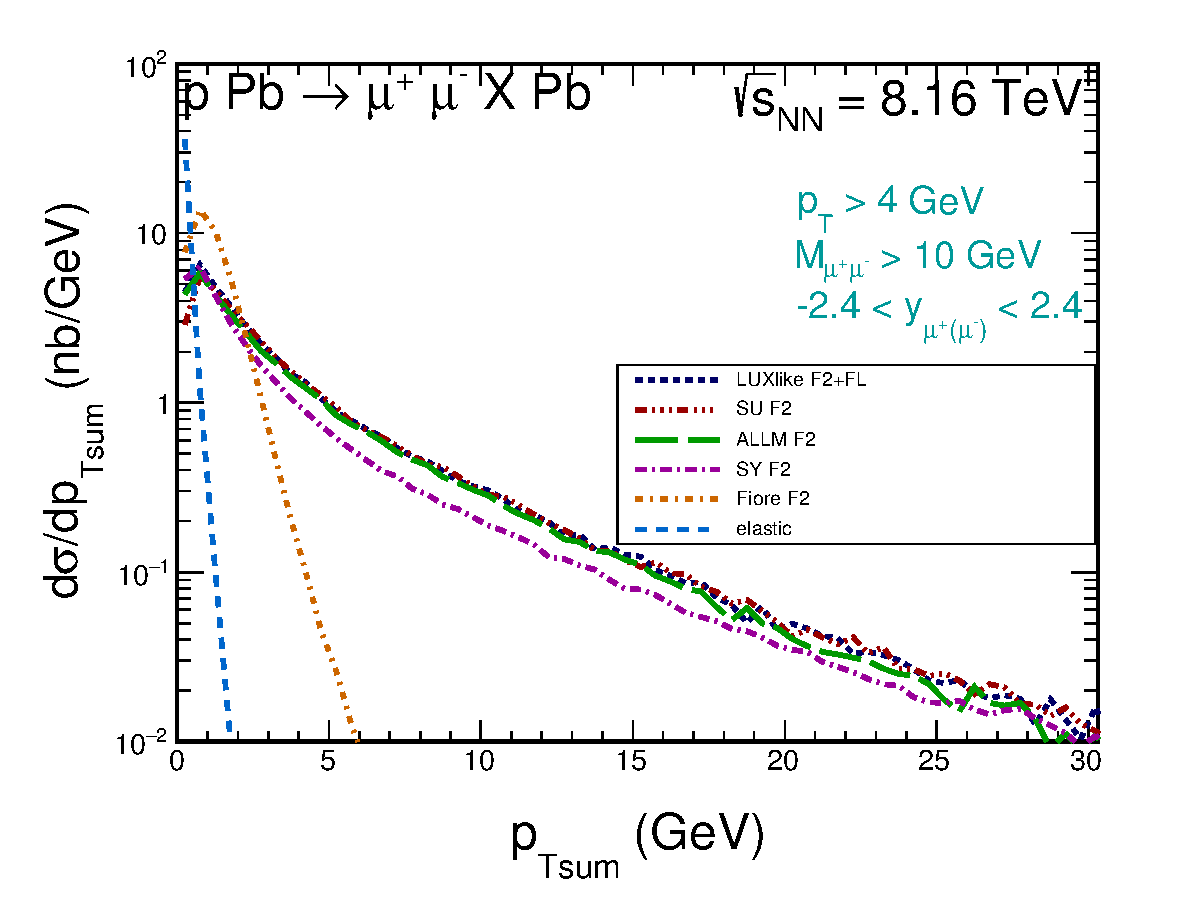
\includegraphics[width=1.0\textwidth]{figures_Marta/ptsum-c.pdf}}
%\end{minipage}
%\caption{
%Distribution in transverse momentum of the $\mu^+ \mu^-$ pairs for elastic - elastic and 
%inelastic-elastic
%contributions
%for different structure functions: LUX-like, ALLM97, Fiore at all., SU and SY. (in the left panel we show the results for the whole phase space, while in the right panel only for the fiducial region).
%}
% \label{fig:dsig_dMWW_ineine}
%\end{figure}
%%------------------------------------------------------------------------------
%
%
%%-----------------------------------------------------------------------------
%\begin{figure}[!htbp]
%\begin{minipage}{0.47\textwidth}
% \centerline{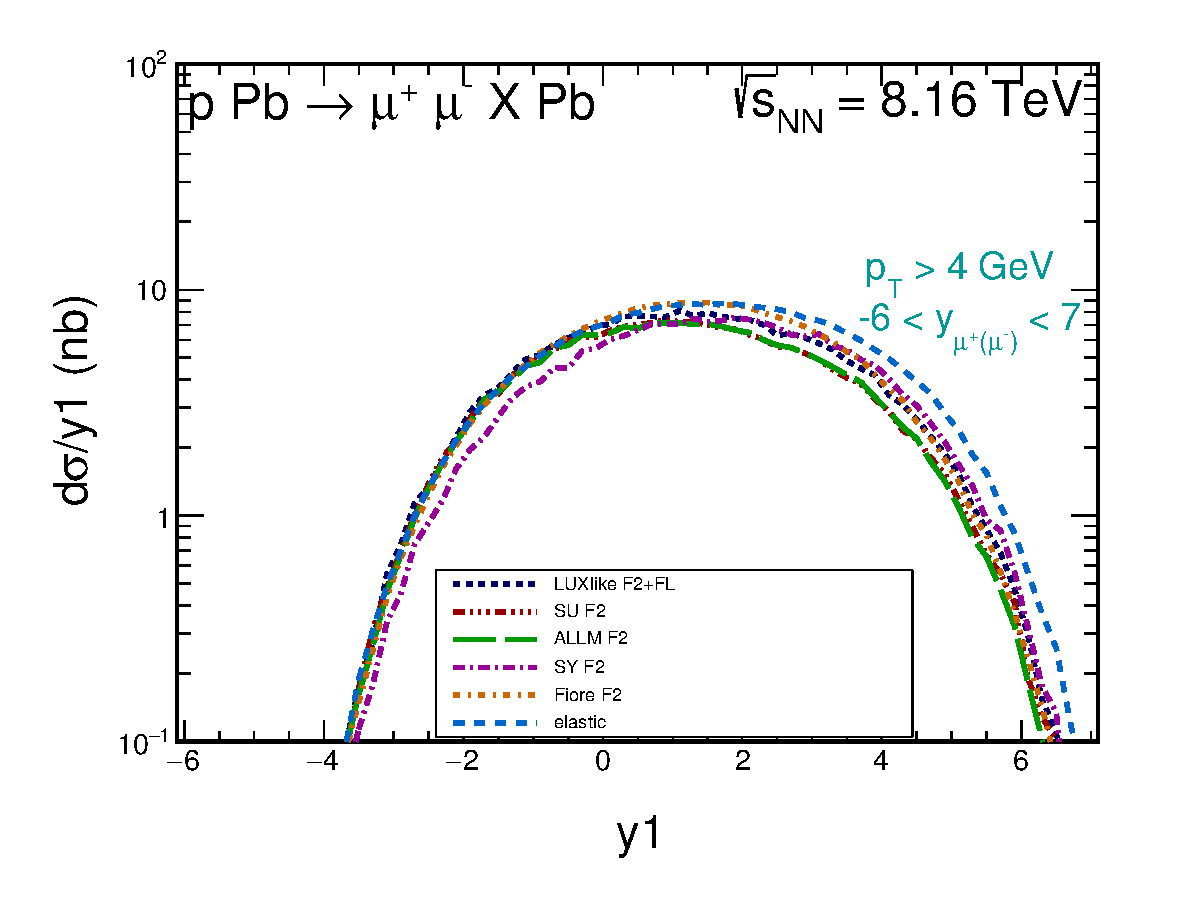
\includegraphics[width=1.0\textwidth]{figures_Marta/y1.pdf}}
%\end{minipage}
%\begin{minipage}{0.47\textwidth}
% \centerline{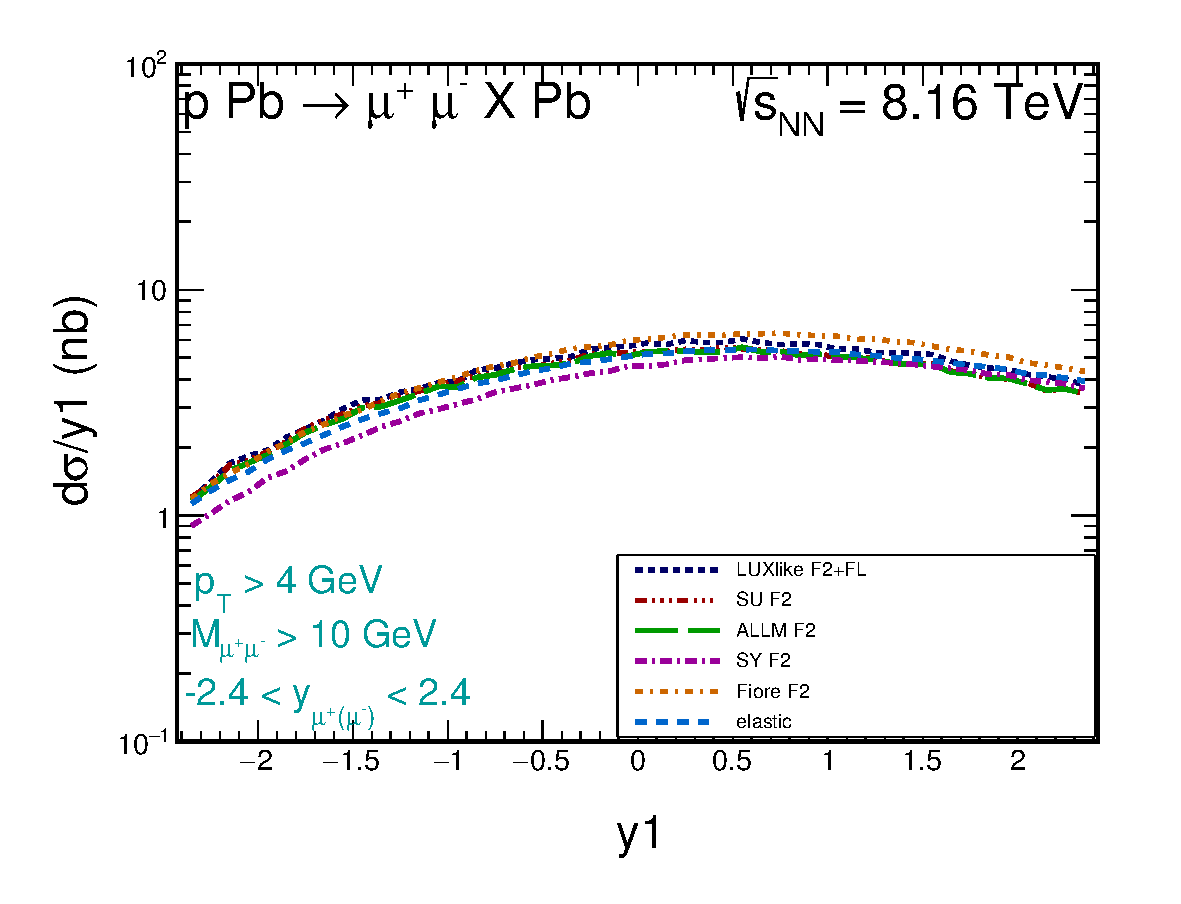
\includegraphics[width=1.0\textwidth]{figures_Marta/y1-c.pdf}}
%\end{minipage}
%
%\caption{
%Rapidity distribution of $\mu^+$ or $\mu^-$ leptons
%for elastic - elastic and inelastic-elastic contributions for different structure functions: LUX-like, ALLM97, Fiore at all., SU and SY. (in the left panel we show the results for the whole phase space, while in the right panel only for the fiducial region).
%}
% \label{fig:dsig_dMWW_ineine}
%\end{figure}
%%------------------------------------------------------------------------------
%
%
%
%%------------------------------------------------------------------------------
%
%%-----------------------------------------------------------------------------
%\begin{figure}[!htbp]
%\begin{minipage}{0.47\textwidth}
% \centerline{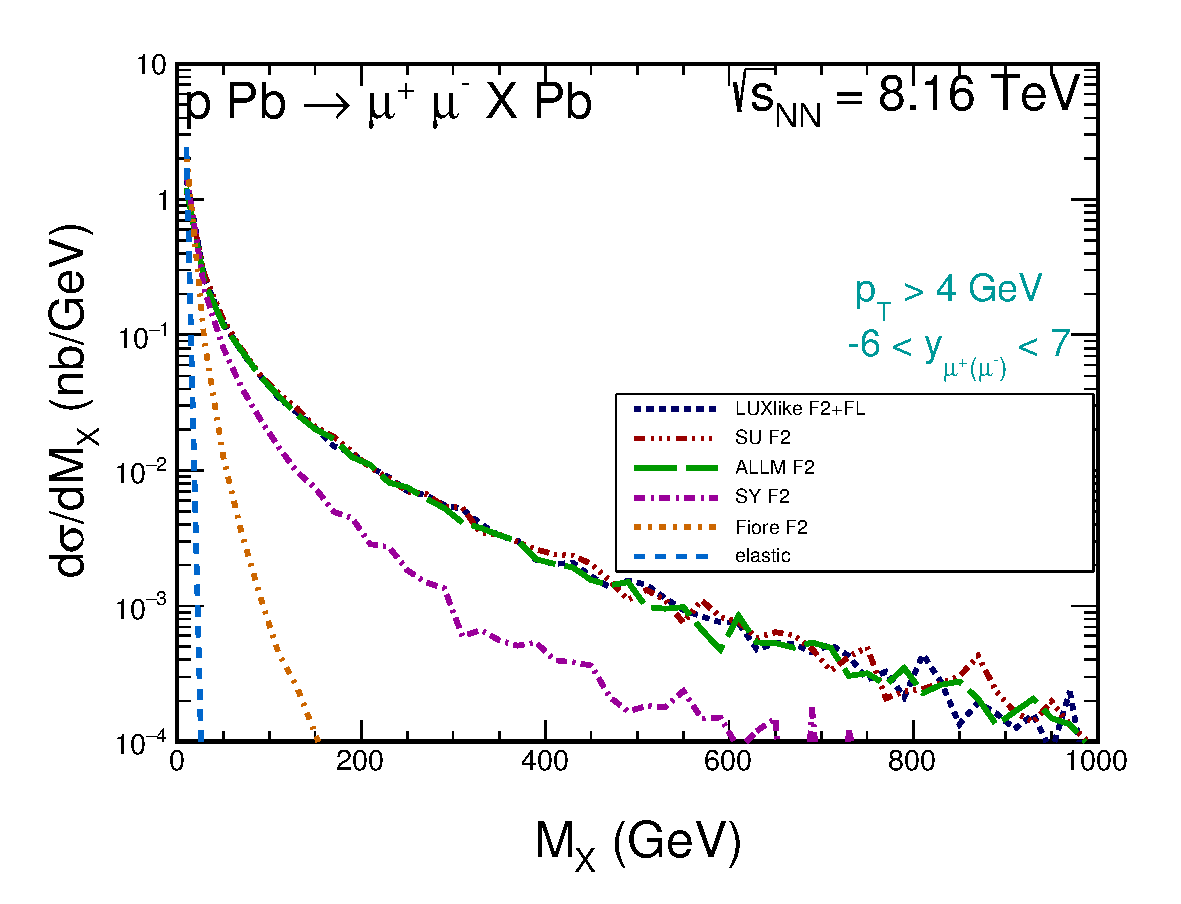
\includegraphics[width=1.0\textwidth]{figures_Marta/MX.pdf}}
%\end{minipage}
%%\hspace{0.5cm}
%\begin{minipage}{0.47\textwidth}
% \centerline{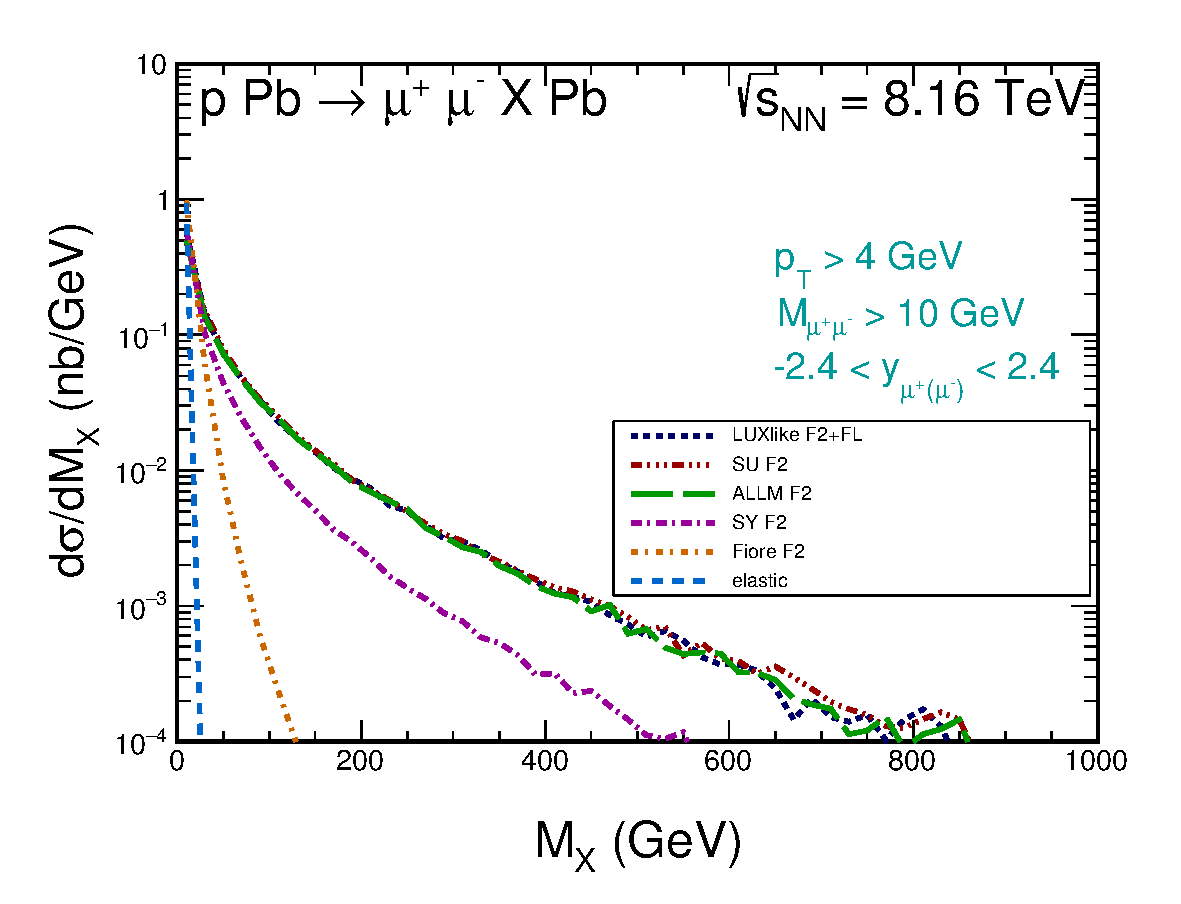
\includegraphics[width=1.0\textwidth]{figures_Marta/MX-c.pdf}}
%\end{minipage}
%\caption{
%Missing mass distributions for eleastic-elastic photon-photon contributions and elastic-inelastic photon-photon contributions for different structure functions: LUX-like, ALLM97, Fiore at all., SU and SY. (in the left panel we show the results for the whole phase space, while in the right panel only for the fiducial region).
%}
%\label{fig:dsig_dy}
%\end{figure}
%%---------------------------------------------------------------
%
%
%
%
%%-----------------------------------------------------------------------------
%\begin{figure}[!htbp]
%\begin{minipage}{0.47\textwidth}
% \centerline{\includegraphics[width=1.0\textwidth]{figures_Marta/ydiff.pdf}}
%\end{minipage}
%%\hspace{0.5cm}
%\begin{minipage}{0.47\textwidth}
% \centerline{\includegraphics[width=1.0\textwidth]{figures_Marta/ydiff-c.pdf}}
%\end{minipage}
%\caption{
%Distribution in rapidity distance between $\mu^+\mu^-$ leptons.
%The calculation for the $\gamma-\gamma$ contribution
%was performed for different structure functions. 
%The left panel shows results  without cuts while the right panel 
%shows results with ATLAS cuts.
%}
%\label{fig:dsig_dy}
%\end{figure}
%%---------------------------------------------------------------
%
%%-----------------------------------------------------------------------------
%\begin{figure}[!htbp]
%\begin{minipage}{0.47\textwidth}
% \centerline{\includegraphics[width=1.0\textwidth]{figures_Marta/phi.pdf}}
%\end{minipage}
%%\hspace{0.5cm}
%\begin{minipage}{0.47\textwidth}
% \centerline{\includegraphics[width=1.0\textwidth]{figures_Marta/phi-c.pdf}}
%\end{minipage}
%\caption{
%Distributions for azimuthal angle between $\mu^+\mu^-$ leptons. (in the left panel we show the results for the whole phase space, while in the right panel only for the fiducial region).
%}
%\label{fig:dsig_dy}
%\end{figure}
%%---------------------------------------------------------------





\clearpage
%%%%%%%%%%%%%%%%%%%%%%%%%%%%%%%%%%
\section{Discussion}
%%%%%%%%%%%%%%%%%%%%%%%%%%%%%%%%%%

We take the opportunity to calculate expected number of events for realistic assumption on total integrated luminosity.
Based on the previous $p\textrm{Pb}$ runs at the LHC, we assume  $\int Ldt= 200~\textrm{nb}^{-1}$.
We also assume possible experimental efficiencies, manily due to trigger and recontruction of leptons, which we embed in a single correction factor $C=0.7$.

Table~\ref{fig:numbers} shows the expected number of events for $p+\textrm{Pb}\rightarrow \textrm{Pb} + \ell^+\ell^- + X$ production at $\sqrt{s_{N N}} = 8.16$~\TeV\ and configuration described above. 
Approximately 2500 elastic dilepton events are expected. 
Depending on the calculations, 3900 (collinear with LUXqed17 PDF) or 2400 ($k_T$-factorization with LUX-like $F_2+F_L$) inelastic events (reconstructed) are predicted. The difference between collinear and $k_T$-factorization can be therefore constrained with large significance, using existing datasets collected by ATLAS and CMS.

\begin{table}[t]
\begin{center}
\begin{tabular}{|l|c|c|}
\hline
Contribution & Expected events ($C=1$) & Expected events ($C=0.7$) \\
\hline
%$\gamma^{p}_{\rm{el}}$ [$b_{min}=0.7fm$] & 45.5(2) nb & 17.3(1) nb\\
%\hline
$\gamma^{p}_{\rm{el}}$  & 3600 & 2500\\ % [Electric]
\hline
$\gamma^{p}_{\rm{inel}}$ [LUXqed17 collinear] & 5600 & 3900 \\
\hline
$\gamma^{p}_{\rm{inel}}$ [LUX-like $F_2+F_L$] & 3400 & 2400 \\
\hline
\end{tabular}
\end{center}
\caption{Expected number of events for $p+\textrm{Pb}\rightarrow \textrm{Pb} + \ell^+\ell^- + X$ production at $\sqrt{s_{N N}} = 8.16$~\TeV\ assuming $\int Ldt= 200~\textrm{nb}^{-1}$. 
Shown are several contributions: purely elastic, inelastic with collinear LUXqed17 PDF and inelastic with $k_T$-factorization and LUX-like $F_2+F_L$ proton structure function parameterization.
An effect of possible experimental efficiencies is shown in last column.}
\label{fig:numbers}
\end{table}
%%%%%%%%%%%%%%%%%%%%%%%%%%%%%%%%%%
\section{Summary}
%%%%%%%%%%%%%%%%%%%%%%%%%%%%%%%%%%

In summary, we propose a method that would unambiguously allow to test and constrain the photon parton distribution at LHC energies.

%%%%%%%%%%%%%%%%%%%%%%%%%%%%%%%%%%



\section*{References}
%\clearpage
\bibliographystyle{atlasnote}
\bibliography{main}


\end{document}

